
Let $\legendrian\subset J^1\sphere^1$ be a Legendrian knot or link which is a closure of a positive braid and bounds a Legendrian surface~$\Legendrian(\ngraph)$ in $J^1\disk^2$ for some free $N$-graph $\ngraph$.
We fix a set $\nbasis$ of good cycles in the sense of Definition~\ref{def:good cycle}.
Then, by Theorem~\ref{thm:N-graph to seed}, we obtain a $Y$-seed $\Psi(\ngraph,\nbasis)$ which is a pair of a coefficient tuple~$\bfy(\Legendrian(\ngraph),\nbasis)$ 
and a quiver $\quiver(\Legendrian(\ngraph),\nbasis)$. 

We say that the pair $(\ngraph,\nbasis)$ is \emph{of finite type} or \emph{of
infinite type} if so is the cluster algebra defined by
$\quiver(\Legendrian(\ngraph),\nbasis)$.
Similarly, it is said to be \emph{of type $\dynX$} for some Dynkin diagram $\dynX$ if so is the associated cluster algebra.

In particular, it is said to be \emph{of type~$\dynADE$} or \emph{of affine type} if the quiver is of type $\dynADE$ or of affine type. See Definition~\ref{def_quiver_of_type_X}.


\subsection{\texorpdfstring{$N$-graphs}{N-graphs} of finite or affine types}

\subsubsection{Linear \texorpdfstring{$N$-graphs}{N-graphs}}\label{sec:linear}
For $n\ge 1$, let us define positive $2$-braids
\begin{align*}
\beta_0(\dynA_n)&\colonequals \sigma_1^{n+1},&
\beta(\dynA_n) &\colonequals \sigma_1^{n+3} = \Delta_2 \beta_0(n) \Delta_2,
\end{align*}
where $\Delta_N$ is the half-twist braid of $N$-strands.
Then we define $\legendrian(\dynA_n)$ be the rainbow closure of~$\beta_0(\dynA_n)$.
\begin{align*}
&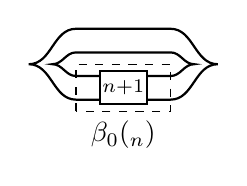
\begin{tikzpicture}[baseline=-.5ex,scale=0.6]
\draw[thick] (-0.5,-0.25) -- (-1,-0.25) to[out=180,in=0] (-1.5,0) to[out=0,in=180] (-1,0.25) -- (1,0.25) to[out=0,in=180] (1.5,0) to[out=180,in=0] (1,-0.25) -- (0.5, -0.25);
\draw[thick] (-0.5,-0.75) -- (-1,-0.75) to[out=180,in=0] (-2,0) to[out=0,in=180] (-1,0.75) -- (1,0.75) to[out=0,in=180] (2,0) to[out=180,in=0] (1,-0.75) -- (0.5,-0.75);
\draw[thick] (-0.5,-0.85) rectangle (0.5,-0.15);
\draw (0,-0.5) node {$\scriptstyle n+1$};
\draw[dashed] (-1,-1) rectangle (1,0) (0,-1) node[below] {$\beta_0(\dynA_n)$};
\end{tikzpicture}&
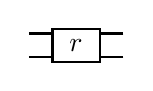
\begin{tikzpicture}[baseline=-.5ex,scale=0.6]
\draw[thick] (-1.5,-0.25) -- (-1,-0.25) (-1.5,0.25) -- (-1,0.25) (0.5,-0.25) -- (0,-0.25) (0.5,0.25) -- (0,0.25) (-1,-0.35) rectangle node {$r$} (0,0.35);
\end{tikzpicture}&=
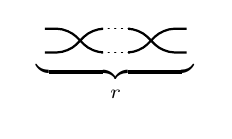
\begin{tikzpicture}[baseline=-.5ex,scale=0.6]
\draw[thick, rounded corners] (-1.5,0.25) -- (-1,0.25) -- (-0.5, -0.25) -- (-0.3, -0.25) (-1.5,-0.25) -- (-1,-0.25) -- (-0.5, 0.25) -- (-0.3, 0.25) (1.5,0.25) -- (1,0.25) -- (0.5, -0.25) -- (0.3, -0.25) (1.5,-0.25) -- (1,-0.25) -- (0.5, 0.25) -- (0.3, 0.25);
\draw[line cap=round, dotted] (-0.3,0.25) -- (0.3,0.25) (-0.3,-0.25) -- node[below] {$\underbrace{\hphantom{\hspace{2cm}}}_r$} (0.3,-0.25);
\end{tikzpicture}
\end{align*}

One can easily check the quiver $\quiver^{\mathsf{brick}}(\dynA_n)$ from the \emph{brick diagram} of $\beta_0(\dynA_n)$ described in \cite{GSW2020b} look as shown in Figure~\ref{figure:brick linear quiver}, and there is a canonical $N$-graph with cycles $(\ngraph^{\mathsf{brick}}(\dynA_n),\nbasis^{\mathsf{brick}}(\dynA_n))$ on $\disk^2$ as shown in Figure~\ref{figure:brick linear N-graph} such that 
\[
\quiver^{\mathsf{brick}}(\dynA_n)=
\quiver(\ngraph^{\mathsf{brick}}(\dynA_n), \nbasis^{\mathsf{brick}}(\dynA_n)).
\]
The colors on cycles in Figure~\ref{figure:brick linear N-graph} are nothing to do with the bipartite coloring.

\begin{figure}[ht]
\subfigure[Quiver $\quiver^{\mathsf{brick}}(\dynA_n)$\label{figure:brick linear quiver}]{$
\quiver^{\mathsf{brick}}(\dynA_n)=\begin{tikzpicture}[baseline=-.5ex, scale=1.2]
\draw[gray] (-3,0.25) -- (3,0.25) (-3,-0.25) -- (3,-0.25);
\foreach \i in {-2, -1, 0, 1, 2} {
\draw[gray] (\i, 0.25) -- (\i, -0.25) node[below] {$\sigma_1$};
}
\draw (0,-0.5) node[below] {$\underbrace{\hphantom{\hspace{4.8cm}}}_{n+1}$};
\node[Dnode] (A1) at (-1.5,0) {};
\node[Dnode] (A2) at (-0.5,0) {};
\node (A3) at (0.5,0) {$\cdots$};
\node[Dnode] (A4) at (1.5,0) {};
\draw[->] (A1) -- (A2);
\draw[->] (A2) -- (A3);
\draw[->] (A3) -- (A4);
\end{tikzpicture}
$}
\subfigure[$N$-graph $\ngraph^{\mathsf{brick}}(\dynA_n)$\label{figure:brick linear N-graph}]{$
(\ngraph^{\mathsf{brick}}(\dynA_n),\nbasis^{\mathsf{brick}}(\dynA_n))=
\begin{tikzpicture}[baseline=-.5ex,scale=1.2]
\draw[thick, rounded corners] (-3,-1) rectangle (2,1);
\begin{scope}
\clip (-3,-1) rectangle (2,1);
\draw[color=cyclecolor1, line cap=round, line width=5, opacity=0.5] (-2,0) -- (-1,0) (0.5,0) -- (1,0);
\draw[color=cyclecolor2, line cap=round, line width=5, opacity=0.5] (-1,0) -- (-0.5,0);
\draw[thick, blue] (-3,0) -- (-0.5, 0) (0.5,0) -- (2,0);
\foreach \x in {-2,-1,1} {
\draw[thick, blue, fill] (\x, -1) -- (\x,0) circle (1pt);
}
\draw[thick, blue, dashed] (-0.5,0) -- (0.5,0);
\end{scope}
\draw (-0.5, -1) node[below] {$\underbrace{\hphantom{\hspace{4cm}}}_{n+1}$};
\end{tikzpicture}
$}
\caption{Linear quiver $\quiver^{\mathsf{brick}}(\dynA_n)$ and $N$-graph $\ngraph^{\mathsf{brick}}(\dynA_n)$}
\label{figure:bricks linear}
\end{figure}

Then the quiver $\quiver^{\mathsf{brick}}(\dynA_n)$ is mutation equivalent to the bipartite quiver $\quiver(\dynA_n)$ as depicted in Figure~\ref{figure:linear quiver}.
\begin{figure}[ht]
\subfigure[Bipartite linear quivers $\quiver(\dynA_n)$ and $\quiver(\dynA_n)$\label{figure:linear quiver}]{\makebox[.45\textwidth]{$
\begin{tikzpicture}[baseline=-.5ex,xscale=-1]
\useasboundingbox (-1,-2.1) rectangle (2.1,2.1);
\draw (2,0) node[left] {$\quiver(\dynA_n)=$};
\node[Dnode, ynode] (A1) at (-1,0) {};
\node[Dnode, gnode] (A2) at (0,0) {};
\node[Dnode, ynode] (A3) at (1,0) {};
\node[Dnode] (A4) at (2,0) {};
\draw[<-] (A1) -- (A2);
\draw[->] (A2) -- (A3);
\draw[dotted] (A3) -- (A4);
\draw (0.5,-0.5) node {$\underbrace{\hphantom{\hspace{3cm}}}_n$};
\end{tikzpicture}
$}}
\subfigure[Linear $N$-graph $(\ngraph(\dynA_n),\nbasis(\dynA_n))$\label{figure:linear N-graph}]{\makebox[.45\textwidth]{$
\begin{tikzpicture}[baseline=-.5ex,xscale=0.6,yscale=0.6]
\useasboundingbox (-3.5,-3.5) rectangle (3.5,3.5);
\draw[thick] (0,0) circle (3);
\clip (0,0) circle (3);
\draw[color=cyclecolor2, line cap=round, line width=5, opacity=0.5] (-1.5,0.5) -- (-0.5, -0.5) node[midway, above,color=black,sloped,opacity=1] {$\cycle_2$}
	(1, 0) -- (1.5, -0.5);
\draw[color=cyclecolor1, line cap=round, line width=5, opacity=0.5] (-2.5,-0.5) -- (-1.5, 0.5) node[midway, above, color=black, sloped,opacity=1] {$\cycle_1$}
	(-0.5, -0.5) -- (0, 0) 
	(1.5, -0.5) -- (2.5, 0.5) node[midway, above, color=black, sloped,opacity=1] {$\cycle_n$};
\draw[blue, thick, fill] (0:3) -- (2.5,0.5) circle (2pt) -- (45:3) (2.5,0.5) -- (1.5,-0.5) circle (2pt) -- (-45:3) (1.5,-0.5) -- (1,0) (0.5,0) node {$\scriptstyle\cdots$} (0,0) -- (-0.5, -0.5) circle (2pt) -- (-90:3) (-0.5, -0.5) -- (-1.5, 0.5) circle (2pt) -- (135:3) (-1.5, 0.5) -- (-2.5, -0.5) circle (2pt) -- (-135:3);
\draw[blue, thick] (-2.5,-0.5) -- (-180:3);
\end{tikzpicture}
$}}
\caption{Bipartite linear quiver $\quiver(\dynA_n)$ and $N$-graph $(\ngraph(\dynA_n),\nbasis(\dynA_n))$ with chosen cycles}
\end{figure}


\begin{definition}[Linear $N$-graphs]
For $n\ge 1$, the \emph{linear $N$-graph} $(\ngraph(\dynA_n), \nbasis(\dynA_n))$ is the $2$-graph on $\disk^2$ depicted in Figure~\ref{figure:linear N-graph}, which satisfies that
\[
\quiver(\ngraph(\dynA_n), \nbasis(\dynA_n))=\quiver(\dynA_n).
\]
\end{definition}

It is easy but important to note that the $N$-graph $(\ngraph(\dynA_n),\nbasis(\dynA_n))$ has symmetries as follows:
\begin{lemma}
The $N$-graph $(\ngraph(\dynA_n),\nbasis(\dynA_n))$ with cycles is invariant under the conjugation.
Moreover, when $n$ is odd, it is invariant under $\pi$-rotation and the interchanges
\[
\cycle_i \leftrightarrow \cycle_{n+1-i}
\]
for cycles $\cycle_i\in \nbasis(\dynA_n)$.
\end{lemma}




\subsubsection{Tripod \texorpdfstring{$N$-graphs}{N-graphs}}\label{sec:tripods}
For $a,b,c\ge 1$, we define a Legendrian link $\legendrian(a,b,c)$, which is the closure of a braid $\beta(a,b,c)$
\begin{align*}
\legendrian(a,b,c) &= \legendrian_{\beta(a,b,c)},&
\beta(a,b,c)&=\sigma_2\sigma_1^{a+1}\sigma_2\sigma_1^{b+1}\sigma_2\sigma_1^{c+1},
\end{align*}
where $\beta(a,b,c)$ is equivalent to the following:
\begin{align*}
\beta(a,b,c)&=\sigma_2\sigma_1^{a+1}\sigma_2\sigma_1^{b+1}\sigma_2\sigma_1^{c+1}
=\sigma_2\sigma_1(\sigma_2\sigma_1)\sigma_2^a\sigma_1^{b-1}\sigma_2^c(\sigma_1\sigma_2)\sigma_1
=\Delta_3\sigma_1\sigma_2^a\sigma_1^{b-1}\sigma_2^c\Delta_3.
\end{align*}
Hence $\legendrian(a,b,c)$ in $J^1\sphere^1$ corresponds to the rainbow closure of the braid $\beta_0(a,b,c)=\sigma_1\sigma_2^a\sigma_1^{b-1}\sigma_2^c$.
\begin{align*}
&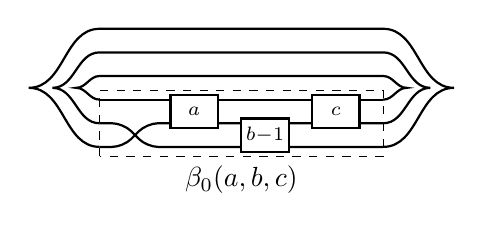
\begin{tikzpicture}[yshift=0.45cm,baseline=-.5ex,scale=0.6]
\draw[thick] (-3,-1)--(-1.5,-1) (-0.5,-1) -- (1.5, -1) (2.5,-1) -- (3,-1);
\draw[thick, rounded corners] (-3,-1.5) -- (-2.5,-1.5) -- (-2,-2) -- (0,-2) (-0.5,-1.5) -- (0, -1.5) (1, -1.5) -- (1.5,-1.5) (2.5, -1.5) -- (3,-1.5);
\draw[thick, rounded corners] (-3,-2) -- (-2.5,-2) -- (-2,-1.5) -- (-1.5,-1.5) (1,-2) -- (3,-2);
\draw[thick] (-1.5,-1.6) rectangle node {$\scriptstyle a$} (-0.5, -0.9) (0,-1.4) rectangle node {$\scriptstyle b-1$} (1,-2.1) (1.5,-0.9) rectangle node {$\scriptstyle c$} (2.5,-1.6);
\draw[thick] (-3,-1) to[out=180,in=0] (-3.5,-0.75) to[out=0,in=180] (-3,-0.5) -- (3,-0.5) to[out=0,in=180] (3.5,-0.75) to[out=180,in=0] (3,-1);
\draw[thick] (-3,-1.5) to[out=180,in=0] (-4,-0.75) to[out=0,in=180] (-3,0) -- (3,0) to[out=0,in=180] (4,-0.75) to[out=180,in=0] (3,-1.5);
\draw[thick] (-3,-2) to[out=180,in=0] (-4.5,-0.75) to[out=0,in=180] (-3,0.5) -- (3,0.5) to[out=0,in=180] (4.5,-0.75) to[out=180,in=0] (3,-2);
\draw[dashed] (-3,-2.2) rectangle (3,-0.8) (0,-2.2) node[below] {$\beta_0(a,b,c)$};
\end{tikzpicture}&
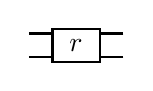
\begin{tikzpicture}[baseline=-.5ex,scale=0.6]
\draw[thick] (-1.5,-0.25) -- (-1,-0.25) (-1.5,0.25) -- (-1,0.25) (0.5,-0.25) -- (0,-0.25) (0.5,0.25) -- (0,0.25) (-1,-0.35) rectangle node {$r$} (0,0.35);
\end{tikzpicture}&=
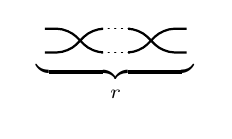
\begin{tikzpicture}[baseline=-.5ex,scale=0.6]
\draw[thick, rounded corners] (-1.5,0.25) -- (-1,0.25) -- (-0.5, -0.25) -- (-0.3, -0.25) (-1.5,-0.25) -- (-1,-0.25) -- (-0.5, 0.25) -- (-0.3, 0.25) (1.5,0.25) -- (1,0.25) -- (0.5, -0.25) -- (0.3, -0.25) (1.5,-0.25) -- (1,-0.25) -- (0.5, 0.25) -- (0.3, 0.25);
\draw[line cap=round, dotted] (-0.3,0.25) -- (0.3,0.25) (-0.3,-0.25) -- node[below] {$\underbrace{\hphantom{\hspace{2cm}}}_r$} (0.3,-0.25);
\end{tikzpicture}
\end{align*}

The quiver $\quiver^{\mathsf{brick}}(a,b,c)$ obtained from the brick diagram of $\beta_0(a,b,c)$ and the corresponding $N$-graph with cycles $(\ngraph^{\mathsf{brick}}(a,b,c),\nbasis^{\mathsf{brick}}(a,b,c))$ on $\disk^2$ are shown in Figure~\ref{figure:brick tripod N-graphs}.
That is, 
\begin{align*}
\quiver^{\mathsf{brick}}(a,b,c)&=
\quiver(\ngraph^{\mathsf{brick}}(a,b,c), \nbasis^{\mathsf{brick}}(a,b,c)).
\end{align*}
As before, the colors on cycles in Figure~\ref{figure:brick tripod N-graphs} are nothing to do with the bipartite coloring.

\begin{figure}[ht]
\subfigure[Quiver $\quiver^{\mathsf{brick}}(a,b,c)$\label{figure:brick tripod quiver}]{$
\quiver^{\mathsf{brick}}(a,b,c)=\begin{tikzpicture}[baseline=-.5ex,xscale=1.2, yscale=-1.2]
\draw[gray] (-5,0.5) -- (5,0.5) (-5,0) -- (5,0) (-5,-0.5) -- (5,-0.5);
\draw[gray] (-4.5,0) -- (-4.5,-0.5) node[above] {$\sigma_2$} (-4,0) -- (-4, 0.5) node[below] {$\sigma_1$} (-3.5, 0) -- (-3.5, 0.5) node[below] {$\sigma_1$} (-3, 0) -- (-3, 0.5) node[below] {$\sigma_1$} (-2.5,0.5) node[below] {$\cdots$} (-2,0) -- (-2,0.5) node[below] {$\sigma_1$} (-1.5,0) -- (-1.5,0.5) node[below] {$\sigma_1$};
\draw[gray] (-1,0) -- (-1, -0.5) node[above] {$\sigma_2$} (-0.5,0) -- (-0.5, -0.5) node[above] {$\sigma_2$} (0, 0) -- (0, -0.5) node[above] {$\sigma_2$} (0.5,-0.5) node[above] {$\cdots$} (1,0) -- (1,-0.5) node[above] {$\sigma_2$} (1.5,0) -- (1.5, -0.5) node[above] {$\sigma_2$};
\draw[gray] (2,0) -- (2,0.5) node[below] {$\sigma_1$} (2.5,0) -- (2.5,0.5) node[below] {$\sigma_1$} (3,0) -- (3,0.5) node[below] {$\sigma_1$} (3.5,0.5) node[below] {$\cdots$} (4,0) -- (4,0.5) node[below] {$\sigma_1$} (4.5,0) -- (4.5,0.5) node[below] {$\sigma_1$};
\draw (-2.75,0.5) node[yshift=-4ex] {$\underbrace{\hphantom{\hspace{3cm}}}_a$};
\draw (0.25,-0.5) node[yshift=4ex] {$\overbrace{\hphantom{\hspace{3cm}}}^{b-1}$};
\draw (3.25,0.5) node[yshift=-4ex] {$\underbrace{\hphantom{\hspace{3cm}}}_c$};
\node[Dnode] (A1) at (-3.75, 0.25) {};
\node[Dnode] (A2) at (-3.25, 0.25) {};
\node[Dnode] (A3) at (-1.75, 0.25) {};
\node[Dnode] (Aa) at (0.25, 0.25) {};
\node (Adots) at (-2.5,0.25) {$\cdots$};
\node[Dnode] (B1) at (2.25, 0.25) {};
\node[Dnode] (B2) at (2.75,0.25) {};
\node[Dnode] (Bb) at (4.25, 0.25) {};
\node (Bdots) at (3.5,0.25) {$\cdots$};
\node[Dnode] (C1) at (-2.75, -0.25) {};
\node[Dnode] (C2) at (-0.75, -0.25) {};
\node[Dnode] (C3) at (-0.25, -0.25) {};
\node[Dnode] (Cc) at (1.25, -0.25) {};
\node (Cdots) at (0.5, -0.25) {$\cdots$};
\draw[->] (A1) -- (A2);
\draw[->] (A2) -- (Adots);
\draw[->] (Adots) -- (A3);
\draw[->] (A3) -- (Aa);
\draw[->] (Aa) -- (B1);
\draw[->] (B1) -- (B2);
\draw[->] (B2) -- (Bdots);
\draw[->] (Bdots) -- (Bb);
\draw[->] (C1) -- (C2);
\draw[->] (C2) -- (C3);
\draw[->] (C3) -- (Cdots);
\draw[->] (Cdots) -- (Cc);
\draw[->] (Aa) -- (C1);
\end{tikzpicture}
$}
\subfigure[$N$-graph $\ngraph^{\mathsf{brick}}(a,b,c)$\label{figure:brick tripod N-graphs}]{$
(\ngraph^{\mathsf{brick}}(a,b,c),\nbasis^{\mathsf{brick}}(a,b,c))=
\begin{tikzpicture}[baseline=-.5ex,scale=1.2]
\draw[thick, rounded corners] (-4,-1) rectangle (3,1);
\begin{scope}
\clip (-4,-1) rectangle (3,1);
%
\draw[color=cyclecolor1, line cap=round, line width=5, opacity=0.5] (-3.5,0.5) -- (-1, 0.5) (-2.5,-0.5) -- (-2.25,-0.5) (-0.5, 0.5) -- (-0.25, 0.5) (1, -0.5) -- (1.5, -0.5) (2.25, -0.5) -- (2.5, -0.5);
\draw[color=cyclecolor2, line cap=round, line width=5, opacity=0.5] (-3,-0.5) -- (-2.5,-0.5) (-1.75, -0.5) -- (-1.5, -0.5) (-1, 0.5) -- (-0.5, 0.5) (0.25,0.5) -- (0.5,0.5) (1.5, -0.5) -- (1.75, -0.5);
\draw[color=cyan, line cap=round, line width=5, opacity=0.5] (-1, 0.5) -- (-1, -0.5)
(-1, -0.5) -- (1, -0.5)
(-0.5, 0.5) -- (-0.5, -0.5)
(0.5, -0.5) -- (0.5, 0.5)
 (-1.5,-0.5) -- (-1,-0.5);
%
\draw[thick, blue] 
(-4,-0.5) -- (-2.25, -0.5)
(-4, 0.5) -- (-0.25, 0.5)
(-1.75, -0.5) -- (-1,-0.5)
(-1, -0.5) -- (-0.25, -0.5)
(0.25, -0.5) -- (1.75,-0.5)
(0.25, 0.5) -- (3,0.5)
(2.25,-0.5) -- (3,-0.5);
%
\draw[thick, blue, fill] 
(-3.5, -0.5) -- (-3.5, 0.5) circle (1pt)
(-3, -1) -- (-3, -0.5) circle (1pt)
(-2.5, -1) -- (-2.5, -0.5) circle (1pt)
(-1.5,-1) -- (-1.5,-0.5) circle (1pt)
(-1, -0.5) -- (-1, 0.5) circle (1pt)
(-0.5, -0.5) -- (-0.5, 0.5) circle (1pt)
(0.5, -0.5) -- (0.5, 0.5) circle (1pt)
(1, -1) -- (1, -0.5) circle (1pt)
(1.5, -1) -- (1.5, -0.5) circle (1pt)
(2.5, -1) -- (2.5,-0.5) circle (1pt);
%
\draw[thick, blue, dotted]
(-2.25, -0.5) -- (-1.5, -0.5)
(-0.25, -0.5) -- (0.25, -0.5)
(-0.25, 0.5) -- (0.25, 0.5)
(1.75, -0.5) -- (2.25, -0.5);
%
\draw[thick, red] (-3.5,-1) -- (-3.5,-0.5) (-1, -1) -- (-1, -0.5) (-0.5,-1) -- (-0.5, -0.5) (0.5, -1) -- (0.5,-0.5);
\draw[thick, red, rounded corners] (-4,0) -- (-3.75,0) -- (-3.5,-0.5) (-3.5, -0.5) -- (-3.25, 0) -- (-1.25, 0) -- (-1, -0.5) 
(-1, -0.5) -- (-0.75, 0) -- (-0.5, -0.5) 
(-0.5, -0.5) -- (-0.25, 0) 
(0.25,0) -- (0.5,-0.5)
(0.5, -0.5) -- (0.75, 0) -- (1, 0) -- (3,0);
\draw[thick, red, dotted] (-0.25, 0) -- (0.25,0);
%
\foreach \x in {-3.5, -1, -0.5, 0.5} {
\draw[thick, fill=white] (\x,-0.5) circle (1pt) ;
}
\end{scope}
\draw (-2.25, -1) node[below] {$\underbrace{\hphantom{\hspace{2cm}}}_{a}$};
\draw (-.25, -1) node[below] {$\underbrace{\hphantom{\hspace{2cm}}}_{b-1}$};
\draw (1.75, -1) node[below] {$\underbrace{\hphantom{\hspace{2cm}}}_{c}$};
\end{tikzpicture}
$}
\caption{Tripod quiver $\quiver^{\mathsf{brick}}(a,b,c)$ and $N$-graph $\ngraph^{\mathsf{brick}}(a,b,c)$}
\label{figure:bricks tripod}
\end{figure}

This quiver $\quiver^{\mathsf{brick}}(a,b,c)$ is mutation equivalent to the quiver $\quiver(a,b,c)$, called the \emph{tripod quiver of type $(a,b,c)$}, depicted in Figure~\ref{figure:tripod quiver}.

\begin{definition}[Tripod $N$-graphs]
For $a,b,c\ge 1$, the \emph{tripod $N$-graph} $(\ngraph(a,b,c), \nbasis(a,b,c))$ is a free $3$-graph on $\disk^2$ depicted in Figure~\ref{figure:tripod N-graph}, which satisfies that
\[
\quiver(\ngraph(a,b,c), \nbasis(a,b,c))= \quiver(a,b,c).
\]
\end{definition}

\begin{figure}[ht]
\subfigure[Tripod quiver $\quiver(a,b,c)$\label{figure:tripod quiver}]{
\begin{tikzpicture}[baseline=-.5ex,scale=0.6]
\node[Dnode,ynode] (O) at (0,0) {};
\node[Dnode,gnode] (A1) at (60:1) {};
\node[Dnode,ynode] (A2) at (60:2) {};
\node[Dnode,gnode] (A3) at (60:3) {};
\node[Dnode] (An) at (60:4) {};
\node[Dnode,gnode] (B1) at (180:1) {};
\node[Dnode,ynode] (B2) at (180:2) {};
\node[Dnode,gnode] (B3) at (180:3) {};
\node[Dnode] (Bn) at (180:4) {};
\node[Dnode,gnode] (C1) at (-60:1) {};
\node[Dnode,ynode] (C2) at (-60:2) {};
\node[Dnode,gnode] (C3) at (-60:3) {};
\node[Dnode] (Cn) at (-60:4) {};
\draw[<-] (O)--(A1);
\draw[<-] (A2) --(A1);
\draw[<-] (A2)--(A3);
\draw[dotted] (A3) -- (An);
\draw[<-] (O)--(B1);
\draw[<-] (B2)--(B1);
\draw[<-] (B2)--(B3);
\draw[dotted] (B3)--(Bn);
\draw[<-] (O)--(C1);
\draw[<-] (C2)--(C1);
\draw[<-] (C2)--(C3);
\draw[dotted] (C3)--(Cn);
\draw (60:2.5) ++ (150:0.75) node[rotate=60]{$\overbrace{\hphantom{\hspace{1.8cm}}}^{a-1}$};
\draw (180:2.5) ++ (90:0.75) node[rotate=0]{$\overbrace{\hphantom{\hspace{1.8cm}}}^{b-1}$};
\draw (300:2.5) ++ (30:0.75) node[rotate=-60]{$\overbrace{\hphantom{\hspace{1.8cm}}}^{c-1}$};
\end{tikzpicture}
}
\subfigure[$(\ngraph(a,b,c), \nbasis(a,b,c))$\label{figure:tripod N-graph}]{
\begin{tikzpicture}[baseline=-.5ex,xscale=0.6,yscale=0.6]
\useasboundingbox(-3.5,-3.5)rectangle(3.5,3.5);
\draw[thick] (0,0) circle (3cm);
\draw[color=cyclecolor2, line cap=round, line width=5, opacity=0.5] (60:1) -- (50:1.5) (70:1.75) -- (50:2) (180:1) -- (170:1.5) (190:1.75) -- (170:2) (300:1) -- (290:1.5) (310:1.75) -- (290:2);
\draw[color=cyclecolor1, line cap=round, line width=5, opacity=0.5] (0,0) -- (60:1) (0,0) -- (180:1) (0,0) -- (300:1) (50:1.5) -- (70:1.75) (170:1.5) -- (190:1.75) (290:1.5) -- (310:1.75);
\draw[red, thick] (0,0) -- (0:3) (0,0) -- (120:3) (0,0) -- (240:3);
\draw[blue, thick, fill] (0,0) -- (60:1) circle (2pt) -- (100:3) (60:1) -- (50:1.5) circle (2pt) -- (20:3) (50:1.5) -- (70:1.75) circle (2pt) -- (80:3) (70:1.75) -- (50:2) circle (2pt) -- (40:3);
\draw[blue, thick, dashed] (50:2) -- (60:3);
\draw[blue, thick, fill] (0,0) -- (180:1) circle (2pt) -- (220:3) (180:1) -- (170:1.5) circle (2pt) -- (140:3) (170:1.5) -- (190:1.75) circle (2pt) -- (200:3) (190:1.75) -- (170:2) circle (2pt) -- (160:3);
\draw[blue, thick, dashed] (170:2) -- (180:3);
\draw[blue, thick, fill] (0,0) -- (300:1) circle (2pt) -- (340:3) (300:1) -- (290:1.5) circle (2pt) -- (260:3) (290:1.5) -- (310:1.75) circle (2pt) -- (320:3) (310:1.75) -- (290:2) circle (2pt) -- (280:3);
\draw[blue, thick, dashed] (290:2) -- (300:3);
\draw[thick, fill=white] (0,0) circle (2pt);
\curlybrace[]{10}{110}{3.2};
\draw (300:3.5) node[rotate=30] {$c+1$};
\curlybrace[]{130}{230}{3.2};
\draw (180:3.5) node[rotate=90] {$b+1$};
\curlybrace[]{250}{350}{3.2};
\draw (60:3.5) node[rotate=-30] {$a+1$};
\end{tikzpicture}
}
\subfigure[$\overline{(\ngraph(a,b,c), \nbasis(a,b,c))}$\label{figure:switched tripod N-graph}]{
\begin{tikzpicture}[baseline=-.5ex,xscale=0.6,yscale=0.6]
\useasboundingbox(-3.5,-3.5)rectangle(3.5,3.5);
\draw[thick] (0,0) circle (3cm);
\draw[color=cyclecolor2, line cap=round, line width=5, opacity=0.5] (60:1) -- (50:1.5) (70:1.75) -- (50:2) (180:1) -- (170:1.5) (190:1.75) -- (170:2) (300:1) -- (290:1.5) (310:1.75) -- (290:2);
\draw[color=cyclecolor1, line cap=round, line width=5, opacity=0.5] (0,0) -- (60:1) (0,0) -- (180:1) (0,0) -- (300:1) (50:1.5) -- (70:1.75) (170:1.5) -- (190:1.75) (290:1.5) -- (310:1.75);
\draw[blue, thick] (0,0) -- (0:3) (0,0) -- (120:3) (0,0) -- (240:3);
\draw[red, thick, fill] (0,0) -- (60:1) circle (2pt) -- (100:3) (60:1) -- (50:1.5) circle (2pt) -- (20:3) (50:1.5) -- (70:1.75) circle (2pt) -- (80:3) (70:1.75) -- (50:2) circle (2pt) -- (40:3);
\draw[red, thick, dashed] (50:2) -- (60:3);
\draw[red, thick, fill] (0,0) -- (180:1) circle (2pt) -- (220:3) (180:1) -- (170:1.5) circle (2pt) -- (140:3) (170:1.5) -- (190:1.75) circle (2pt) -- (200:3) (190:1.75) -- (170:2) circle (2pt) -- (160:3);
\draw[red, thick, dashed] (170:2) -- (180:3);
\draw[red, thick, fill] (0,0) -- (300:1) circle (2pt) -- (340:3) (300:1) -- (290:1.5) circle (2pt) -- (260:3) (290:1.5) -- (310:1.75) circle (2pt) -- (320:3) (310:1.75) -- (290:2) circle (2pt) -- (280:3);
\draw[red, thick, dashed] (290:2) -- (300:3);
\draw[thick, fill=white] (0,0) circle (2pt);
\curlybrace[]{10}{110}{3.2};
\draw (-60:3.5) node[rotate=30] {$c+1$};
\curlybrace[]{130}{230}{3.2};
\draw (180:3.5) node[rotate=90] {$b+1$};
\curlybrace[]{250}{350}{3.2};
\draw (-300:3.5) node[rotate=-30] {$a+1$};
\end{tikzpicture}
}
\caption{Tripod quiver and $N$-graphs with chosen cycles}
\label{figure:tripod}
\end{figure}

Moreover, the above two $N$-graphs are essentially equivalent as follows.
The proof will be given in Appendix~\ref{appendix:Ngraph of type abc}.
\begin{lemma}
The $N$-graphs $\ngraph^{\mathsf{brick}}(a,b,c)$ and $\ngraph(a,b,c)$ are equivalent up to $\boundary$-Legendrian isotopy and Legendrian mutations.
\end{lemma}

The $N$-graph $\ngraph(a,b,c)$ is free by Lemma~\ref{lemma:tree Ngraphs are free} and is never invariant under the conjugation, which acts on the Legendrian $\legendrian(a,b,c)$ as interchanging $\sigma_1$ and $\sigma_2$ so that $\overline{\legendrian(a,b,c)}$ is the closure of $\overline{\beta(a,b,c)}$
\[
\overline{\beta(a,b,c)} = \sigma_1\sigma_2^{a+1}\sigma_1\sigma_2^{b+1}\sigma_1\sigma_2^{c+1}.
\]
The conjugation $\overline{(\nbasis(a,b,c),\nbasis(a,b,c))}$ is depicted in Figure~\ref{figure:switched tripod N-graph}.

We have the following obvious observation:
\begin{lemma}
For each $a\ge 1$, the $N$-graph $\ngraph(a,a,a)$ is invariant under $2\pi/3$-rotation.
\end{lemma}

On the other hand, if one of $a,b,c$ is $1$, then the quiver $\quiver(a,b,c)$ is of type $\dynA_n$. Indeed, 
as seen in Example~\ref{example:stabilization of An}, the Legendrian link $\legendrian(1,b,c)$ is a stabilization of $\legendrian(\dynA_n)$ for $n=b+c-1$, and the $N$-graph $\ngraph(a,b,c)$ is a stabilization of $\ngraph(\dynA_n)$.
See Appendix~\ref{appendix:tripod with a=1 is of type An} for the proof.
\begin{lemma}\label{lemma:stabilized An}
The $N$-graph $\ngraph(1,b,c)$ is a stabilization of $\ngraph(\dynA_n)$ for $n=b+c-1$.
\end{lemma}
One consequence of this lemma is that two $N$-graphs $\ngraph(\dynA_n)$ and $\ngraph(1,b,c)$ with $n=b+c-1$ will generate bijective sets of $N$-graphs under mutations as seen in Remarks~\ref{remark:boundary-Legendrian isotopy} and \ref{remark:Stabilization}, where the bijection preserves the mutation.

Notice that the quivers $\quiver(a,b,c)$ together with $\quiver(\dynA_n)$ cover all quivers of finite type and some quivers of affine type. Indeed, for $1\le a\le b\le c$ and $n=a+b+c-2$, the quivers $\quiver(1,b,c)$ and $\quiver(\dynA_n)$ are of type $\dynA_n$, and the quivers $\quiver(2,2,n-2)$ and $\quiver(2,3,n-3)$ are of type $\dynD_n$ and $\dynE_n$.
Moreover, $\quiver(3,3,3)$, $\quiver(2,4,4)$ and $\quiver(2,3,6)$ are of type $\exdynE_6, \exdynE_7$ and $\exdynE_8$, respectively.
Hence as seen in Table~\ref{table:short notations}, we denote braids, Legendrians, quivers, and $N$-graphs with cycles by $\beta(\dynX)$, $\legendrian(\dynX)$, $\quiver(\dynX)$ and $\ngraph(\dynX)$ for $\dynX=\dynD_n, \dynE_n$ or $\exdynE_n$, respectively.

\begin{table}[ht]
\[
\renewcommand\arraystretch{1.5}
\begin{array}{c||c|c|c|c}
\toprule
\dynX & \beta(\dynX) & \legendrian(\dynX) & \quiver(\dynX) & (\ngraph(\dynX), \nbasis(\dynX))\\
\midrule
%\hline
%\dynA_n, n=b+c-1\ge 1 & \beta(1,b,c) & \legendrian(1,b,c) & \quiver(1,b,c) & (\ngraph(1,b,c),\nbasis(1,b,c))\\
%\hline
\dynD_n, n\ge 4 & \beta(n-2,2,2) & \legendrian(n-2,2,2) & \quiver(n-2,2,2) & (\ngraph(n-2,2,2),\nbasis(n-2,2,2))\\
\hline
\dynE_6 & \beta(2,3,3) & \legendrian(2,3,3) & \quiver(2,3,3) & (\ngraph(2,3,3),\nbasis(2,3,3))\\
\hline
\dynE_7 & \beta(2,3,4) & \legendrian(2,3,4) & \quiver(2,3,4) & (\ngraph(2,3,4),\nbasis(2,3,4))\\
\hline
\dynE_8 & \beta(2,3,5) & \legendrian(2,3,5) & \quiver(2,3,5) & (\ngraph(2,3,5),\nbasis(2,3,5))\\
\hline
\exdynE_6 & \beta(3,3,3) & \legendrian(3,3,3) & \quiver(3,3,3) & (\ngraph(3,3,3),\nbasis(3,3,3))\\
\hline
\exdynE_7 & \beta(2,4,4) & \legendrian(2,4,4) & \quiver(2,4,4) & (\ngraph(2,4,4),\nbasis(2,4,4))\\
\hline
\exdynE_8 & \beta(2,3,6) & \legendrian(2,3,6) & \quiver(2,3,6) & (\ngraph(2,3,6),\nbasis(2,3,6))\\
\bottomrule
\end{array}
\]
\caption{Braids, Legendrians, quivers, and $N$-graphs of type $\dynD\dynE$ and $\exdynE$}
\label{table:short notations}
\end{table}


\subsubsection{Degenerate $N$-graphs of type $\dynD_{n+1}, \dynE_6, \exdynE_6$ and $\exdynE_7$}
For $a, b\ge 1$, we define positive braids $\tilde\beta_0(a,b,b)$ and $\tilde\beta(a,b,b)$ as follows:
\begin{align*}
\tilde\beta_0(a,b,b)&\colonequals \sigma_2^a\sigma_{1,3}^{b-1}\sigma_2\sigma_{1,3}
\mathrel{\dot{=}}\sigma_1\sigma_2^a \sigma_1^{b-1} \sigma_3^{b-1}\sigma_2\sigma_3
=\sigma_1\sigma_2^a \sigma_1^{b-1}\sigma_2{\color{blue}\sigma_3} \sigma_2^{b-1}
=S(\beta_0(a,b,b))\\
\tilde\beta(a,b,b)&\colonequals \sigma_2^{a+1}\sigma_{1,3}\sigma_2\sigma_{1,3}^{b}\sigma_2^2\sigma_{1,3}\sigma_2\sigma_{1,3}^2\\
&=\2^a(\2 \5 \2) \5^b (\2 \5)^3 \\
&=\2^a \5^{b-1} \2 \5 (\2 \5)^2 (\2 \5)^2 \\
&\mathrel{\dot{=}}\Delta_4\tilde\beta_0(a,b,b)\Delta_4.
\end{align*}

Let $\tilde\legendrian(a,b,b)$ be the closure of $\tilde\beta(a,b,b)$.
Then since both $\tilde\beta_0(a,b,b)$ and $\tilde\beta(a,b,b)$ are invariant under the conjugation, so is $\tilde\legendrian(a,b,b)$.

The quiver $\quiver^{\mathsf{brick}}(\tilde\beta_0(a,b,b))$ and $N$-graph $\tilde\ngraph^{\mathsf{brick}}(a,b,b)$ look as follows:
\begin{align*}
\quiver^{\mathsf{brick}}(\tilde\beta_0(a,b,b)))&=\begin{tikzpicture}[baseline=-.5ex,xscale=1.2, yscale=1.2]
\draw[gray] (-5,0.75) -- ++(7.5,0) (-5,0.25) -- ++(7.5,0);
\draw[gray] (-5,-0.75) -- ++(7.5,0) (-5,-0.25) -- ++(7.5,0);
%
\draw[gray] (-1.5,0.75) node[above] {$\sigma_3$} -- ++(0,-0.5) (-1,0.75) node[above] {$\sigma_3$} -- ++(0,-0.5) (-0.5,0.75) node[above] {$\sigma_3$} -- ++(0,-0.5) (0.5,0.75) node[above] {$\sigma_3$} -- ++(0,-0.5) (1,0.75) node[above] {$\sigma_3$} -- ++(0,-0.5) (2,0.75) node[above] {$\sigma_3$} -- ++(0,-0.5);
%
\draw[gray] (-1.5,-0.75) node[below] {$\sigma_1$} -- ++(0,0.5) (-1,-0.75) node[below] {$\sigma_1$} -- ++(0,0.5) (-0.5,-0.75) node[below] {$\sigma_1$} -- ++(0,0.5) (0.5,-0.75) node[below] {$\sigma_1$} -- ++(0,0.5) (1,-0.75) node[below] {$\sigma_1$} -- ++(0,0.5) (2,-0.75) node[below] {$\sigma_1$} -- ++(0,0.5);
%
\draw[gray] (-4.5,0.25) node[above] {$\sigma_2$} -- ++(0,-0.5) (-4,0.25) node[above] {$\sigma_2$} -- ++(0,-0.5) (-3.5,0.25) node[above] {$\sigma_2$} -- ++(0,-0.5) (-2.5,0.25) node[above] {$\sigma_2$} -- ++(0,-0.5) (-2,0.25) node[above] {$\sigma_2$} -- ++(0,-0.5) (1.5,0.25) -- ++(0,-0.5);
\node[Dnode] (A1) at (-4.25, 0) {};
\node[Dnode] (A2) at (-3.75, 0) {};
\node (Adots) at (-3, 0) {$\cdots$};
\node[Dnode] (A3) at (-2.25, 0) {};
\node[Dnode] (A4) at (0.75, 0) {};
\node[Dnode] (B1) at (-1.25,0.5) {};
\node[Dnode] (C1) at (-1.25,-0.5) {};
\node[Dnode] (B2) at (-.75,0.5) {};
\node[Dnode] (C2) at (-.75,-0.5) {};
\node (Bdots) at (0,0.5) {$\cdots$};
\node (Cdots) at (0,-0.5) {$\cdots$};
\node[Dnode] (B3) at (0.75,0.5) {};
\node[Dnode] (C3) at (0.75,-0.5) {};
\node[Dnode] (B4) at (1.5,0.5) {};
\node[Dnode] (C4) at (1.5,-0.5) {};
\draw[->] (A1) -- (A2);
\draw[->] (A2) -- (Adots);
\draw[->] (Adots) -- (A3);
\draw[->] (A3) -- (A4);
\draw[->] (B1) -- (B2);
\draw[->] (C1) -- (C2);
\draw[->] (B2) -- (Bdots);
\draw[->] (C2) -- (Cdots);
\draw[->] (Bdots) -- (B3);
\draw[->] (Cdots) -- (C3);
\draw[->] (B3) -- (B4);
\draw[->] (C3) -- (C4);
\draw[->] (B4) -- (A4);
\draw[->] (C4) -- (A4);
\end{tikzpicture}
\\
\tilde\ngraph^{\mathsf{brick}}(a,b,b)&=
\begin{tikzpicture}[baseline=-.5ex, scale=0.6]
\draw[rounded corners=5,thick] (-7, -2.5) rectangle (7, 2.5);
\draw (-4.5, -2.5) node[below] {$\underbrace{\hphantom{\hspace{2.4cm}}}_{a}$};
\draw (0.5, -2.5) node[below] {$\underbrace{\hphantom{\hspace{2.4cm}}}_{b-1}$};
\clip[rounded corners=5] (-7, -2.5) rectangle (7, 2.5);
\draw[thick, red, rounded corners] (-7, 0.5) -- ++(4, 0) -- ++(2, -1) -- ++(3, 0) -- ++(2, 1) -- ++(2, -1) -- ++(1,0);
%
\draw[thick, red, rounded corners] (-7, -1.5) -- ++(4, 0) ++(0,0) -- ++(2, 3) -- ++(3,0) -- ++(2,-3) ++(0,0) -- ++(2,3) -- ++(1,0);
\draw[thick, red, fill] 
(-7, -1.5) ++(1,0) circle (2pt) -- +(0,-1) 
++(1,0) circle (2pt) -- +(0,-1)
++(2,0) circle (2pt) -- +(0,-1)
++(7,0) circle (2pt) -- +(0,-1)
;
\draw (-7, -2) ++(3,0) node {$\cdots$};
%
\draw[Dble={green and blue},line width=2, line cap=round] (-7,-0.5) -- ++(4,0);
\draw[Dble={green and blue},line width=2, line cap=round] (-3,-0.5) -- ++(1,0.5);
\draw[Dble={blue and green},line width=2, line cap=round] (-2,0) -- (-1,0.5);
\draw[Dble={blue and green},line width=2, line cap=round] (-1,0.5) -- ++(3,0);
\draw[Dble={green and blue},line width=2, line cap=round] (3,0) -- ++(1,-0.5);
\draw[Dble={blue and green},line width=2, line cap=round] (2,0.5) -- ++(1,-0.5);
\draw[Dble={green and blue},line width=2, line cap=round] (3,0) -- ++(1,-0.5);
\draw[Dble={green and blue},line width=2, line cap=round] (4,-0.5) -- ++(1,0.5);
\draw[Dble={blue and green},line width=2, line cap=round] (5,0) -- ++(1,0.5);
\draw[Dble={blue and green},line width=2, line cap=round] (6,0.5) -- ++(1,0);
\draw[Dble={blue and green},line width=2, line cap=round] (-7,1.5) -- ++(4,0);
\draw[Dble={blue and green},line width=2, line cap=round] (-3,1.5) -- ++(1,-1.5);
\draw[Dble={green and blue},line width=2] (-2,0) -- ++(1,-1.5);
\draw[Dble={green and blue},line width=2, line cap=round] (-1,-1.5) -- ++(3,0);
\draw[Dble={green and blue},line width=2] (-1,-1.5) -- ++(0,-1);
\draw[Dble={green and blue},line width=2] (0,-1.5) -- ++(0,-1);
\draw[Dble={green and blue},line width=2] (2,-1.5) -- ++(0,-1);
\draw[Dble={green and blue},line width=2] (2,-1.5) -- ++(1,1.5);
\draw[Dble={blue and green},line width=2, line cap=round] (3,0) -- ++(1,1.5);
\draw[Dble={blue and green},line width=2, line cap=round] (4,1.5) -- ++(1,-1.5);
\draw[Dble={green and blue},line width=2] (5,0) -- ++(1,-1.5);
\draw[Dble={green and blue},line width=2] (6,-1.5) -- ++(1,0);
\draw[Dble={green and blue},line width=2, line cap=round] (6,-1.5) -- ++(0,-1);
\draw (1, -2) node {$\cdots$};
\end{tikzpicture}\\
&\stackrel{\rm perturb}{\rightarrow}
\begin{tikzpicture}[baseline=-.5ex, scale=0.6]
\draw[rounded corners=5,thick] (-7, -2.5) rectangle (7, 2.5);
\clip[rounded corners=5] (-7, -2.5) rectangle (7, 2.5);
\draw[color=cyclecolor1, line cap=round, line width=5, opacity=0.5, rounded corners]
(-6,-1.5) -- (-5,-1.5) (-3.5,-1.5)--(-3,-1.5) (-1,-1.5)--(0,-1.5) (2,-1.5)--(2.5,-0.5)--(2.5,0.5)--(4,1.5)--(5.5,0.5) -- (5.5,-0.5) -- (6,-1.5) 
(-1.5,-2)--(-0.5,-2) (1.5,-2)--(2.5,-2)--(3.5,-0.5)--(3.5,0.5)--(4,1)--(4.5,0.5)--(4.5,-0.5)--(5.5,-2);
\draw[color=cyclecolor2, line cap=round, line width=5, opacity=0.5, rounded corners]
(-5,-1.5)--(-4.5,-1.5) (0,-1.5)--(0.5,-1.5) (1.5,-1.5)--(2,-1.5) (-0.5,-2)--(0,-2) (1,-2)--(1.5,-2)
(-3,-1.5)--(-2.5,-0.5)--(-1.5,0.5)--(-1,1.5)--(2,1.5)--(2.5,0.5)--(3.5,-0.5)--(4,-1.5);
\draw[thick, blue, rounded corners] 
(-7,2) -- (-2.5,2) -- (-1.5,0.5) (2.5, 0.5) -- (4,1.5) -- (5.5,0.5) (1.5,-2)--(2.5,-2)--(3.5,-0.5);
\draw[thick, blue] 
(-7,-0.5) -- (-2.5,-0.5) -- (-1.5,-2) --(1.5,-2)  (3.5,-0.5) -- (4.5,-0.5) -- (5.5,-2) -- (7,-2)
(-2.5,-0.5) -- (-1.5,0.5) -- (2.5,0.5) -- (3.5,-0.5) (4.5,-0.5) -- (5.5,0.5) -- (7,0.5)
(-1.5,-2) -- (-1.5,-2.5) (-0.5,-2) -- (-0.5,-2.5) (1.5,-2) -- (1.5,-2.5) (5.5,-2) -- (5.5,-2.5) ;
\draw[thick, red, rounded corners] 
(-1.5,0.5) -- (-1,1.5) -- (2,1.5) -- (2.5,0.5) (5.5,0.5)-- (6,1.5) -- (7,1.5)
(-1.5,-0.5) -- (-1,-1) -- (2,-1) -- (2.5,-0.5) (5.5,-0.5)-- (6,-1) -- (7,-1);
\draw[thick, red] 
(-7,0.5) -- (-1.5,0.5) (2.5,0.5) -- (5.5,0.5) (-7,-1.5) -- (-3,-1.5) -- (-2.5,-0.5) -- (-1.5,-0.5)
(2.5,-0.5) -- (3.5,-0.5) -- (4,-1.5) -- (4.5,-0.5) -- (5.5,-0.5)
(-6,-1.5) -- (-6,-2.5) (-5,-1.5) -- (-5,-2.5)(-3,-1.5) -- (-3,-2.5)
(-2.5,0.5)--(-2.5,-0.5) (-1.5,0.5)-- (-1.5,-0.5)
(2.5,0.5)--(2.5,-0.5) (3.5,0.5)-- (3.5,-0.5)
(4.5,0.5)--(4.5,-0.5) (5.5,0.5)-- (5.5,-0.5) (4,-1.5) -- (4,-2.5);
\draw[thick, green, rounded corners] 
(-7,1.5) -- (-3,1.5) -- (-2.5,0.5) (-7,0)-- (-3,0) -- (-2.5,0.5) (3.5,0.5)--(4,1)--(4.5,0.5);
\draw[thick, green]
(-2.5,0.5)--(-1.5,-0.5) -- (2.5,-0.5) -- (3.5,0.5) (4.5,0.5)--(5.5,-0.5)--(7,-0.5)
(-1.5,-0.5) -- (-1,-1.5) -- (2,-1.5) -- (2.5,-0.5) (5.5,-0.5)--(6,-1.5) --(7,-1.5)
(-1,-1.5)--(-1,-2.5) (0,-1.5)--(0,-2.5) (2,-1.5)--(2,-2.5) (6,-1.5)--(6,-2.5);
\draw[thick, blue, fill] 
(-1.5,-2) circle (2pt) (-0.5,-2) circle (2pt) (1.5,-2) circle (2pt) (5.5,-2) circle (2pt) ;
\draw[thick, red, fill] 
(-6,-1.5) circle (2pt) (-5,-1.5) circle (2pt) (-3,-1.5) circle (2pt) (4,-1.5) circle (2pt) ;
\draw[thick, green, fill] 
(-1,-1.5) circle (2pt) (0,-1.5) circle (2pt) (2,-1.5) circle (2pt) (6,-1.5) circle (2pt) ;
\draw[fill=white, thick] 
(-2.5,0.5) circle (2pt) (-1.5,0.5) circle (2pt) (2.5,0.5) circle (2pt) (3.5,0.5) circle (2pt)
(4.5,0.5) circle (2pt) (5.5,0.5) circle (2pt)
(-2.5,-0.5) circle (2pt) (-1.5,-0.5) circle (2pt) (2.5,-0.5) circle (2pt) (3.5,-0.5) circle (2pt)
(4.5,-0.5) circle (2pt) (5.5,-0.5) circle (2pt);
\end{tikzpicture}
\end{align*}

\begin{definition}[Degenerate $4$-graphs for $\tilde\legendrian(a,b,b)$]
We define a degenerate $4$-graph $\tilde\ngraph(a,b,b)$ for $\tilde\legendrian(a,b,b)$ as depicted in the left of Figure~\ref{figure:degenerated 4-graph}.
\end{definition}

\begin{figure}[ht]
\[
\begin{tikzcd}[ampersand replacement=\&]
\tilde\ngraph(a,b,b)\colonequals
\begin{tikzpicture}[baseline=-.5ex, scale=0.8]
\draw (0,0) circle (3);
\curlybrace[]{200}{250}{3.2};
\draw (225:3.5) node[rotate=-45] {$a+1$};
\curlybrace[]{-30}{30}{3.2};
\draw (0:3.5) node[rotate=-90] {$b$};
%
\clip (0,0) circle (3);
\draw[fill, red, thick]
(3,-3) -- (0,0) 
(0,0) -- (-3,3)
(0,0) -- (45:2.5) circle (2pt)
(45:2.5) -- ++(0,3) (45:2.5) -- ++(3,0)
(0,0) -- (-135:1.5) circle (2pt)
(-135:1.5) -- ++(0,-3)
(-135:1.5) -- ++(-3,0)
(-135:1.5) ++ (-.5,0) circle (2pt) -- ++(0,-2)
(-135:1.5) ++ (-.5,-.5) circle (2pt) -- ++(-2,0)
(-135:1.5) ++ (-1,-.5) circle (2pt);
\draw[red, thick, dashed]
(-135:1.5) ++ (-1,-.5) -- ++(0,-2);
%
\draw[Dble={green and blue},line width=2] (-2.5,0) -- ++(-1,-1);
\draw[Dble={green and blue},line width=2] (-2.5,0) -- ++(-1,1);
\draw[Dble={blue and green},line width=2] (-2.5,0) -- (0,0);
\draw[Dble={blue and green},line width=2] (0,0) -- (0,3);
\draw[Dble={blue and green},line width=2] (0,0) -- (0,-3);
\draw[Dble={green and blue},line width=2] (0,0) -- (1.25,0);
\draw[Dble={green and blue},line width=2] (1.25,0) -- ++(2,-2);
\draw[Dble={green and blue},line width=2] (1.25,0) -- ++(2,2);
\draw[Dble={green and blue},line width=2] (1.25,0) ++(45:0.5) -- ++(2,-2);
\draw[Dble={green and blue},line width=2,dashed] (1.25,0) ++(45:0.5) ++(-45:0.5) -- ++(2,2);
%
\end{tikzpicture}\arrow[r,"\text{Perturb.}"] \&
\begin{tikzpicture}[baseline=-.5ex, scale=0.8]
\draw (0,0) circle (3);
\clip (0,0) circle (3);
\draw[cyclecolor1, opacity=0.5, line width=5, line cap=round] 
(-2.5,0.25) -- (1.25, 0.25) (-2.5,-0.25) -- (1.25, -0.25)
(1.25, 0.25) ++(45:0.5) -- ++(-45:0.5) (1.25, -0.25) ++(45:0.5) -- ++(-45:0.5)
(-135:1.5) -- ++(-0.5,0)
(-135:1.5) ++(-0.5,-0.5) -- ++(-0.5,0)
;
\draw[cyclecolor2, opacity=0.5, line width=5, line cap=round] 
(1.25, 0.25) -- ++(45:0.5) (1.25, -0.25) -- ++(45:0.5)
(45:2.5) -- (-135:1.5)
(-135:1.5) ++(-0.5,0) -- ++(0,-0.5)
;
\draw[fill, red, thick]
(3,-3) -- (0.25,-0.25) 
(-0.25,0.25) -- (-3,3)
(0.25,0.25) -- (45:2.5) circle (2pt)
(45:2.5) -- ++(0,3) (45:2.5) -- ++(3,0)
(-0.25,-0.25) -- (-135:1.5) circle (2pt)
(-135:1.5) -- ++(0,-3)
(-135:1.5) -- ++(-3,0)
(-135:1.5) ++ (-.5,0) circle (2pt) -- ++(0,-2)
(-135:1.5) ++ (-.5,-.5) circle (2pt) -- ++(-2,0)
(-135:1.5) ++ (-1,-.5) circle (2pt);
\draw[red, thick] (-0.25,-0.25) rectangle (0.25,0.25);
\draw[red, thick, dashed]
(-135:1.5) ++ (-1,-.5) -- ++(0,-2);
%
\draw[green, thick, fill] (-2.5,-0.25) circle (2pt) -- ++(-1,-1);
\draw[green, thick] (-2.5,-0.25) -- ++(-1,1);
\draw[green, thick] (-2.5,-0.25) -- (-0.25,-0.25) -- ++(0,-3);
\draw[blue, thick, fill] (-2.5,0.25) circle (2pt) -- ++(-1,-1);
\draw[blue, thick] (-2.5,0.25) -- ++(-1,1);
\draw[blue, thick] (-2.5,0.25) -- (-0.25,0.25) -- ++(0,3);
%
\draw[green, thick] (0.25, 0.25) -- (-0.25, -0.25);
\draw[green, thick, fill] (0.25,0.25) -- ++(0,3);
\draw[green, thick, fill] (0.25,0.25) -- ++(1,0);
\draw[green, thick, fill] (1.25,0.25) circle (2pt) -- ++(2,-2);
\draw[green, thick, fill] (1.25,0.25) -- ++(2,2);
\draw[green, thick, fill] (1.25,0.25) ++(45:0.5) circle (2pt) -- ++(2,-2);
\draw[green, thick, fill, dashed] (1.25,0.25) ++(45:0.5) ++(-45:0.5) circle (2pt) -- ++(2,2);
%
\draw[blue, thick] (-0.25, 0.25) -- (0.25, -0.25);
\draw[blue, thick, fill] (0.25,-0.25) -- ++(1,0);
\draw[blue, thick, fill] (0.25,-0.25) -- ++(0,-3);
\draw[blue, thick, fill] (1.25,-0.25) circle (2pt) -- ++(2,-2);
\draw[blue, thick, fill] (1.25,-0.25) -- ++(2,2);
\draw[blue, thick, fill] (1.25,-0.25) ++(45:0.5) circle (2pt) -- ++(2,-2);
\draw[blue, thick, fill, dashed] (1.25,-0.25) ++(45:0.5) ++(-45:0.5) circle (2pt) -- ++(2,2);
%
\draw[fill=white, thick] (0.25, 0.25) circle (2pt) (0.25, -0.25) circle (2pt) (-0.25, -0.25) circle (2pt) (-0.25, 0.25) circle (2pt);
\end{tikzpicture}
\end{tikzcd}
\]
\caption{Degenerate $4$-graphs $\tilde\ngraph(a,b,b)$ and cycles in the perturbation}
\label{figure:degenerated 4-graph}
\end{figure}

\begin{lemma}\label{lemma:tripod to degenerated Ngraph}
The $N$-graph $\tilde\ngraph(a,b,b)$ is equivalent to $\tilde\ngraph^{\mathsf{brick}}(a,b,b)$ up to $\boundary$-Legendrian isotopy and Legendrian mutations.
\end{lemma}
\begin{proof}
It is straightforward to check that we obtain the following degenerate $N$-graph from $\tilde\ngraph^{\mathsf{brick}}(a,b,b)$ by applying a sequence of Move \Move{DI}.
\[
\begin{tikzpicture}[baseline=-.5ex, scale=0.6]
\draw[rounded corners=5,thick] (-7, -2.5) rectangle (7, 2.5);
\clip[rounded corners=5] (-7, -2.5) rectangle (7, 2.5);
\draw[red, thick, rounded corners]
(-7,0.5) -- (-3.5,0.5) (-2.5,0.5)--(-2,0.5)
(-7,-1.5)--(-6,-0.5)--(-6,2)--(-3.5,2) (-2.5,2)--(3,2)--(3,0.5)
(-2,0.5)--(-1,-0)--(2,0)--(4,1)--(5,0.5)
(5,0.5)--(5.5,1)--(6,0.5)
(5,0.5)--(5.5,0)--(6,0.5)
(-6,-2.5)--(-5,-1.5)--(-5,2)
(-5,-2.5)--(-4,-1.5)--(-4,2)
(-3,-2.5)--(-2,-1.5)--(-2,2);
\draw[red, thick, dashed]
(-3.5,0.5)--(-2.5,0.5) (-3.5,2)--(-2.5,2);
\draw[red, thick]
(3,0.5)--(4,-1.5)--(5,0.5) (7,1)--(6,0.5)--(7,-0.5)
(4,-1.5)--(4,-2.5);
\draw[Dble={blue and green},line width=2] (5,0.5)--(5.5,0.5);
\draw[Dble={green and blue},line width=2] (5.5,0.5)--(6,0.5);
\draw[Dble={green and blue},line width=2, line cap=round] (-6,0.5)--(-5.5,0);
\draw[Dble={blue and green},line width=2, line cap=round] (-6,0.5)--(-5.5,1);
\draw[Dble={green and blue},line width=2, line cap=round] (-5,0.5)--(-4.5,0);
\draw[Dble={blue and green},line width=2, line cap=round] (-5,0.5)--(-4.5,1);
\draw[Dble={green and blue},line width=2, line cap=round] (-4,0.5)--(-3.5,0);
\draw[Dble={blue and green},line width=2, line cap=round] (-4,0.5)--(-3.5,1);
\draw[Dble={green and blue},line width=2, line cap=round] (-2,0.5)--(-1,-1.5);
\draw[Dble={blue and green},line width=2, line cap=round] (-2,0.5)--(-1,1);
\draw[Dble={blue and green},line width=2, line cap=round] (3,0.5)--(4,2);
\draw[Dble={green and blue},line width=2, line cap=round] (4,0)--(5,0.5);
\draw[Dble={green and blue},line width=2] (5,0.5)--(5.5,2);
\draw[Dble={green and blue},line width=2] (3,0.5)--(4,0);
\draw[Dble={blue and green},line width=2] (-7,1.5)--(-6,0.5);
\draw[Dble={green and blue},line width=2] (-7,-0.5)--(-6,0.5);
\draw[Dble={green and blue},line width=2] (-5.5,0)--(-5,0.5);
\draw[Dble={blue and green},line width=2] (-5.5,1)--(-5,0.5);
\draw[Dble={green and blue},line width=2] (-4.5,0)--(-4,0.5);
\draw[Dble={blue and green},line width=2] (-4.5,1)--(-4,0.5);
\draw[Dble={green and blue},line width=2] (-2.5,0)--(-2,0.5);
\draw[Dble={blue and green},line width=2] (-2.5,1)--(-2,0.5);
\draw[Dble={blue and green},line width=2, line cap=round] (4,2)--(5.5,2);
\draw[Dble={blue and green},line width=2] (5.5,2)--(6,0.5);
\draw[Dble={blue and green},line width=2] (6,0.5)--(7,0.5);
\draw[Dble={green and blue},line width=2, line cap=round] (5,-1.5)--(6,-2.5);
\draw[Dble={green and blue},line width=2, line cap=round] (6,-0.5)--(7,-1.5);
\draw[Dble={green and blue},line width=2] (5,0.5)--(5,-1.5);
\draw[Dble={green and blue},line width=2] (6,0.5)--(6,-0.5);
\draw[Dble={blue and green},line width=2, line cap=round] (-1,1)--(2,1);
\draw[Dble={green and blue},line width=2] (-1,-1.5)--(0.5,-1.5);
\draw[Dble={green and blue},line width=2,dashed] (0.5,-1.5)--(1.5,-1.5);
\draw[Dble={green and blue},line width=2] (1.5,-1.5)--(2,-1.5);
\draw[Dble={green and blue},line width=2] (2,-1.5)--(3,0.5);
\draw[Dble={blue and green},line width=2] (2,1)--(3,0.5);
\draw[Dble={blue and green},line width=2] (-1,-2.5)--(-1,-1.5);
\draw[Dble={blue and green},line width=2] (0,-2.5)--(0,-1.5);
\draw[Dble={blue and green},line width=2] (2,-2.5)--(2,-1.5);
\draw[Dble={blue and green},line width=2,dashed] (-3.5,1)--(-2.5,1);
\draw[Dble={green and blue},line width=2,dashed] (-3.5,0)--(-2.5,0);
\fill[opacity=0.1, rounded corners=5] 
(-8,-3)--(-1.5,-3)--(-1.5,1.5)--(-6.5,1.5)--(-6.5,3)--(-8,3)
(8,-3)--(8,3)--(6,3)--(6,1.5)--(4.5,1.5)--(4.5,-3);
\draw[fill=red, thick,red] (-5, 2) circle (2pt) (-4, 2) circle (2pt) (-2, 2) circle (2pt) (4,-1.5) circle (2pt);
\end{tikzpicture}
\]
Let us ignore the shaded regions whose union is tame under perturbation, see \S~\ref{section:annular Ngraphs}, then it is obvious that the resulting $N$-graph becomes $\tilde\ngraph(a,b,b)$ in Figure~\ref{figure:degenerated 4-graph} after a sequence of Legendrian mutations.
\end{proof}

\begin{remark}
Note that the $4$-graph $\tilde{\ngraph}(a,b,b)$ is indeed a stablization of the tripod $3$-graph $\ngraph(a,b,b)$ up to $\boundary$-Legendrian isotopy and Legendrian mutations.
\end{remark}

In particular, when $(a,b,b) = (n-1,2,2), (2,3,3), (3,3,3)$ and $(2,4,4)$, we denote $\tilde\beta_0(a,b,b)$ and $\tilde\beta(a,b,b)$ by $\tilde\beta_0(\dynX)$ and $\tilde\beta(\dynX)$ for $\dynX=\dynD_{n+1}, \dynE_6, \exdynE_6$ and $\exdynE_7$, respectively.
\begin{align*}
\tilde\beta_0(\dynD_{n+1})&\colonequals\tilde\beta_0(n-1,2,2),&
\tilde\beta_0(\dynE_6)&\colonequals\tilde\beta_0(2,3,3),&
\tilde\beta_0(\exdynE_6)&\colonequals\tilde\beta_0(3,3,3),&
\tilde\beta_0(\exdynE_7)&\colonequals\tilde\beta_0(2,4,4)\\
\tilde\beta(\dynD_{n+1})&\colonequals\tilde\beta(n-1,2,2),&
\tilde\beta(\dynE_6)&\colonequals\tilde\beta(2,3,3),&
\tilde\beta(\exdynE_6)&\colonequals\tilde\beta(3,3,3),&
\tilde\beta(\exdynE_7)&\colonequals\tilde\beta(2,4,4),
\end{align*}

Similarly, we denote their closures and $N$-graphs by $\tilde\legendrian(\dynX)$ and $\tilde\ngraph(\dynX)$. Namely,
\begin{align*}
\tilde\legendrian(\dynD_{n+1})&\colonequals\tilde\legendrian(n-1,2,2),&
\tilde\legendrian(\dynE_6)&\colonequals\tilde\legendrian(2,3,3),&
\tilde\legendrian(\exdynE_6)&\colonequals\tilde\legendrian(3,3,3),&
\tilde\legendrian(\exdynE_7)&\colonequals\tilde\legendrian(2,4,4)\\
\tilde\ngraph(\dynD_{n+1})&\colonequals\tilde\ngraph(n-1,2,2),&
\tilde\ngraph(\dynE_6)&\colonequals\tilde\ngraph(2,3,3),&
\tilde\ngraph(\exdynE_6)&\colonequals\tilde\ngraph(3,3,3),&
\tilde\ngraph(\exdynE_7)&\colonequals\tilde\ngraph(2,4,4).
\end{align*}
The degenerate $N$-graphs and the perturbed $N$-graphs with cycles listed above are depicted in Table~\ref{table:degenerated 4-graphs}.

\begin{table}[ht]
\renewcommand{\arraystretch}{1.5}
\begin{tabular}{c||c|c|c|c}
\toprule
$\dynX$ & $\dynD_{n+1}$ & $\dynE_6$ & $\exdynE_6$ & $\exdynE_7$\\
\midrule
$\tilde\ngraph(\dynX)$ & 
\begin{tikzpicture}[baseline=-.5ex, scale=0.4]
\useasboundingbox (-3, -3.5) rectangle (3, 3.5);
\draw (0,0) circle (3);
\clip (0,0) circle (3);
\draw[fill, red, thick]
(3,-3) -- (0,0) 
(0,0) -- (-3,3)
(0,0) -- (45:2.5) circle (2pt)
(45:2.5) -- ++(0,3) (45:2.5) -- ++(3,0)
(0,0) -- (-135:1.5) circle (2pt)
(-135:1.5) -- ++(0,-3)
(-135:1.5) -- ++(-3,0)
(-135:1.5) ++ (-.5,0) circle (2pt) -- ++(0,-2)
(-135:1.5) ++ (-.5,-.5) circle (2pt) -- ++(-2,0)
(-135:1.5) ++ (-1,-.5) circle (2pt);
\draw[red, thick, dashed]
(-135:1.5) ++ (-1,-.5) -- ++(0,-1);
%
\draw[Dble={green and blue},line width=2] (-2.5,0) -- ++(-1,-1);
\draw[Dble={green and blue},line width=2] (-2.5,0) -- ++(-1,1);
\draw[Dble={blue and green},line width=2] (-2.5,0) -- (0,0);
\draw[Dble={blue and green},line width=2] (0,0) -- (0,3);
\draw[Dble={blue and green},line width=2] (0,0) -- (0,-3);
\draw[Dble={green and blue},line width=2] (0,0) -- (2.5,0);
\draw[Dble={green and blue},line width=2] (2.5,0) -- ++(2,-2);
\draw[Dble={green and blue},line width=2] (2.5,0) -- ++(2,2);
%
\end{tikzpicture} &
\begin{tikzpicture}[baseline=-.5ex, scale=0.4]
\draw (0,0) circle (3);
\clip (0,0) circle (3);
\draw[fill, red, thick]
(3,-3) -- (0,0) 
(0,0) -- (-3,3)
(0,0) -- (45:2.5) circle (2pt)
(45:2.5) -- ++(0,3) (45:2.5) -- ++(3,0)
(0,0) -- (-135:1.5) circle (2pt)
(-135:1.5) -- ++(0,-3)
(-135:1.5) -- ++(-3,0)
(-135:1.5) ++ (-0.5,0) circle (2pt) -- ++(0,-2);
%
\draw[Dble={green and blue},line width=2] (-2.5,0) -- ++(-1,-1);
\draw[Dble={green and blue},line width=2] (-2.5,0) -- ++(-1,1);
\draw[Dble={blue and green},line width=2] (-2.5,0) -- (0,0);
\draw[Dble={blue and green},line width=2] (0,0) -- (0,3);
\draw[Dble={blue and green},line width=2] (0,0) -- (0,-3);
\draw[Dble={green and blue},line width=2] (0,0) -- (1.5,0);
\draw[Dble={green and blue},line width=2] (1.5,0) -- ++(2,-2);
\draw[Dble={green and blue},line width=2] (1.5,0) -- ++(2,2);
\draw[Dble={green and blue},line width=2] (1.5,0) ++(45:0.5) -- ++(2,-2);
\end{tikzpicture} &
\begin{tikzpicture}[baseline=-.5ex, scale=0.4]
\draw (0,0) circle (3);
\clip (0,0) circle (3);
\draw[fill, red, thick]
(3,-3) -- (0,0) 
(0,0) -- (-3,3)
(0,0) -- (45:2.5) circle (2pt)
(45:2.5) -- ++(0,3) (45:2.5) -- ++(3,0)
(0,0) -- (-135:1.5) circle (2pt)
(-135:1.5) -- ++(0,-3)
(-135:1.5) -- ++(-3,0)
(-135:1.5) ++ (-0.5,0) circle (2pt) -- ++(0,-2)
(-135:1.5) ++ (-0.5,0) ++(0,-0.5) circle (2pt) -- ++(-1, 0);
%
\draw[Dble={green and blue},line width=2] (-2.5,0) -- ++(-1,-1);
\draw[Dble={green and blue},line width=2] (-2.5,0) -- ++(-1,1);
\draw[Dble={blue and green},line width=2] (-2.5,0) -- (0,0);
\draw[Dble={blue and green},line width=2] (0,0) -- (0,3);
\draw[Dble={blue and green},line width=2] (0,0) -- (0,-3);
\draw[Dble={green and blue},line width=2] (0,0) -- (1.5,0);
\draw[Dble={green and blue},line width=2] (1.5,0) -- ++(2,-2);
\draw[Dble={green and blue},line width=2] (1.5,0) -- ++(2,2);
\draw[Dble={green and blue},line width=2] (1.5,0) ++(45:0.5) -- ++(2,-2);
\end{tikzpicture} &
\begin{tikzpicture}[baseline=-.5ex, scale=0.4]
\draw (0,0) circle (3);
\clip (0,0) circle (3);
\draw[fill, red, thick]
(3,-3) -- (0,0) 
(0,0) -- (-3,3)
(0,0) -- (45:2.5) circle (2pt)
(45:2.5) -- ++(0,3) (45:2.5) -- ++(3,0)
(0,0) -- (-135:1.5) circle (2pt)
(-135:1.5) -- ++(0,-3)
(-135:1.5) -- ++(-3,0)
(-135:1.5) ++ (-0.5,0) circle (2pt) -- ++(0,-2);
%
\draw[Dble={green and blue},line width=2] (-2.5,0) -- ++(-1,-1);
\draw[Dble={green and blue},line width=2] (-2.5,0) -- ++(-1,1);
\draw[Dble={blue and green},line width=2] (-2.5,0) -- (0,0);
\draw[Dble={blue and green},line width=2] (0,0) -- (0,3);
\draw[Dble={blue and green},line width=2] (0,0) -- (0,-3);
\draw[Dble={green and blue},line width=2] (0,0) -- (1.5,0);
\draw[Dble={green and blue},line width=2] (1.5,0) -- ++(2,-2);
\draw[Dble={green and blue},line width=2] (1.5,0) -- ++(2,2);
\draw[Dble={green and blue},line width=2] (1.5,0) ++(45:0.5) -- ++(2,-2);
\draw[Dble={green and blue},line width=2] (1.5,0) ++(45:0.5) ++(-45:0.5) -- ++(45:1);
\end{tikzpicture}\\
\hline
Perturb. &
\begin{tikzpicture}[baseline=-.5ex, scale=0.4]
\useasboundingbox (-3, -3.5) rectangle (3, 3.5);
\draw (0,0) circle (3);
\clip (0,0) circle (3);
\draw[cyclecolor1, opacity=0.5, line width=5, line cap=round] 
(-2.5,0.25) -- (2.5, 0.25) (-2.5,-0.25) -- (2.5, -0.25)
(-135:1.5) -- ++(-0.5,0)
(-135:1.5) ++(-0.5,-0.5) -- ++(-0.5,0)
;
\draw[cyclecolor2, opacity=0.5, line width=5, line cap=round] 
(45:2.5) -- (-135:1.5)
(-135:1.5) ++(-0.5,0) -- ++(0,-0.5)
;
\draw[fill, red, thick]
(3,-3) -- (0.25,-0.25) 
(-0.25,0.25) -- (-3,3)
(0.25,0.25) -- (45:2.5) circle (2pt)
(45:2.5) -- ++(0,3) (45:2.5) -- ++(3,0)
(-0.25,-0.25) -- (-135:1.5) circle (2pt)
(-135:1.5) -- ++(0,-3)
(-135:1.5) -- ++(-3,0)
(-135:1.5) ++ (-.5,0) circle (2pt) -- ++(0,-2)
(-135:1.5) ++ (-.5,-.5) circle (2pt) -- ++(-2,0)
(-135:1.5) ++ (-1,-.5) circle (2pt);
\draw[red, thick] (-0.25,-0.25) rectangle (0.25,0.25);
\draw[red, thick, dashed]
(-135:1.5) ++ (-1,-.5) -- ++(0,-2);
%
\draw[green, thick, fill] (-2.5,-0.25) circle (2pt) -- ++(-1,-1);
\draw[green, thick] (-2.5,-0.25) -- ++(-1,1);
\draw[green, thick] (-2.5,-0.25) -- (-0.25,-0.25) -- ++(0,-3);
\draw[blue, thick, fill] (-2.5,0.25) circle (2pt) -- ++(-1,-1);
\draw[blue, thick] (-2.5,0.25) -- ++(-1,1);
\draw[blue, thick] (-2.5,0.25) -- (-0.25,0.25) -- ++(0,3);
%
\draw[green, thick] (0.25, 0.25) -- (-0.25, -0.25);
\draw[green, thick, fill] (0.25,0.25) -- ++(0,3);
\draw[green, thick, fill] (0.25,0.25) -- ++(2.25,0);
\draw[green, thick, fill] (2.5,0.25) circle (2pt) -- ++(2,-2);
\draw[green, thick, fill] (2.5,0.25) -- ++(2,2);
%
\draw[blue, thick] (-0.25, 0.25) -- (0.25, -0.25);
\draw[blue, thick, fill] (0.25,-0.25) -- ++(0,-3);
\draw[blue, thick, fill] (0.25,-0.25) -- ++(2.25,0);
\draw[blue, thick, fill] (2.5,-0.25) circle (2pt) -- ++(2,-2);
\draw[blue, thick, fill] (2.5,-0.25) -- ++(2,2);
%
\draw[fill=white, thick] (0.25, 0.25) circle (2pt) (0.25, -0.25) circle (2pt) (-0.25, -0.25) circle (2pt) (-0.25, 0.25) circle (2pt);
\end{tikzpicture}&
\begin{tikzpicture}[baseline=-.5ex, scale=0.4]
\draw (0,0) circle (3);
\clip (0,0) circle (3);
\draw[cyclecolor1, opacity=0.5, line width=5, line cap=round] 
(-2.5,0.25) -- (1.25, 0.25) (-2.5,-0.25) -- (1.25, -0.25)
(-135:1.5) -- ++(-0.5,0)
;
\draw[cyclecolor2, opacity=0.5, line width=5, line cap=round] 
(1.25, 0.25) -- ++(45:0.5) (1.25, -0.25) -- ++(45:0.5)
(45:2.5) -- (-135:1.5)
;
\draw[fill, red, thick]
(3,-3) -- (0.25,-0.25) 
(-0.25,0.25) -- (-3,3)
(0.25,0.25) -- (45:2.5) circle (2pt)
(45:2.5) -- ++(0,3) (45:2.5) -- ++(3,0)
(-0.25,-0.25) -- (-135:1.5) circle (2pt)
(-135:1.5) -- ++(0,-3)
(-135:1.5) -- ++(-3,0)
(-135:1.5) ++ (-.5,0) circle (2pt) -- ++(0,-2)
;
\draw[red, thick] (-0.25,-0.25) rectangle (0.25,0.25);
%
\draw[green, thick, fill] (-2.5,-0.25) circle (2pt) -- ++(-1,-1);
\draw[green, thick] (-2.5,-0.25) -- ++(-1,1);
\draw[green, thick] (-2.5,-0.25) -- (-0.25,-0.25) -- ++(0,-3);
\draw[blue, thick, fill] (-2.5,0.25) circle (2pt) -- ++(-1,-1);
\draw[blue, thick] (-2.5,0.25) -- ++(-1,1);
\draw[blue, thick] (-2.5,0.25) -- (-0.25,0.25) -- ++(0,3);
%
\draw[green, thick] (0.25, 0.25) -- (-0.25, -0.25);
\draw[green, thick, fill] (0.25,0.25) -- ++(0,3);
\draw[green, thick, fill] (0.25,0.25) -- ++(1,0);
\draw[green, thick, fill] (1.25,0.25) circle (2pt) -- ++(2,-2);
\draw[green, thick, fill] (1.25,0.25) -- ++(2,2);
\draw[green, thick, fill] (1.25,0.25) ++(45:0.5) circle (2pt) -- ++(2,-2);
%
\draw[blue, thick] (-0.25, 0.25) -- (0.25, -0.25);
\draw[blue, thick, fill] (0.25,-0.25) -- ++(1,0);
\draw[blue, thick, fill] (0.25,-0.25) -- ++(0,-3);
\draw[blue, thick, fill] (1.25,-0.25) circle (2pt) -- ++(2,-2);
\draw[blue, thick, fill] (1.25,-0.25) -- ++(2,2);
\draw[blue, thick, fill] (1.25,-0.25) ++(45:0.5) circle (2pt) -- ++(2,-2);
%
\draw[fill=white, thick] (0.25, 0.25) circle (2pt) (0.25, -0.25) circle (2pt) (-0.25, -0.25) circle (2pt) (-0.25, 0.25) circle (2pt);
\end{tikzpicture}&
\begin{tikzpicture}[baseline=-.5ex, scale=0.4]
\draw (0,0) circle (3);
\clip (0,0) circle (3);
\draw[cyclecolor1, opacity=0.5, line width=5, line cap=round] 
(-2.5,0.25) -- (1.25, 0.25) (-2.5,-0.25) -- (1.25, -0.25)
(-135:1.5) -- ++(-0.5,0)
;
\draw[cyclecolor2, opacity=0.5, line width=5, line cap=round] 
(1.25, 0.25) -- ++(45:0.5) (1.25, -0.25) -- ++(45:0.5)
(45:2.5) -- (-135:1.5)
(-135:1.5) ++(-0.5,0) -- ++(0,-0.5)
;
\draw[fill, red, thick]
(3,-3) -- (0.25,-0.25) 
(-0.25,0.25) -- (-3,3)
(0.25,0.25) -- (45:2.5) circle (2pt)
(45:2.5) -- ++(0,3) (45:2.5) -- ++(3,0)
(-0.25,-0.25) -- (-135:1.5) circle (2pt)
(-135:1.5) -- ++(0,-3)
(-135:1.5) -- ++(-3,0)
(-135:1.5) ++ (-.5,0) circle (2pt) -- ++(0,-2)
(-135:1.5) ++ (-.5,-.5) circle (2pt) -- ++(-2,0)
;
\draw[red, thick] (-0.25,-0.25) rectangle (0.25,0.25);
%
\draw[green, thick, fill] (-2.5,-0.25) circle (2pt) -- ++(-1,-1);
\draw[green, thick] (-2.5,-0.25) -- ++(-1,1);
\draw[green, thick] (-2.5,-0.25) -- (-0.25,-0.25) -- ++(0,-3);
\draw[blue, thick, fill] (-2.5,0.25) circle (2pt) -- ++(-1,-1);
\draw[blue, thick] (-2.5,0.25) -- ++(-1,1);
\draw[blue, thick] (-2.5,0.25) -- (-0.25,0.25) -- ++(0,3);
%
\draw[green, thick] (0.25, 0.25) -- (-0.25, -0.25);
\draw[green, thick, fill] (0.25,0.25) -- ++(0,3);
\draw[green, thick, fill] (0.25,0.25) -- ++(1,0);
\draw[green, thick, fill] (1.25,0.25) circle (2pt) -- ++(2,-2);
\draw[green, thick, fill] (1.25,0.25) -- ++(2,2);
\draw[green, thick, fill] (1.25,0.25) ++(45:0.5) circle (2pt) -- ++(2,-2);
%
\draw[blue, thick] (-0.25, 0.25) -- (0.25, -0.25);
\draw[blue, thick, fill] (0.25,-0.25) -- ++(1,0);
\draw[blue, thick, fill] (0.25,-0.25) -- ++(0,-3);
\draw[blue, thick, fill] (1.25,-0.25) circle (2pt) -- ++(2,-2);
\draw[blue, thick, fill] (1.25,-0.25) -- ++(2,2);
\draw[blue, thick, fill] (1.25,-0.25) ++(45:0.5) circle (2pt) -- ++(2,-2);
%
\draw[fill=white, thick] (0.25, 0.25) circle (2pt) (0.25, -0.25) circle (2pt) (-0.25, -0.25) circle (2pt) (-0.25, 0.25) circle (2pt);
\end{tikzpicture}&
\begin{tikzpicture}[baseline=-.5ex, scale=0.4]
\draw (0,0) circle (3);
\clip (0,0) circle (3);
\draw[cyclecolor1, opacity=0.5, line width=5, line cap=round] 
(-2.5,0.25) -- (1.25, 0.25) (-2.5,-0.25) -- (1.25, -0.25)
(1.25, 0.25) ++(45:0.5) -- ++(-45:0.5) (1.25, -0.25) ++(45:0.5) -- ++(-45:0.5)
(-135:1.5) -- ++(-0.5,0)
;
\draw[cyclecolor2, opacity=0.5, line width=5, line cap=round] 
(1.25, 0.25) -- ++(45:0.5) (1.25, -0.25) -- ++(45:0.5)
(45:2.5) -- (-135:1.5)
;
\draw[fill, red, thick]
(3,-3) -- (0.25,-0.25) 
(-0.25,0.25) -- (-3,3)
(0.25,0.25) -- (45:2.5) circle (2pt)
(45:2.5) -- ++(0,3) (45:2.5) -- ++(3,0)
(-0.25,-0.25) -- (-135:1.5) circle (2pt)
(-135:1.5) -- ++(0,-3)
(-135:1.5) -- ++(-3,0)
(-135:1.5) ++ (-.5,0) circle (2pt) -- ++(0,-2)
;
\draw[red, thick] (-0.25,-0.25) rectangle (0.25,0.25);
%
\draw[green, thick, fill] (-2.5,-0.25) circle (2pt) -- ++(-1,-1);
\draw[green, thick] (-2.5,-0.25) -- ++(-1,1);
\draw[green, thick] (-2.5,-0.25) -- (-0.25,-0.25) -- ++(0,-3);
\draw[blue, thick, fill] (-2.5,0.25) circle (2pt) -- ++(-1,-1);
\draw[blue, thick] (-2.5,0.25) -- ++(-1,1);
\draw[blue, thick] (-2.5,0.25) -- (-0.25,0.25) -- ++(0,3);
%
\draw[green, thick] (0.25, 0.25) -- (-0.25, -0.25);
\draw[green, thick, fill] (0.25,0.25) -- ++(0,3);
\draw[green, thick, fill] (0.25,0.25) -- ++(1,0);
\draw[green, thick, fill] (1.25,0.25) circle (2pt) -- ++(2,-2);
\draw[green, thick, fill] (1.25,0.25) -- ++(2,2);
\draw[green, thick, fill] (1.25,0.25) ++(45:0.5) circle (2pt) -- ++(2,-2);
\draw[green, thick, fill] (1.25,0.25) ++(45:0.5) ++(-45:0.5) circle (2pt) -- ++(2,2);
%
\draw[blue, thick] (-0.25, 0.25) -- (0.25, -0.25);
\draw[blue, thick, fill] (0.25,-0.25) -- ++(1,0);
\draw[blue, thick, fill] (0.25,-0.25) -- ++(0,-3);
\draw[blue, thick, fill] (1.25,-0.25) circle (2pt) -- ++(2,-2);
\draw[blue, thick, fill] (1.25,-0.25) -- ++(2,2);
\draw[blue, thick, fill] (1.25,-0.25) ++(45:0.5) circle (2pt) -- ++(2,-2);
\draw[blue, thick, fill] (1.25,-0.25) ++(45:0.5) ++(-45:0.5) circle (2pt) -- ++(2,2);
%
\draw[fill=white, thick] (0.25, 0.25) circle (2pt) (0.25, -0.25) circle (2pt) (-0.25, -0.25) circle (2pt) (-0.25, 0.25) circle (2pt);
\end{tikzpicture}\\
\bottomrule
\end{tabular} 
\caption{Degenerate $4$-graphs $\tilde\ngraph(\dynD_{n+1}), \tilde\ngraph(\dynE_6), \tilde\ngraph(\exdynE_6)$ and $\tilde\ngraph(\exdynE_7)$ and cycles in the perturbations}
\label{table:degenerated 4-graphs}
\end{table}

\begin{remark}\label{remark:degenerated Ngraph of type A}
As observed in Lemma~\ref{lemma:stabilized An}, one can think $\quiver(1,n,n)$ and $\ngraph(1,n,n)$ for $\dynA_{2n-1}$ instead of $\quiver(\dynA_{2n-1})$ and $\ngraph(\dynA_{2n-1})$. Therefore by Lemma~\ref{lemma:tripod to degenerated Ngraph}, we may obtain a degenerate $N$-graph~$\tilde\ngraph(\dynA_{2n-1})$, which is obviously invariant under the conjugation.
\end{remark}



\subsubsection{\texorpdfstring{$N$-graphs}{N-graphs} of type \texorpdfstring{$\exdynD_n$}{affine Dn}}
Let us start by defining the Legendrian link $\legendrian(\exdynD_n)$ of type $\exdynD_n$
\begin{align*}
\legendrian({\exdynD}_n)=
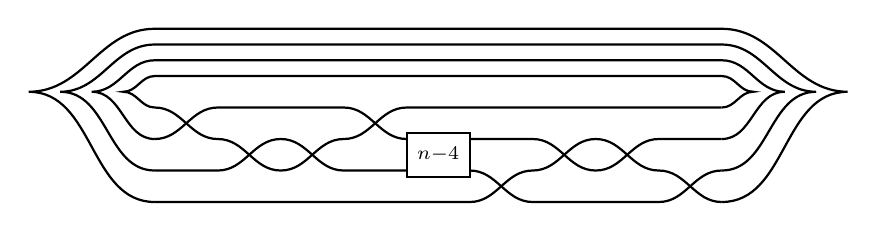
\begin{tikzpicture}[baseline=0ex,scale=0.8]
%braidpart
\draw[thick] (0,0) to[out=0,in=180] (1,-0.5) to[out=0,in=180] (2,-1) to[out=0,in=180] (3,-0.5) to[out=0,in=180] (4,0) to[out=0,in=180] (9,0);
\draw[thick] (0,-0.5) to[out=0,in=180] (1,0) to[out=0,in=180] (3,0) to[out=0,in=180] (4,-0.5) (5,-0.5) to[out=0,in=180] (6,-0.5) to[out=0,in=180] (7,-1) to[out=0,in=180] (8,-0.5) to[out=0,in=180] (9,-0.5);
\draw[thick] (0,-1) to[out=0,in=180] (1,-1) to[out=0,in=180] (2,-0.5) to[out=0,in=180] (3,-1) to[out=0,in=180] (4,-1) (5,-1) to[out=0,in=180] (6,-1.5) to[out=0,in=180] (8,-1.5) to[out=0,in=180] (9,-1);
\draw[thick] (0,-1.5) to[out=0,in=180] (5,-1.5) to[out=0,in=180] (6,-1) to[out=0,in=180] (7,-0.5) to[out=0,in=180] (8,-1) to[out=0,in=180] (9,-1.5);
\draw[thick] (4,-0.4) rectangle node {$\scriptstyle{n-4}$} (5, -1.1);
%closure part
\draw[thick] (0,0) to[out=180,in=0] (-0.5,0.25) to[out=0,in=180] (0,0.5) to[out=0,in=180] (9,0.5) to[out=0,in=180] (9.5,0.25) to[out=180,in=0] (9,0);
\draw[thick] (0,-0.5) to[out=180,in=0] (-1,0.25) to[out=0,in=180] (0,0.75) to[out=0,in=180] (9,0.75) to[out=0,in=180] (10,0.25) to[out=180,in=0] (9,-0.5);
\draw[thick] (0,-1) to[out=180,in=0] (-1.5,0.25) to[out=0,in=180] (0,1) to[out=0,in=180] (9,1) to[out=0,in=180] (10.5,0.25) to[out=180,in=0] (9,-1);
\draw[thick] (0,-1.5) to[out=180,in=0] (-2,0.25) to[out=0,in=180] (0,1.25) to[out=0,in=180] (9,1.25) to[out=0,in=180] (11,0.25) to[out=180,in=0] (9,-1.5);
\end{tikzpicture}
\end{align*}
as the rainbow closure of the positive braid $\beta_0(\exdynD_n)$
\[
\beta_0({\exdynD}_n)=\sigma_3\sigma_2\sigma_2\sigma_3 \sigma_2^{n-4} \sigma_1 \sigma_2 \sigma_2 \sigma_1.
\]

Then the Legendrian link $\legendrian({\exdynD}_n)$ admits the brick quiver diagram $\quiver^{\mathsf{brick}}({\exdynD}_n)$.

\begin{align*}
\quiver^{\mathsf{brick}}({\exdynD}_n)&=
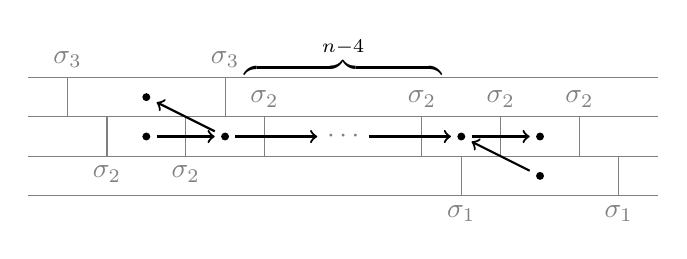
\begin{tikzpicture}[baseline=-5.5ex]
\draw[gray] (0,0) to (8,0) (0,-0.5) to (8,-0.5) (0,-1) to (8,-1) (0,-1.5) to (8,-1.5);
\draw[gray] (0.5,0) node[above] {$\sigma_3$} to (0.5,-0.5) (2.5,0) node[above] {$\sigma_3$} to (2.5,-0.5) 
(1,-0.5) to (1,-1) node[below] {$\sigma_2$} (2,-0.5) to (2,-1)node[below] {$\sigma_2$} (3,-0.5) node[above] {$\sigma_2$} to (3,-1) (5,-0.5) node[above] {$\sigma_2$} to (5,-1) (6,-0.5)  node[above] {$\sigma_2$} to (6,-1) (7,-0.5)  node[above] {$\sigma_2$} to (7,-1)
(5.5,-1) to (5.5,-1.5)node[below] {$\sigma_1$} (7.5,-1) to (7.5,-1.5) node[below] {$\sigma_1$} (4,-0.75) node (dots) {$\cdots$};
\draw[thick,fill] 
(1.5,-0.25) circle (1pt) node (D1) {}
(1.5,-0.75) circle (1pt) node (D2) {}
(2.5,-0.75) circle (1pt) node (D3) {}
(5.5,-0.75) circle (1pt) node (D4) {}
(6.5,-0.75) circle (1pt) node (D5) {}
(6.5,-1.25) circle (1pt) node (D6) {}
;
\draw (4,-0.5) node[yshift=5ex] {$\overbrace{\hphantom{\hspace{2.5cm}}}^{n-4}$};
\draw[thick,->] (D2) to (D3);
\draw[thick,->] (D3) to (dots);
\draw[thick,->] (dots) to (D4);
\draw[thick,->] (D4) to (D5);
\draw[thick,->] (D3) to (D1);
\draw[thick,->] (D6) to (D4);
\end{tikzpicture}
\end{align*}

\begin{align*}
(\ngraph^{\mathsf{brick}}(\exdynD_n),\nbasis^{\mathsf{brick}}(\exdynD_n))=
\begin{tikzpicture}[baseline=10ex, xscale=0.6, yscale=0.4]
\draw[rounded corners=5, thick] (0, 0) rectangle (14, 7);
\clip[rounded corners=5] (0, 0) rectangle (14, 7);
\draw[color=cyclecolor1, line cap=round, line width=5, opacity=0.5]
(1,5)--(4,5) (10,5)--(13,5) (2,1)--(3,1) (5,1)--(6,1) (8,1)--(9,1) (11,1)--(12,1);
\draw[color=cyan, line cap=round, line width=5, opacity=0.5]
(3,1)--(5,1) (4,1)--(4,5) (9,1)--(11,1) (10,1)--(10,5) (6,1)--(6.5,1) (7.5,1)--(8,1);
\draw[blue,thick,rounded corners]
(0,3)--(6,3)--(8,2)--(9,2)--(10,1) (10,1)--(11,2)--(12,2)--(13,1) (13,1)--(13.5,2)--(14,2)
(0,5)--(6,5)--(8,6)--(14,6)
(1,3)--(1,5) (4,3)--(4,5) (10,0)--(10,1) (13,0)--(13,1);
\draw[red,thick,rounded corners] (0,1)--(6.5,1) (7.5,1)--(14,1)
(0,4)--(0.5,4)--(1,3) (1,3)--(2,4)--(3,4)--(4,3) (4,3)--(5,4)--(9,4)--(10,3) (10,3)--(11,4)--(12,4)--(13,3) (13,3)--(13.5,4)--(14,4)
(2,0)--(2,1) (3,0)--(3,1) (5,0)--(5,1) (6,0)--(6,1) (8,0)--(8,1) (9,0)--(9,1) (11,0)--(11,1) (12,0)--(12,1)
(1,1)--(1,3) (4,1)--(4,3) (10,1)--(10,3) (13,1)--(13,3);
\draw[red,thick, dashed] (6.5,1)--(7.5,1);
\draw[green,thick,rounded corners]
(0,2)--(0.5,2)--(1,1) (1,1)--(2,2)--(3,2)--(4,1) (4,1)--(5,2)--(6,2)--(8,3)--(14,3)
(0,6)--(6,6)--(8,5)--(14,5)
(1,0)--(1,1) (4,0)--(4,1) (10,3)--(10,5) (13,3)--(13,5);
\draw[fill, blue, thick]
(1,5) circle (2pt) (4,5) circle (2pt);
\draw[fill, red, thick]
(2,1) circle (2pt) (3,1) circle (2pt) (5,1) circle (2pt) (6,1) circle (2pt) (8,1) circle (2pt) (9,1) circle (2pt)
(11,1) circle (2pt) (12,1) circle (2pt);
\draw[fill, green, thick]
(10,5) circle (2pt) (13,5) circle (2pt);
\draw[fill=white, thick]
(1,1) circle (2pt) (4,1) circle (2pt) (10,1) circle (2pt) (13,1) circle (2pt) (1,3) circle (2pt) (4,3) circle (2pt) (10,3) circle (2pt) (13,3) circle (2pt);
\end{tikzpicture}
\end{align*}

In $J^1\sphere^1$, the Legendrian link $\legendrian(\exdynD_n)$ is presented by the closure of $\beta(\exdynD_n)$
\begin{align*}
\tilde\beta(\exdynD_{n})&=\left(\sigma_2\sigma_1^3\sigma_2\sigma_1^3\sigma_2\sigma_1^k\sigma_3\right)
\cdot\left(\sigma_2\sigma_1^3\sigma_2\sigma_1^3\sigma_2\sigma_1^\ell\sigma_3\right)\\
&\mathrel{\dot{=}}\sigma_1^2\sigma_2\sigma_1^3\sigma_2\sigma_3\sigma_1^k{\color{blue}\sigma_2\sigma_1}\cdot
\sigma_1^2\sigma_2\sigma_1^3\sigma_2\sigma_3\sigma_1^\ell{\color{blue}\sigma_2\sigma_1}\\
&=\sigma_1{\color{blue}\sigma_2\sigma_1\sigma_2}\sigma_1^2\sigma_2\sigma_3{\color{blue}\sigma_2\sigma_1\sigma_2^k}\cdot
\sigma_1^2\sigma_2\sigma_1^3\sigma_2{\color{red}\sigma_1^\ell\sigma_3}\sigma_2\sigma_1\\
&=\sigma_1\sigma_2\sigma_1\sigma_2\sigma_1^2{\color{blue}\sigma_3\sigma_2\sigma_3}\sigma_1\sigma_2^k \cdot
\sigma_1^2\sigma_2\sigma_1^2{\color{red}\sigma_2^\ell\sigma_1\sigma_2}\sigma_3\sigma_2\sigma_1\\
&=\sigma_1\sigma_2\sigma_1\sigma_2{\color{blue}\sigma_3\sigma_1^2}\sigma_2{\color{blue}\sigma_1\sigma_3}\sigma_2^k \cdot
\sigma_1^2\sigma_2\sigma_1^2{\color{red}\sigma_2^\ell\sigma_1\sigma_2}\sigma_3\sigma_2\sigma_1\\
&=\sigma_1\sigma_2\sigma_1\sigma_2\sigma_3{\color{blue}\sigma_2\sigma_1\sigma_2^2}\sigma_3\sigma_2^k \cdot
\sigma_1{\color{blue}\sigma_2\sigma_1\sigma_2}\sigma_1\sigma_2^\ell\sigma_1\sigma_2\sigma_3\sigma_2\sigma_1\\
&=\sigma_1\sigma_2\sigma_1{\color{blue}\sigma_3\sigma_2\sigma_3}\sigma_1\sigma_2^2\sigma_3\sigma_2^k \cdot
\sigma_1\sigma_2\sigma_1{\color{blue}\sigma_1^\ell\sigma_2\sigma_1}\sigma_1\sigma_2\sigma_3\sigma_2\sigma_1\\
&=\sigma_1\sigma_2\sigma_1\sigma_3\sigma_2{\color{blue}\sigma_1\sigma_3}\sigma_2^2\sigma_3\sigma_2^k \cdot
{\color{blue}\sigma_2^\ell\sigma_1\sigma_2}{\color{blue}\sigma_2\sigma_1\sigma_2}\sigma_1\sigma_2\sigma_3\sigma_2\sigma_1\\
&=\Delta_4\beta_0(\exdynD_{n})\Delta_4,
\end{align*}
where $k=\lfloor \frac{n-3}2\rfloor$ and $\ell=\lfloor \frac{n-4}2\rfloor$.

\begin{definition}[$N$-graph of type $\exdynD_{n}$]
We define a free $4$-graph $\ngraph(\exdynD_{n})$ for $\legendrian(\exdynD_n)$ as depicted in the left of Figure~\ref{figure:4-graph of type affine Dn}.
\end{definition}

\begin{figure}[ht]
\subfigure[$\ngraph(\exdynD_{2n}), n\ge 2$]
{
\begin{tikzpicture}[baseline=-.5ex,scale=0.6]
\draw[rounded corners=5, thick] (-6.5, -2.5) rectangle (6.5, 2.5);
\draw (0.5, -2.5) node[above] {$\cdots$} 
(-0.5, -2.5) node[below] {$\underbrace{\hphantom{\hspace{3cm}}}_{n-2}$};
\draw (1.5, 2.5) node[below] {$\cdots$} 
(0.5, 2.5) node[above] {$\overbrace{\hphantom{\hspace{3cm}}}^{n-2}$};
\clip[rounded corners=5] (-6.5, -2.5) rectangle (6.5, 2.5);
\draw[cyclecolor1, opacity=0.5, line cap=round, line width=5] 
(-3.5, 0) -- (-2.5, 0) (-3.5, 0) -- (-4.5, 1) (-3.5, 0) -- (-4.5, -1)
(-1.5, 0) -- (-0.5, 0)
(0.5, 0) -- (1.5, 0)
(3.5, 0) -- (2.5, 0) (3.5, 0) -- (4.5, 1) (3.5, 0) -- (4.5, -1)
;
\draw[cyclecolor2, opacity=0.5, line cap=round, line width=5] 
(-4.5, 1) -- (-5.5, 1)
(-4.5, -1) -- (-4.5, -1.75)
(-1.5, 0) -- (-2.5, 0)
(-0.5, 0) -- (0.5, 0)
(1.5, 0) -- (2.5, 0)
(4.5, 1) -- (4.5, 1.75)
(4.5, -1) -- (5.5, -1)
;
\foreach \i in {0, 180} {
\begin{scope}[rotate=\i]
\draw[thick, green] (-2.5, 2.5) -- (0,0);
\draw[thick, red] 
(-3.5, -2.5) -- (-3.5, 2.5)
(-6.5, 0) -- (-3.5, 0)
;
\draw[thick, blue, fill]
(-2.5, -2.5) -- (-2.5,0) circle (2pt)
(-0.5, -2.5) -- (-0.5,0) circle (2pt)
(1.5, -2.5) -- (1.5,0) circle (2pt)
;
\draw[thick, blue, fill] 
%
(-3.5, 0) -- (3.5, 0)
(-3.5, 0) -- (-4.5, 1) circle (2pt) -- (-4.5, 2.5)
(-4.5, 1) -- (-6.5, 1)
(-5.5, 1) circle (2pt) -- (-5.5, 2.5)
%
(-3.5, 0) -- (-4.5, -1) circle (2pt) -- (-4.5, -2.5)
(-4.5, -1) -- (-6.5, -1)
(-4.5, -1.73) circle (2pt) -- (-6.5, -1.73)
;
\end{scope}
}
\draw[thick, fill=white] (-3.5, 0) circle (2pt) (3.5, 0) circle (2pt);
\end{tikzpicture}
}

\subfigure[$\ngraph(\exdynD_{2n+1}), n\ge 2$]
{
\begin{tikzpicture}[baseline=-.5ex,scale=0.6]
\draw[rounded corners=5, thick] (-6, -2.5) rectangle (6, 2.5);
\draw (-1, -2.5) node[above] {$\cdots$} (1, -2.5) node[above] {$\cdots$}
(0, -2.5) node[below] {$\underbrace{\hphantom{\hspace{3cm}}}_{n-1}$};
\draw (0, 2.5) node[below] {$\cdots$} 
(0, 2.5) node[above] {$\overbrace{\hphantom{\hspace{1.5cm}}}^{n-2}$};
\draw[cyclecolor1, opacity=0.5, line cap=round, line width=5] 
(-3, 0) -- (-2, 0) (-3, 0) -- (-4, 1) (-3, 0) -- (-4, -1)
(-1, 0) -- (-0, 0)
(1, 0) -- (2, 0)
(4, -1) -- (4, -1.75)
(4, 1) -- (5, 1)
;
\draw[cyclecolor2, opacity=0.5, line cap=round, line width=5] 
(0, 0) -- (1, 0)
(3, 0) -- (2, 0) (3, 0) -- (4, 1) (3, 0) -- (4, -1)
(-4, 1) -- (-5, 1)
(-4, -1) -- (-4, -1.75)
(-1, 0) -- (-2, 0)
;
\clip[rounded corners=5] (-6.5, -2.5) rectangle (6.5, 2.5);
\draw[thick, green] (-2.5, 2.5) -- (2.5,-2.5);
\foreach \i in {1, -1} {
\begin{scope}[xshift=\i*0.5cm, xscale=\i]
\draw[thick, red] 
(-3.5, -2.5) -- (-3.5, 2.5)
(-6.5, 0) -- (-3.5, 0)
;
\draw[thick, blue, fill]
(-2.5, -2.5) -- (-2.5,0) circle (2pt)
(-1.5, 2.5) -- (-1.5,0) circle (2pt)
(-0.5, -2.5) -- (-0.5,0) circle (2pt)
;
\draw[thick, blue, fill] 
%
(-3.5, 0) -- (0, 0)
(-3.5, 0) -- (-4.5, 1) circle (2pt) -- (-4.5, 2.5)
(-4.5, 1) -- (-6.5, 1)
(-5.5, 1) circle (2pt) -- (-5.5, 2.5)
%
(-3.5, 0) -- (-4.5, -1) circle (2pt) -- (-4.5, -2.5)
(-4.5, -1) -- (-6.5, -1)
(-4.5, -1.73) circle (2pt) -- (-6.5, -1.73)
;
\draw[thick, fill=white] (-3.5, 0) circle (2pt);
\end{scope}
}
\end{tikzpicture}
}

\caption{$N$-graph of type $\exdynD_n$}
\label{figure:4-graph of type affine Dn}
\end{figure}

\begin{lemma}\label{lemma:Ngraphs of affine Dn}
The $N$-graphs $\ngraph(\exdynD_n)$ and $\ngraph^{\mathsf{brick}}(\exdynD_n)$ are equivalent up to $\boundary$-Legendrian isotopy and Legendrian mutations.
\end{lemma}
The pictorial proof of the lemma will be given in Appendix~\ref{appendix:Ngraph of type affine Dn}.

As before, the freeness is obvious since $\ngraph(\exdynD_n)$ consists of trees.
Moreover, $\ngraph(\exdynD_{2n})$ has a $\pi$-rotation symmetry. That is, we obtain the following lemma.
\begin{lemma}
The pair $\ngraph(\exdynD_{2n})$ is invariant under $\pi$-rotation.
\end{lemma}



\subsubsection{The degenerate $4$-graph of type $\exdynD_4$}
The final $N$-graph we introduce is a degenerate $4$-graph $\tilde\ngraph(\exdynD_4)$ of type $\exdynD_4$ as follows:
\[
\tilde\ngraph(\exdynD_4)=
\begin{tikzpicture}[baseline=-.5ex, scale=0.8]
\draw (0,0) circle (3);
\clip (0,0) circle (3);
\foreach \r in {0, 180} {
\begin{scope}[rotate=\r]
\draw[fill, red, thick]
(3,-3) -- (-3,3) 
(0,0) -- (45:2) circle (2pt)
(45:2) -- ++(0,3)
(45:2) -- ++(3,0)
(45:2) ++ (0.75,0) circle (2pt) -- ++(0,2)
;
\draw[Dble={blue and green},line width=2] (0,0) -- (0,3);
\draw[Dble={green and blue},line width=2] (0,0) -- (2,0);
\draw[Dble={green and blue},line width=2] (2,0) -- ++(-45:2);
\draw[Dble={green and blue},line width=2] (2,0) -- ++(45:2);
\end{scope}
}
\end{tikzpicture}
\]
which defines a bipartite quiver of type $\exdynD_4$.

The boundary Legendrian link $\tilde\legendrian(\exdynD_4)$ is the closure of 
\begin{align*}
\tilde\beta(\exdynD_4)&=\sigma_2\sigma_{1,3}\sigma_2\sigma_{1,3}^2\sigma_2^3\sigma_{1,3}\sigma_2\sigma_{1,3}^2\sigma_2^2\\
&=\Delta_4 \sigma_{1,3} \sigma_2^2 \Delta_4 \sigma_{1,3}\sigma_2^2\\
&=\sigma_3\Delta_4 \sigma_3 \sigma_2^2 \sigma_{1,3}\sigma_2^2 \Delta_4\\
&\mathrel{\dot{=}}\Delta_4 \sigma_3\sigma_2^2 \sigma_3 \sigma_1 \sigma_2^2\Delta_4 \sigma_3\\
&=\Delta_4 \beta_0(\exdynD_4) \Delta_4.
\end{align*}

\begin{lemma}
The $4$-graph $\tilde\ngraph(\exdynD_4)$ is equivalent to the $4$-graph $\ngraph(\exdynD_4)$ up to $\boundary$-Legendrian isotopy and Legendrian mutations.
\end{lemma}
See Appendix~\ref{appendix:affine D4} for the proof.



\subsubsection{Exchange graphs corresponding to linear or tripod \texorpdfstring{$N$-graphs}{N-graphs}}
Notice that the $N$-graphs $\ngraph(\dynX)$ and $\ngraph^{\mathsf{brick}}(\dynX)$ are deterministic for $\dynX = \dynA,\dynD,\dynE,\exdynD, \exdynE$.
Therefore, the coefficients in $\bfy(\ngraph(\dynX),\nbasis(\dynX))$ are defined on $\bbC[\cM(\legendrian(\dynX))]$. Here, $\cM(\legendrian)$ is the moduli spaces of flags on $\legendrian$ and is turned out to be a cluster Poisson variety as seen in Remark~\ref{remark:Poisson variety}. 

On the other hand, one can show that the variables $\{X_a\}_{a\in I_\legendrian}$, Shen--Weng constructed in~\cite[\S 3.2]{SW2019}, coincide with the coefficients in the coefficient tuple $\bfy(\ngraph^{\mathsf{brick}}(a,b,c),\nbasis^{\mathsf{brick}}(a,b,c))$ or $\bfy(\ngraph^{\mathsf{brick}}(n),\nbasis^{\mathsf{brick}}(n))$. Moreover, coefficients are algebraically independent.
In summary, we have the following corollary, which is a direct consequence of the above discussion, Proposition~\ref{prop_Y-pattern_exchange_graph}, and~\eqref{eq_exchange_graphs_are_the_same}.
\begin{corollary}\label{corollary:algebraic independence}
Let $(\ngraph_{t_0},\nbasis_{t_0})$ be either $(\ngraph(a,b,c), \nbasis(a,b,c))$ or $(\ngraph(n), \nbasis(n))$ of type $\dynX$, and let $(\bfy_{t_0},\qbasispr_{t_0})=\Psi(\ngraph_{t_0}, \nbasis_{t_0})$ and $\qbasispr_{t_0}=\qbasispr(\quiver(\ngraph_{t_0},\nbasis_{t_0}))$.
Then the exchange graph of the $Y$-pattern given by the initial $Y$-seed $(\bfy_{t_0},\qbasispr_{t_0})$ is the same as the exchange graph $\exchange(\Roots)$ of the root system~$\Roots$ of type $\dynX$.
\end{corollary}


\subsection{Legendrian Coxeter mutations}

For a bipartite quiver $\quiver$, we have two sets of vertices $I_+$ and
$I_-$ so that all edges are oriented from $I_+$ to $I_-$.
Let $\mutation_+$ and $\mutation_-$ be sequences of mutations defined by 
compositions of mutations corresponding to each and every vertex in $I_+$ and 
$I_-$, respectively.
A Coxeter mutation~$\qcoxeter$ and its inverse $\qcoxeter^{-1}$ are the compositions
\begin{align*}
\mutation_\quiver&=\prod_{i\in I_+}\mutation_i \cdot \prod_{i\in I_-} \mutation_i,&
\mutation_\quiver^{-1}&=\prod_{i\in I_-}\mutation_i \cdot \prod_{i\in I_+} \mutation_i.
\end{align*}
Note that $\prod_{i\in I_+}\mutation_i$ does not depend on the order of composition of mutations $\mutation_i$ among $i\in I_+$, and the same holds for $I_-$.

\begin{remark}\label{rmk_mutation_convention}
For any sequence $\mutation$ of mutations, we will use the right-to-left convention. Namely, the rightmost mutation will be applied first on the quiver $\quiver$.
\end{remark}

Similarly, we define the Legendrian Coxeter mutation, which will be denoted by $\ncoxeter$, on a bipartite $N$-graph $\ngraph$ as follows:
\begin{definition}[Legendrian Coxeter mutation]
For a bipartite $N$-graph $\ngraph$ with decomposed sets of cycles $\nbasis=\nbasis_+\cup\nbasis_-$, we define the \emph{Legendrian Coxeter mutation} $\ncoxeter$ and its inverse $\ncoxeter^{-1}$ as the compositions of Legendrian mutations
\begin{align*}
\mu_\ngraph&=\prod_{\gamma\in \nbasis_+}\mutation_\gamma \cdot \prod_{\gamma\in \nbasis_-}\mutation_\gamma,&
\mu_\ngraph^{-1}&=\prod_{\gamma\in \nbasis_-}\mutation_\gamma \cdot \prod_{\gamma\in \nbasis_+}\mutation_\gamma.
\end{align*}
\end{definition}

It is worth mentioning that each $\mutation_\ngraph^{\pm1}$ does not depend on the order of mutations if cycles in each of $\nbasis_\pm$ are disjoint. 
This directly implies that $\mutation_\ngraph^{-1}$ is indeed the inverse of 
$\mutation_\ngraph$. Note that all cycles in each of $\nbasis_\pm(\dynX)$ for $\dynX =\dynA,\dynD,\dynE,\exdynD, \exdynE$ are disjoint as seen in Figures~\ref{figure:linear N-graph}, \ref{figure:tripod N-graph}, and \ref{figure:4-graph of type affine Dn}.


\subsubsection{Legendrian Coxeter mutation for linear $N$-graphs}

\begin{lemma}\label{lemma:Legendriam Coxeter mutation of type An}
The effect of the Legendrian Coxeter mutation on $(\ngraph(\dynA_n),\nbasis(\dynA_n))$ is the clockwise $\frac{2\pi}{n+3}$-rotation and therefore
\[
\ncoxeter(\ngraph(\dynA_n),\nbasis(\dynA_n))=
\coxeterpadding(\dynA_n)(\ngraph(\dynA_n),\nbasis(\dynA_n)),
\]
where $\coxeterpadding(\dynA_n)$ is an annular $N$-graph called the \emph{Coxeter padding} of type $\dynA_n$ as follows:
\begin{equation}\label{equation:Coxeter padding of type An}
\coxeterpadding(\dynA_n)=
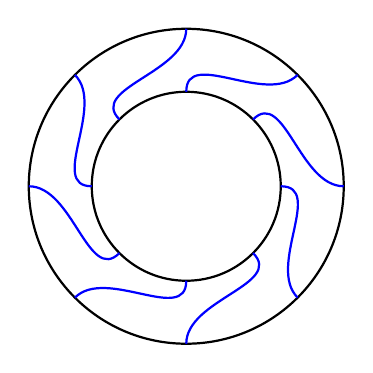
\begin{tikzpicture}[baseline=-.5ex,scale=0.4]
\draw[thick] (0,0) circle (5) (0,0) circle (3);
\foreach \i in {45, 90, ..., 360} {
\draw[blue, thick] (\i:5) to[out=\i-180,in=\i+45] (\i+45:3);
}
\end{tikzpicture}
\end{equation}
\end{lemma}
\begin{proof}
We may assume that the Coxeter element $\ncoxeter$ can be represented by the sequence
\[
\ncoxeter=\mutation_+\mutation_-=(\mutation_{\cycle_2}\mutation_{\cycle_4}\mutation_{\cycle_6}\cdots)(\mutation_{\cycle_1}\mutation_{\cycle_3}\mutation_{\cycle_5}\dots).
\]
Then the action of $\ncoxeter$ on $\ngraph(\dynA_n)$ is as depicted in Figure~\ref{figure:Legendrian Coxeter mutation on An}, which is nothing but the clockwise $\frac{2\pi}{n+3}$-rotation of the original $N$-graph $(\ngraph(\dynA_n),\nbasis(\dynA_n))$ as claimed.

The last statement is obvious as seen in Figure~\ref{figure:coxeter padding of type An}.
\end{proof}

\begin{figure}[ht]
\subfigure[Legendrian Coxeter mutation for $\ngraph(\dynA_n)$\label{figure:Legendrian Coxeter mutation on An}]{
\begin{tikzcd}[ampersand replacement=\&]
\begin{tikzpicture}[baseline=-.5ex,xscale=0.6,yscale=0.6]
\draw[thick] (0,0) circle (3);
\draw[color=cyclecolor2, line cap=round, line width=5, opacity=0.5] (-1.5,0.5) -- (-0.5, -0.5) (0.5, 0.5) -- (1.5, -0.5);
\draw[color=cyclecolor1, line cap=round, line width=5, opacity=0.5] (-2.5,-0.5) -- (-1.5, 0.5) (-0.5, -0.5) -- (0.5, 0.5) (1.5, -0.5) -- (2.5, 0.5);
\draw[blue, thick, fill] (0:3) -- (2.5,0.5) circle (2pt) -- (45:3) (2.5,0.5) -- (1.5,-0.5) circle (2pt) -- (-45:3) (1.5,-0.5) -- (0.5,0.5) circle (2pt) -- (90:3)
(0.5, 0.5) -- (-0.5, -0.5) circle (2pt) -- (-90:3) (-0.5, -0.5) -- (-1.5, 0.5) circle (2pt) -- (135:3) (-1.5, 0.5) -- (-2.5, -0.5) circle (2pt) -- (-135:3);
\draw[blue, thick] (-2.5,-0.5) -- (-180:3);
\draw (0,-3) node[below] {$(\ngraph(\dynA_n),\nbasis(\dynA_n))$};
\end{tikzpicture}
\arrow[r,|->,"\mutation_-"] \&
\begin{tikzpicture}[baseline=-.5ex, xscale=0.6,yscale=0.6]
\begin{scope}[yscale=-1]
\draw[thick] (0,0) circle (3);
\draw[color=cyclecolor2, line cap=round, line width=5, opacity=0.5] (-1.5,0.5) -- (-0.5, -0.5) (0.5, 0.5) -- (1.5, -0.5);
\draw[color=cyclecolor1, line cap=round, line width=5, opacity=0.5] (-2.5,-0.5) -- (-1.5, 0.5) (-0.5, -0.5) -- (0.5, 0.5) (1.5, -0.5) -- (2.5, 0.5);
\draw[blue, thick, fill] (0:3) -- (2.5,0.5) circle (2pt) -- (45:3) (2.5,0.5) -- (1.5,-0.5) circle (2pt) -- (-45:3) (1.5,-0.5) -- (0.5,0.5) circle (2pt) -- (90:3)
(0.5, 0.5) -- (-0.5, -0.5) circle (2pt) -- (-90:3) (-0.5, -0.5) -- (-1.5, 0.5) circle (2pt) -- (135:3) (-1.5, 0.5) -- (-2.5, -0.5) circle (2pt) -- (-135:3);
\draw[blue, thick] (-2.5,-0.5) -- (-180:3);
\end{scope}
\draw (0,-3) node[below] {$(\ngraph(\dynA_n),\nbasis(\dynA_n))$};
\end{tikzpicture}
\arrow[r,|->,"\mutation_+"] \&
\begin{tikzpicture}[baseline=-.5ex, xscale=0.6,yscale=0.6]
\begin{scope}[rotate=-45]
\draw[thick] (0,0) circle (3);
\draw[color=cyclecolor2, line cap=round, line width=5, opacity=0.5] (-1.5,0.5) -- (-0.5, -0.5) (0.5, 0.5) -- (1.5, -0.5);
\draw[color=cyclecolor1, line cap=round, line width=5, opacity=0.5] (-2.5,-0.5) -- (-1.5, 0.5) (-0.5, -0.5) -- (0.5, 0.5) (1.5, -0.5) -- (2.5, 0.5);
\draw[blue, thick, fill] (0:3) -- (2.5,0.5) circle (2pt) -- (45:3) (2.5,0.5) -- (1.5,-0.5) circle (2pt) -- (-45:3) (1.5,-0.5) -- (0.5,0.5) circle (2pt) -- (90:3)
(0.5, 0.5) -- (-0.5, -0.5) circle (2pt) -- (-90:3) (-0.5, -0.5) -- (-1.5, 0.5) circle (2pt) -- (135:3) (-1.5, 0.5) -- (-2.5, -0.5) circle (2pt) -- (-135:3);
\draw[blue, thick] (-2.5,-0.5) -- (-180:3);
\end{scope}
\draw (0,-3) node[below] {$\mutation_\ngraph(\ngraph(\dynA_n),\nbasis(\dynA_n))$};
\end{tikzpicture}
\end{tikzcd}
}

\subfigure[Coxeter padding $\coxeterpadding(\dynA_n)$ of type $\dynA_n$\label{figure:coxeter padding of type An}]{$
\begin{tikzpicture}[baseline=-.5ex, xscale=0.6,yscale=0.6]
\begin{scope}[rotate=-45]
\draw[thick] (0,0) circle (3);
\draw[color=cyclecolor2, line cap=round, line width=5, opacity=0.5] (-1.5,0.5) -- (-0.5, -0.5) (0.5, 0.5) -- (1.5, -0.5);
\draw[color=cyclecolor1, line cap=round, line width=5, opacity=0.5] (-2.5,-0.5) -- (-1.5, 0.5) (-0.5, -0.5) -- (0.5, 0.5) (1.5, -0.5) -- (2.5, 0.5);
\draw[blue, thick, fill] (0:3) -- (2.5,0.5) circle (2pt) -- (45:3) (2.5,0.5) -- (1.5,-0.5) circle (2pt) -- (-45:3) (1.5,-0.5) -- (0.5,0.5) circle (2pt) -- (90:3)
(0.5, 0.5) -- (-0.5, -0.5) circle (2pt) -- (-90:3) (-0.5, -0.5) -- (-1.5, 0.5) circle (2pt) -- (135:3) (-1.5, 0.5) -- (-2.5, -0.5) circle (2pt) -- (-135:3);
\draw[blue, thick] (-2.5,-0.5) -- (-180:3);
\end{scope}
\draw (0,-3) node[below] {$\mutation_\ngraph(\ngraph(\dynA_n),\nbasis(\dynA_n))$};
\end{tikzpicture}
=
\begin{tikzpicture}[baseline=-.5ex,xscale=0.6,yscale=0.6]
\draw[thick] (0,0) circle (5);
\foreach \i in {45, 90, ..., 360} {
\draw[blue, thick] (\i:5) to[out=\i-180,in=\i+45] (\i+45:3);
}
%
\draw[thick] (0,0) circle (3);
\draw[color=cyclecolor2, line cap=round, line width=5, opacity=0.5] (-1.5,0.5) -- (-0.5, -0.5) (0.5, 0.5) -- (1.5, -0.5);
\draw[color=cyclecolor1, line cap=round, line width=5, opacity=0.5] (-2.5,-0.5) -- (-1.5, 0.5) (-0.5, -0.5) -- (0.5, 0.5) (1.5, -0.5) -- (2.5, 0.5);
\draw[blue, thick, fill] (0:3) -- (2.5,0.5) circle (2pt) -- (45:3) (2.5,0.5) -- (1.5,-0.5) circle (2pt) -- (-45:3) (1.5,-0.5) -- (0.5,0.5) circle (2pt) -- (90:3)
(0.5, 0.5) -- (-0.5, -0.5) circle (2pt) -- (-90:3) (-0.5, -0.5) -- (-1.5, 0.5) circle (2pt) -- (135:3) (-1.5, 0.5) -- (-2.5, -0.5) circle (2pt) -- (-135:3);
\draw[blue, thick] (-2.5,-0.5) -- (-180:3);
\draw (0,-5) node[below] {$\coxeterpadding(\dynA_n)(\ngraph(\dynA_n),\nbasis(\dynA_n))$};
\end{tikzpicture}
$}
\caption{Legendrian Coxeter mutation $\ncoxeter$ on $(\ngraph(\dynA_n), \nbasis(\dynA_n))$}
\end{figure}

\begin{remark}\label{rmk_order_of_Coxeter_mutation}
The order of the Coxeter mutation is either $(n+3)/2$ if $n$ is odd or $n+3$ otherwise.
Since the Coxeter number $h=n+1$ for $\dynA_n$, this verifies Lemma~\ref{lemma:order of coxeter mutation} in this case.
\end{remark}

\subsubsection{Legendrian Coxeter mutation for tripod $N$-graphs}

Let us consider the Legendrian Coxeter mutation for tripod $N$-graphs.
By the mutation convention mentioned in Remark~\ref{rmk_mutation_convention}, for each tripod $\ngraph(a,b,c)$, we always take a mutation at the central $\sfY$-cycle $\cycle$ first.
After the Legendrian mutation on $(\ngraph(a,b,c),\nbasis(a,b,c))$ at $\cycle$, we have the $N$-graph on the left in Figure~\ref{figure:center mutation}.
Then there are three shaded regions that we can apply the generalized push-through moves so that we obtain the $N$-graph on the right in Figure~\ref{figure:center mutation}.
\begin{figure}[ht]
\subfigure[\label{figure:center mutation}After the mutation at the central vertex]{
\begin{tikzcd}[ampersand replacement=\&]
\begin{tikzpicture}[baseline=-.5ex,xscale=0.8, yscale=0.8]
\begin{scope}
\fill[opacity=0.1](85:3) to[out=-90,in=150] (60:1.3) arc (60:-60:0.3) arc (120:240:0.7) to[out=-30,in=150] (-25:3) arc (-25:85:3);
\end{scope}
\begin{scope}[rotate=120]
\fill[opacity=0.1](85:3) to[out=-90,in=150] (60:1.3) arc (60:-60:0.3) arc (120:240:0.7) to[out=-30,in=150] (-25:3) arc (-25:85:3);
\end{scope}
\begin{scope}[rotate=240]
\fill[opacity=0.1](85:3) to[out=-90,in=150] (60:1.3) arc (60:-60:0.3) arc (120:240:0.7) to[out=-30,in=150] (-25:3) arc (-25:85:3);
\end{scope}
\draw[thick] (0,0) circle (3cm);
\draw[color=cyclecolor2, line cap=round, line width=5, opacity=0.5] (50:1.5) to[out=-60,in=60] (0:1) -- (-60:1) (70:1.75) -- (50:2) (170:1.5) to[out=60,in=180] (120:1) -- (60:1) (190:1.75) -- (170:2) (290:1.5) to[out=180,in=300] (240:1) -- (180:1) (310:1.75) -- (290:2);
\draw[color=cyclecolor1, line cap=round, line width=5, opacity=0.5] (0,0) -- (60:1) (0,0) -- (180:1) (0,0) -- (300:1) (50:1.5) -- (70:1.75) (170:1.5) -- (190:1.75) (290:1.5) -- (310:1.75);
\draw[blue, thick] (0,0) -- (0:1) (0,0) -- (120:1) (0,0) -- (240:1);
\draw[red, thick, fill] (0,0) -- (60:1) circle (2pt) (0,0) -- (180:1) circle (2pt) (0,0) -- (300:1) circle (2pt);
\draw[red, thick] (0:1) -- (0:3) (120:1) -- (120:3) (240:1) -- (240:3);
\draw[red, thick] (60:1) -- (120:1) -- (180:1) -- (240:1) -- (300:1) -- (0:1) -- cycle;
\draw[blue, thick] (100:3) to[out=-80,in=60] (120:1) (-20:3) to[out=-200,in=-60] (0:1) (220:3) to[out=40,in=180] (240:1);
\draw[blue, thick] (50:1.5) to[out=-60,in=60] (0:1) (170:1.5) to[out=60,in=180] (120:1) (290:1.5) to[out=180,in=300] (240:1);
\draw[blue, thick, fill] (50:1.5) circle (2pt) -- (20:3) (50:1.5) -- (70:1.75) circle (2pt) -- (80:3) (70:1.75) -- (50:2) circle (2pt) -- (40:3);
\draw[blue, thick, dashed] (50:2) -- (60:3);
\draw[blue, thick, fill] (170:1.5) circle (2pt) -- (140:3) (170:1.5) -- (190:1.75) circle (2pt) -- (200:3) (190:1.75) -- (170:2) circle (2pt) -- (160:3);
\draw[blue, thick, dashed] (170:2) -- (180:3);
\draw[blue, thick, fill] (290:1.5) circle (2pt) -- (260:3) (290:1.5) -- (310:1.75) circle (2pt) -- (320:3) (310:1.75) -- (290:2) circle (2pt) -- (280:3);
\draw[blue, thick, dashed] (290:2) -- (300:3);
\draw[thick,fill=white] (0:1) circle (2pt) (120:1) circle (2pt) (240:1) circle (2pt);
\draw[thick, fill=white] (0,0) circle (2pt);
\end{tikzpicture}\arrow[r,"\Move{II^*}"]\&
\begin{tikzpicture}[baseline=-.5ex,xscale=0.6, yscale=0.6]
\draw[thick] (0,0) circle (5cm);
\draw[dashed]  (0,0) circle (3cm);
\fill[opacity=0.1, even odd rule] (0,0) circle (3) (0,0) circle (5);
\foreach \i in {1,2,3} {
\begin{scope}[rotate=\i*120]
\begin{scope}[shift=(60:0.5)]
\fill[opacity=0.1, rounded corners] (0,0) -- (0:2) arc (0:120:2) -- cycle;
\end{scope}
\draw[color=cyclecolor2, line cap=round, line width=5, opacity=0.5] (60:1) -- (70:1.5) (90:1.75) -- (70:2);
\draw[color=cyclecolor1, line cap=round, line width=5, opacity=0.5] (0,0) -- (60:1) (70:1.5) -- (90:1.75);
%
\draw[blue, thick, rounded corners] (0,0) -- (0:3.4) to[out=-75,in=80] (-40:4);
\draw[red, thick, fill] (0,0) -- (60:1) circle (2pt) (60:1) -- (70:1.5) circle (2pt) -- (90:1.75) circle (2pt) -- (70:2) circle (2pt);
\draw[red, thick, dashed, rounded corners] (70:2) -- (60:2.8) -- (60:3.3) to[out=0,in=220] (40:4) (40:4) to[out=120,in=-20] (60:4);
\draw[red, thick, rounded corners] (70:1.5) -- (40:2.8) -- (40:3.3) to[out=-20,in=200] (20:4) (70:2) -- (80:2.8) -- (80:3.3) to[out=20,in=240] (60:4) (90:1.75) -- (100:2.8) -- (100:3.3) to[out=40,in=260] (80:4);
\draw[red, thick, rounded corners] (60:1) -- (20:3) -- (20:3.5) to[out=-70,in=50] (-40:4) (20:4) to[out=-50,in=120] (0:4.5) -- (0:5);
\draw[red, thick] (20:4) to[out=100,in=-40] (40:4) (60:4) to[out=140,in=0] (80:4);
\draw[blue, thick] (20:5) -- (20:4) to[out=140,in=-80] (40:4) (60:5) -- (60:4) to[out=180,in=-40] (80:4) -- (80:5);
\draw[blue, thick, rounded corners] (20:4) to[out=-70,in=100] (-20:4.5) -- (-20:5);
\draw[blue, thick, dashed] (40:4) to[out=160,in=-60] (60:4) (40:4) -- (40:5);
\draw[fill=white, thick] (20:4) circle (2pt) (40:4) circle (2pt) (60:4) circle (2pt) (80:4) circle (2pt) (-40:4) circle (2pt);
\end{scope}
\draw[fill=white, thick] (0,0) circle (2pt);
}
\end{tikzpicture}
\end{tikzcd}}
\subfigure[\label{figure:coxeter mutation}After Legendrian Coxeter mutation]{$
%t\cdot \ngraph(a,b,c)=
\begin{tikzpicture}[baseline=-.5ex,xscale=0.6, yscale=0.6]
\draw[thick] (0,0) circle (5cm);
\draw[dashed]  (0,0) circle (3cm);
\fill[opacity=0.1, even odd rule] (0,0) circle (3) (0,0) circle (5);
\foreach \i in {1,2,3} {
\begin{scope}[rotate=\i*120]
\draw[color=cyclecolor2, line cap=round, line width=5, opacity=0.5] (60:1) -- (50:1.5) (70:1.75) -- (50:2);
\draw[color=cyclecolor1, line cap=round, line width=5, opacity=0.5] (0,0) -- (60:1) (50:1.5) -- (70:1.75);
%
\draw[blue, thick, rounded corners] (0,0) -- (0:3.4) to[out=-75,in=80] (-40:4);
\draw[red, thick, fill] (0,0) -- (60:1) circle (2pt) (60:1) -- (50:1.5) circle (2pt) -- (70:1.75) circle (2pt) -- (50:2) circle (2pt);
\draw[red, thick, dashed, rounded corners] (50:2) -- (60:2.8) -- (60:3.3) to[out=0,in=220] (40:4) (40:4) to[out=120,in=-20] (60:4);
\draw[red, thick, rounded corners] (50:2) -- (40:2.8) -- (40:3.3) to[out=-20,in=200] (20:4) (70:1.75) -- (80:2.8) -- (80:3.3) to[out=20,in=240] (60:4) (60:1) -- (100:2.8) -- (100:3.3) to[out=40,in=260] (80:4);
\draw[red, thick, rounded corners] (50:1.5) -- (20:3) -- (20:3.5) to[out=-70,in=50] (-40:4) (20:4) to[out=-50,in=120] (0:4.5) -- (0:5);
\draw[red, thick] (20:4) to[out=100,in=-40] (40:4) (60:4) to[out=140,in=0] (80:4);
\draw[blue, thick] (20:5) -- (20:4) to[out=140,in=-80] (40:4) (60:5) -- (60:4) to[out=180,in=-40] (80:4) -- (80:5);
\draw[blue, thick, rounded corners] (20:4) to[out=-70,in=100] (-20:4.5) -- (-20:5);
\draw[blue, thick, dashed] (40:4) to[out=160,in=-60] (60:4) (40:4) -- (40:5);
\draw[fill=white, thick] (20:4) circle (2pt) (40:4) circle (2pt) (60:4) circle (2pt) (80:4) circle (2pt) (-40:4) circle (2pt);
\end{scope}
\draw[fill=white, thick] (0,0) circle (2pt);
}
\end{tikzpicture}
$}
\caption{Legendrian Coxeter mutation for $(\ngraph(a,b,c),\nbasis(a,b,c))$} 
\end{figure}
Notice that in each triangular shaded region, the $N$-subgraph looks like the $N$-graph of type $\dynA_{a-1}, \dynA_{b-1}$, or $\dynA_{c-1}$.
Moreover, the mutations corresponding to the rest sequence is just a composition 
of Legendrian Coxeter mutations of type $\dynA_{a-1},\dynA_{b-1}$, and $\dynA_{c-1}$, 
which are essentially the same as the clockwise rotations by Lemma~\ref{lemma:Legendriam Coxeter mutation of type An}.
Therefore, the result of the Legendrian Coxeter mutation will be given as depicted in 
Figure~\ref{figure:coxeter mutation}.

Then the resulting $N$-graph becomes very similar to the original $N$-graph $\ngraph(a,b,c)$.
Indeed, the inside is identical to $\ngraph(a,b,c)$ but the colors are switched, which is the conjugation $\overline{\ngraph(a,b,c)}$ by definition.
The complement of $\overline{\ngraph(a,b,c)}$ in $\qcoxeter(\ngraph(a,b,c),\nbasis(a,b,c))$ is an annular $N$-graph.

\begin{definition}[Coxeter padding of type $(a,b,c)$]
For each triple $a,b,c$, the annular $N$-graph depicted in Figure~\ref{figure:coxeter padding} is denoted by $\coxeterpadding(a,b,c)$ and called the \emph{Coxeter padding} of type $(a,b,c)$.
We also denote the Coxeter padding with color switched by $\overline{\coxeterpadding(a,b,c)}$, which is the conjugation of $\coxeterpadding(a,b,c)$.
\end{definition}

\begin{figure}[ht]
\subfigure[$\coxeterpadding(a,b,c)$]{\makebox[0.48\textwidth]{
$
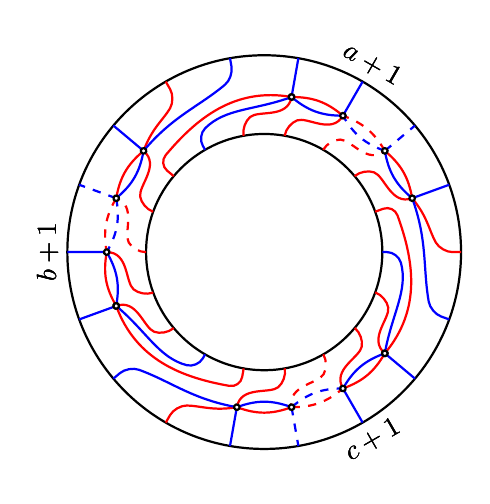
\begin{tikzpicture}[baseline=-.5ex,scale=0.5]
\draw[thick] (0,0) circle (5) (0,0) circle (3);
\foreach \i in {1,2,3} {
\begin{scope}[rotate=\i*120]
\draw[blue, thick, rounded corners] (0:3) -- (0:3.4) to[out=-75,in=80] (-40:4);
\draw[red, thick, dashed, rounded corners] (60:3) -- (60:3.3) to[out=0,in=220] (40:4) (40:4) to[out=120,in=-20] (60:4);
\draw[red, thick, rounded corners] (40:3) -- (40:3.3) to[out=-20,in=200] (20:4) (80:3) -- (80:3.3) to[out=20,in=240] (60:4) (100:3) -- (100:3.3) to[out=40,in=260] (80:4);
\draw[red, thick, rounded corners] (20:3) -- (20:3.5) to[out=-70,in=50] (-40:4) (20:4) to[out=-50,in=120] (0:4.5) -- (0:5);
\draw[red, thick] (20:4) to[out=100,in=-40] (40:4) (60:4) to[out=140,in=0] (80:4);
\draw[blue, thick] (20:5) -- (20:4) to[out=140,in=-80] (40:4) (60:5) -- (60:4) to[out=180,in=-40] (80:4) -- (80:5);
\draw[blue, thick, rounded corners] (20:4) to[out=-70,in=100] (-20:4.5) -- (-20:5);
\draw[blue, thick, dashed] (40:4) -- (40:5) (40:4) to[out=160,in=-60] (60:4);
\draw[fill=white, thick] (20:4) circle (2pt) (40:4) circle (2pt) (60:4) circle (2pt) (80:4) circle (2pt) (-40:4) circle (2pt);
\end{scope}
\curlybrace[]{10}{110}{5.2};
\draw (60:5.5) node[rotate=-30] {$a+1$};
\curlybrace[]{130}{230}{5.2};
\draw (180:5.5) node[rotate=90] {$b+1$};
\curlybrace[]{250}{350}{5.2};
\draw (300:5.5) node[rotate=30] {$c+1$};
}
\end{tikzpicture}$
}}
\subfigure[$\overline{\coxeterpadding(a,b,c)}$]{\makebox[0.48\textwidth]{
$
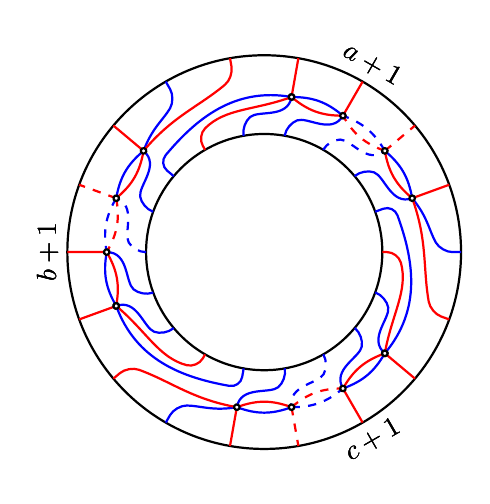
\begin{tikzpicture}[baseline=-.5ex,scale=0.5]
\draw[thick] (0,0) circle (5) (0,0) circle (3);
\foreach \i in {1,2,3} {
\begin{scope}[rotate=\i*120]
\draw[red, thick, rounded corners] (0:3) -- (0:3.4) to[out=-75,in=80] (-40:4);
\draw[blue, thick, dashed, rounded corners] (60:3) -- (60:3.3) to[out=0,in=220] (40:4) (40:4) to[out=120,in=-20] (60:4);
\draw[blue, thick, rounded corners] (40:3) -- (40:3.3) to[out=-20,in=200] (20:4) (80:3) -- (80:3.3) to[out=20,in=240] (60:4) (100:3) -- (100:3.3) to[out=40,in=260] (80:4);
\draw[blue, thick, rounded corners] (20:3) -- (20:3.5) to[out=-70,in=50] (-40:4) (20:4) to[out=-50,in=120] (0:4.5) -- (0:5);
\draw[blue, thick] (20:4) to[out=100,in=-40] (40:4) (60:4) to[out=140,in=0] (80:4);
\draw[red, thick] (20:5) -- (20:4) to[out=140,in=-80] (40:4) (60:5) -- (60:4) to[out=180,in=-40] (80:4) -- (80:5);
\draw[red, thick, rounded corners] (20:4) to[out=-70,in=100] (-20:4.5) -- (-20:5);
\draw[red, thick, dashed] (40:4) -- (40:5) (40:4) to[out=160,in=-60] (60:4);
\draw[fill=white, thick] (20:4) circle (2pt) (40:4) circle (2pt) (60:4) circle (2pt) (80:4) circle (2pt) (-40:4) circle (2pt);
\end{scope}

\curlybrace[]{10}{110}{5.2};
\draw (60:5.5) node[rotate=-30] {$a+1$};
\curlybrace[]{130}{230}{5.2};
\draw (180:5.5) node[rotate=90] {$b+1$};
\curlybrace[]{250}{350}{5.2};
\draw (300:5.5) node[rotate=30] {$c+1$};
}
\end{tikzpicture}$
}}
\\
\subfigure[$\coxeterpadding(a,b,c)^{-1}$]{\makebox[0.48\textwidth]{
$
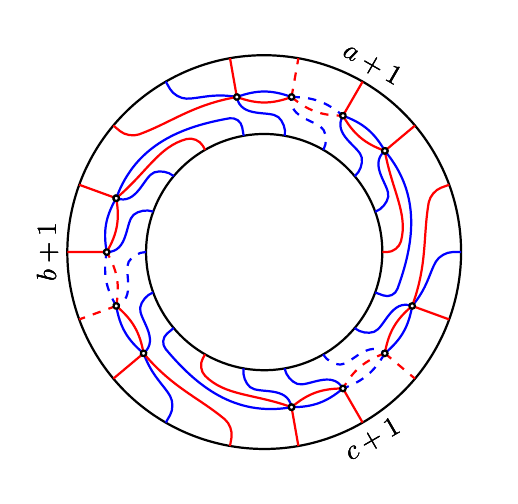
\begin{tikzpicture}[baseline=-.5ex,xscale=-0.5,yscale=0.5,rotate=60]
\draw[thick] (0,0) circle (5) (0,0) circle (3);
\foreach \i in {1,2,3} {
\begin{scope}[rotate=\i*120]
\draw[red, thick, rounded corners] (0:3) -- (0:3.4) to[out=-75,in=80] (-40:4);
\draw[blue, thick, dashed, rounded corners] (60:3) -- (60:3.3) to[out=0,in=220] (40:4) (40:4) to[out=120,in=-20] (60:4);
\draw[blue, thick, rounded corners] (40:3) -- (40:3.3) to[out=-20,in=200] (20:4) (80:3) -- (80:3.3) to[out=20,in=240] (60:4) (100:3) -- (100:3.3) to[out=40,in=260] (80:4);
\draw[blue, thick, rounded corners] (20:3) -- (20:3.5) to[out=-70,in=50] (-40:4) (20:4) to[out=-50,in=120] (0:4.5) -- (0:5);
\draw[blue, thick] (20:4) to[out=100,in=-40] (40:4) (60:4) to[out=140,in=0] (80:4);
\draw[red, thick] (20:5) -- (20:4) to[out=140,in=-80] (40:4) (60:5) -- (60:4) to[out=180,in=-40] (80:4) -- (80:5);
\draw[red, thick, rounded corners] (20:4) to[out=-70,in=100] (-20:4.5) -- (-20:5);
\draw[red, thick, dashed] (40:4) -- (40:5) (40:4) to[out=160,in=-60] (60:4);
\draw[fill=white, thick] (20:4) circle (2pt) (40:4) circle (2pt) (60:4) circle (2pt) (80:4) circle (2pt) (-40:4) circle (2pt);
\end{scope}

\curlybrace[]{10}{110}{5.2};
\draw (60:5.5) node[rotate=-30] {$a+1$};
\curlybrace[]{130}{230}{5.2};
\draw (180:5.5) node[rotate=30] {$c+1$};
\curlybrace[]{250}{350}{5.2};
\draw (300:5.5) node[rotate=90] {$b+1$};
}
\end{tikzpicture}$
}}
\subfigure[$\overline{\coxeterpadding(a,b,c)}^{-1}$]{\makebox[0.48\textwidth]{
$
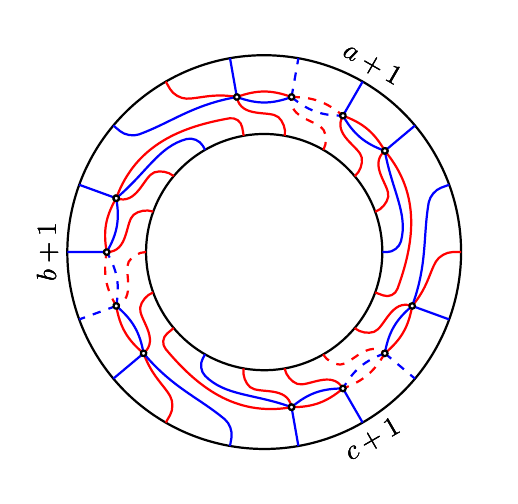
\begin{tikzpicture}[baseline=-.5ex,xscale=-0.5, yscale=0.5,rotate=60]
\draw[thick] (0,0) circle (5) (0,0) circle (3);
\foreach \i in {1,2,3} {
\begin{scope}[rotate=\i*120]
\draw[blue, thick, rounded corners] (0:3) -- (0:3.4) to[out=-75,in=80] (-40:4);
\draw[red, thick, dashed, rounded corners] (60:3) -- (60:3.3) to[out=0,in=220] (40:4) (40:4) to[out=120,in=-20] (60:4);
\draw[red, thick, rounded corners] (40:3) -- (40:3.3) to[out=-20,in=200] (20:4) (80:3) -- (80:3.3) to[out=20,in=240] (60:4) (100:3) -- (100:3.3) to[out=40,in=260] (80:4);
\draw[red, thick, rounded corners] (20:3) -- (20:3.5) to[out=-70,in=50] (-40:4) (20:4) to[out=-50,in=120] (0:4.5) -- (0:5);
\draw[red, thick] (20:4) to[out=100,in=-40] (40:4) (60:4) to[out=140,in=0] (80:4);
\draw[blue, thick] (20:5) -- (20:4) to[out=140,in=-80] (40:4) (60:5) -- (60:4) to[out=180,in=-40] (80:4) -- (80:5);
\draw[blue, thick, rounded corners] (20:4) to[out=-70,in=100] (-20:4.5) -- (-20:5);
\draw[blue, thick, dashed] (40:4) -- (40:5) (40:4) to[out=160,in=-60] (60:4);
\draw[fill=white, thick] (20:4) circle (2pt) (40:4) circle (2pt) (60:4) circle (2pt) (80:4) circle (2pt) (-40:4) circle (2pt);
\end{scope}
\curlybrace[]{10}{110}{5.2};
\draw (60:5.5) node[rotate=-30] {$a+1$};
\curlybrace[]{130}{230}{5.2};
\draw (180:5.5) node[rotate=30] {$c+1$};
\curlybrace[]{250}{350}{5.2};
\draw (300:5.5) node[rotate=90] {$b+1$};
}
\end{tikzpicture}$
}}
\caption{Coxeter paddings $\coxeterpadding(a,b,c)$, $\bar\coxeterpadding(a,b,c)$ and their inverses.}
\label{figure:coxeter padding}
\end{figure}

Notice that two Coxeter paddings $\coxeterpadding(a,b,c)$ and $\overline{\coxeterpadding(a,b,c)}$ can be glued without any ambiguity
and so we can also pile up Coxeter paddings $\coxeterpadding(a,b,c)$ and $\overline{\coxeterpadding(a,b,c)}$ alternatively as many times as we want.

We also define the concatenation of the Coxeter padding $\overline{\coxeterpadding(a,b,c)}$ on the pair $(\ngraph(a,b,c),\nbasis(a,b,c))$ as the pair $(\ngraph', \nbasis')$ such that
\begin{enumerate}
\item the $N$-graph $\ngraph'$ is obtained by gluing $\overline{\coxeterpadding(a,b,c)}$ on $\ngraph(a,b,c)$, and 
\item the set $\nbasis'$ of cycles is the set of $\sfI$- and $\sfY$-cycles identified with $\nbasis(a,b,c)$ in a canonical way.
\end{enumerate}

\begin{proposition}\label{proposition:effect of Legendrian Coxeter mutation}
Let $(\ngraph, \nbasis) = (\ngraph(a,b,c), \nbasis(a,b,c))$.
The Legendrian Coxeter mutation on $(\ngraph, \nbasis)$ or $\overline{(\ngraph,\nbasis)}$ is given as the concatenation
\begin{align*}
\ncoxeter(\ngraph, \nbasis) &= \coxeterpadding\overline{(\ngraph,\nbasis)},&
\ncoxeter^{-1}(\ngraph, \nbasis) &= \bar\coxeterpadding^{-1}\overline{(\ngraph,\nbasis)},&
\ncoxeter\overline{(\ngraph,\nbasis)} &= \bar \coxeterpadding (\ngraph, \nbasis),&
\ncoxeter^{-1}\overline{(\ngraph,\nbasis)} &= \coxeterpadding^{-1} (\ngraph, \nbasis),
\end{align*}
where $\coxeterpadding=\coxeterpadding(a,b,c)$, $\bar\coxeterpadding=\overline{\coxeterpadding(a,b,c)}$.

In general, for $r\ge 0$, we have
\begin{align*}
\ncoxeter^r(\ngraph,\nbasis) &= \begin{cases}
\coxeterpadding\bar\coxeterpadding\cdots \bar\coxeterpadding (\ngraph,\nbasis)& \text{ if }r\text{ is even},\\
\coxeterpadding\bar\coxeterpadding\cdots \coxeterpadding \overline{(\ngraph,\nbasis)}& \text{ if }r\text{ is odd}.
\end{cases}\\
\ncoxeter^{-r}(\ngraph,\nbasis) &= \begin{cases}
\bar\coxeterpadding^{-1}\coxeterpadding^{-1}\cdots \coxeterpadding^{-1} (\ngraph,\nbasis)& \text{ if }r\text{ is even},\\
\bar\coxeterpadding^{-1}\coxeterpadding^{-1}\cdots \bar\coxeterpadding^{-1} \overline{(\ngraph,\nbasis)}& \text{ if }r\text{ is odd}.
\end{cases}
\end{align*}
\end{proposition}
\begin{proof}
This follows directly from the above observation.
\end{proof}

It is important that this proposition holds only when we take the Legendrian Coxeter mutation on the very standard $N$-graph $\ngraph(a,b,c)$ with the cycles $\nbasis(a,b,c)$.
Otherwise, the Legendrian Coxeter mutation will not be expressed as simple as above.


Let $(\ngraph, \nbasis)$ be a pair of a deterministic $N$-graph, a set of good cycles.
Suppose that the quiver~$\quiver(\ngraph,\nbasis)$ is bipartite and the Legendrian Coxeter mutation $\ncoxeter(\ngraph,\nbasis)$ is realizable.
Then, by Proposition~\ref{proposition:equivariance of mutations}, we have
\[
\Psi(\ncoxeter(\ngraph,\nbasis)) = \qcoxeter(\Psi(\ngraph,\nbasis)).
\]
In particular, for quivers of type $\dynA_n$ or tripods, we have the following corollary.
\begin{corollary}\label{corollary:Coxeter mutations}
For each $n\ge 1$ and $a,b,c\ge 1$, the Legendrian Coxeter mutation $\ncoxeter$ on $(\ngraph(\dynA_n),\nbasis(\dynA_n))$ or $(\ngraph(a,b,c),\nbasis(a,b,c))$ corresponds to the Coxeter mutation $\qcoxeter$ on $\quiver(\dynA_n)$ or $\quiver(a,b,c)$, respectively.
In other words,
\begin{align*}
\Psi(\ncoxeter(\ngraph(\dynA_n),\nbasis(\dynA_n))) &= \qcoxeter(\Psi(\ngraph(\dynA_n),\nbasis(\dynA_n)));\\
\Psi(\ncoxeter(\ngraph(a,b,c),\nbasis(a,b,c))) &= \qcoxeter(\Psi(\ngraph(a,b,c),\nbasis(a,b,c))).
\end{align*}
\end{corollary}


\begin{theorem}\label{theorem:infinite fillings}
For $a,b,c\ge 1$ with $\frac 1a+\frac1b+\frac1c\le 1$,
The Legendrian knot or link $\legendrian(a,b,c)$ in $J^1\sphere^1$ admits infinitely many distinct exact embedded Lagrangian fillings.
\end{theorem}
\begin{proof}
By Proposition~\ref{proposition:effect of Legendrian Coxeter mutation}, the effect of the Legendrian Coxeter mutation on $(\ngraph(a,b,c), \nbasis(a,b,c))$ is just to attach the Coxeter padding on $(\bar\ngraph(a,b,c),\bar\nbasis(a,b,c))$.
In particular, as mentioned earlier, the iterated Legendrian Coxeter mutation
\[
\ncoxeter^r(\ngraph(a,b,c), \nbasis(a,b,c))
\]
is well-defined for each $r\in\mathbb{Z}$.
Each of these $N$-graphs defines a Legendrian weave $\Legendrian(\ncoxeter^r(\ngraph(a,b,c), \nbasis(a,b,c)))$, whose Lagrangian projection is a Lagrangian filling 
\[
L_r(a,b,c)\colonequals(\pi\circ\iota)(\Legendrian(\ncoxeter^r(\ngraph(a,b,c), \nbasis(a,b,c)))
\]
as desired. Therefore it suffices to prove that Lagrangians $L_r(a,b,c)$ for $r\ge 0$ are pairwise distinct up to exact Lagrangian isotopy when $\frac1a+\frac1b+\frac1c\le 1$.

Now suppose that $\frac1a+\frac1b+\frac1c\le1$, or equivalently, $\quiver(a,b,c)$ is of infinite type, that is, it is not of finite Dynkin type (cf. Definition~\ref{def_quiver_of_type_X}(1)).
Then the order of the Coxeter mutation is infinite by Lemma~\ref{lemma:order of coxeter mutation} and so is the order of the Legendrian Coxeter mutation by Corollary~\ref{corollary:Coxeter mutations}.
In particular, the set 
\[
\left\{\Psi(\ncoxeter^r(\ngraph(a,b,c), \nbasis(a,b,c)))\mid r\in\mathbb{Z}\right\}
\]
is a set of infinitely many pairwise distinct $Y$-seeds in the $Y$-pattern for $\quiver(a,b,c)$.
Hence, by Corollary~\ref{corollary:distinct seeds imples distinct fillings}, we have pairwise distinct Lagrangian fillings $L_r(a,b,c)$.
\end{proof}

\begin{remark}
For Legendrian links of non $\dynADE$-type, there are lots of examples having infinitely many distinct Lagrangian fillings given by a number of different researchers and groups. A non-exhaustive list includes \cite{CG2020, CN2021, CZ2020, GSW2020b}.
\end{remark}


\subsubsection{Legendrian Coxeter mutations for $N$-graphs of type $\exdynD_n$}
We will perform the Legendrian Coxeter mutation $\mutation_\ngraph$ on $(\ngraph(\exdynD_n), \nbasis(\exdynD_n))$ in order to provide the pictorial proof of Proposition~\ref{proposition:coxeter realization D-type}.

Before we take mutations, we first introduce a useful operation on $N$-graphs 
described below, called the \emph{move} $\mathrm{(Z)}$.
\[
\begin{tikzcd}
\begin{tikzpicture}[baseline=-.5ex,scale=0.5]
\draw[cyclecolor2, line cap=round, line width=5, opacity=0.5] (-2,1)--(-1,1) (-1,-1)--(-1,-2);
\draw[cyclecolor1, line cap=round, line width=5, opacity=0.5,] (-1,1)--(0,0) (-1,-1)--(0,0) (0,0)--(1,0);
\draw[red, thick] (0,3) -- (0,-3) (0,0) -- (-3,0);
\draw[blue,thick, fill] (0,0) -- (-1,1) circle (2pt) -- +(0,2) (-1,1) -- ++(-1,0) circle (2pt) -- +(-1,0) (-2,1) -- +(0,2);
\draw[blue,thick, fill] (0,0) -- (-1,-1) circle (2pt) -- +(-2,0) (-1,-1) -- ++(0,-1) circle (2pt) -- +(0,-1) (-1,-2) -- +(-2,0);
\draw[blue,thick] (0,0) -- (1,0);
\draw[thick, fill=white] (0,0) circle (2pt);
\end{tikzpicture}\arrow[r,"\mathrm{(II)}"]&
\begin{tikzpicture}[baseline=-.5ex,scale=0.5]
\draw[cyclecolor2, line cap=round, line width=5, opacity=0.5] (-2,1)--(-1,1) (-1,-2)--(1,0)--(1,1);
\draw[cyclecolor1, line cap=round, line width=5, opacity=0.5] (-1,1)--(0,0) (0,0)--(2,0);
\draw[red, thick, fill] (1,3) -- (1,1) circle (2pt) -- (0,0) (1,1) -- (1,0) (1,0) -- (1,-3) (1,0) -- (-3,0);
\node at (-0.5,0.5)[above right] {$\gamma$};
\draw[blue, thick] (0,0) to[out=30,in=150] (1,0);
\draw[blue,thick, fill] (0,0) -- (-1,1) circle (2pt) -- +(0,2) (-1,1) -- ++(-1,0) circle (2pt) -- +(-1,0) (-2,1) -- +(0,2) (-1,-2) circle (2pt);
\draw[blue,thick]  (-1,-3) -- (-1,-2) -- (1,0) (-1,-2) -- (-3,-2);
\draw[blue,thick,rounded corners](0,0) -- (-1,-1) -- +(-2,0);
\draw[blue,thick] (1,0) -- (2,0);
\draw[thick, fill=white] (0,0) circle (2pt) (1,0) circle (2pt);
\end{tikzpicture}\arrow[r,"\mu_\gamma"]&
\begin{tikzpicture}[baseline=-.5ex,scale=0.5]
\draw[cyclecolor2, line cap=round, line width=5, opacity=0.5] (-2,2)--(-1,1) (0,-2)--(1,-1)--(1,0) to[out=120,in=-120] (1,1) -- (1,2);
\draw[cyclecolor1, line cap=round, line width=5, opacity=0.5,] (-1,1)--(0,1)--(1,0)--(2,0);
\draw[red, thick, fill] (1,3) -- (1,-3) (-3,0) -- (-1,0) (1,2) circle (2pt) -- (0,2);
\draw[red, thick] (1,1) -- (0,2) -- (0,1) -- (1,0) (0,1) -- (-1,0) -- (1,-1);
\draw[blue, thick, fill] (0,2) -- (-1,3) (0,1) -- (-1,1) circle (2pt) -- (-2,2) circle (2pt) -- (-2,3) (-1,1) -- (-1,0) (-2,2) -- (-3,2) (1,-1) -- (0,-2) circle (2pt) -- (-3,-2) (0,-2) -- (0,-3);
\draw[blue,thick, rounded corners] (-1,0) -- (-2,-1) -- (-3,-1) ;
\draw[blue, thick] (1,1) -- (2,1) (1,0) -- (2,0) (1,-1) -- (2,-1);
\draw[blue, thick] (-1,0) to[out=15,in=-105] (0,1) (0,2) to[out=-15,in=105] (1,1) (1,1) to[out=-120,in=120] (1,0) (1,0) to[out=-120,in=120] (1,-1) (0,2) to[out=-60,in=60] (0,1);
\draw[thick, fill=white] (-1,0) circle (2pt) (1,0) circle (2pt) (0,1) circle (2pt) (0,2) circle (2pt) (1,1) circle (2pt) (1,-1) circle (2pt);
\end{tikzpicture}\arrow[r,"\mathrm{(II)}"]&
\begin{tikzpicture}[baseline=-.5ex,scale=0.5]
\draw[cyclecolor2, line cap=round, line width=5, opacity=0.5] (-2,2)--(-1,1) (0,-2)--(1,-1)--(1,0)--(0.67, 0.67);
\draw[cyclecolor1, line cap=round, line width=5, opacity=0.5,] (-1,1)--(0,1)--(1,0)--(2,0);
\draw[red, thick, fill] (1,3)--(1,-3) (-3,0) -- (-1,0) (-1,0) -- (1,-1) (1,1) -- (0,1);
\draw[red, thick] (-1,0) -- (0,1) -- (1,0);
\draw[blue, thick, fill] (1,1) -- (0.67, 0.67) circle (2pt) -- (0,1) (0.67, 0.67) -- (1,0);
\draw[blue, thick] (-1,0) to[out=15, in=-105] (0,1) (1,0) to[out=-120,in=120] (1,-1);
\draw[blue, thick, fill] (0,1) -- (-1,1) circle (2pt) -- (-2,2) circle (2pt) -- (-2,3) (-1,0) -- (-1,1) (-2,2) -- (-3,2);
\draw[blue, thick] (1,1) -- (0,2) -- (-1,3);
\draw[blue, thick] (1,1) -- ++(1,0) (1,0) -- ++(1,0) (1,-1) -- ++(1,0);
\draw[blue, thick, fill] (1,-1) -- (0,-2) circle (2pt) -- (-3,-2) (0,-2) -- (0,-3) ;
\draw[blue,thick, rounded corners] (-1,0) -- (-2,-1) -- (-3,-1) ;
\draw[thick, fill=white] (-1,0) circle (2pt) (0,1) circle (2pt) (1,-1) circle (2pt) (1,0) circle (2pt) (1,1) circle (2pt);
\end{tikzpicture}\arrow[d, "\mathrm{(II)}"]\\
\begin{tikzpicture}[baseline=-.5ex,scale=0.5]
\draw[cyclecolor2, line cap=round, line width=5, opacity=0.5, line cap=round] 
(1,0.5) -- (1,1.5)
(0.5,-1) --(1.5,-1)
;
\draw[cyclecolor1, line cap=round, line width=5, opacity=0.5] 
(1,0.5) -- (2,0) --(1.5,-1)
(2,0) -- (3,0)
;
\draw[red, thick] 
(2,3) -- (2,-3)
(2,2) -- (0,2) -- (-2,0) -- (-3,0)
(2,-2) -- (0,-2) -- (-2,0)
(0,2) -- (0,-2)
(0,0) -- (2,0)
;
\draw[blue, thick] 
(-3,1) -- (-2,0) to[out=15,in=-105] (0,2) -- (-1,3)
(0,2) -- (1,1.5) -- (2,2) -- (3,2)
(1,3) -- (2,2)
(1,1.5) -- (1,0.5) -- (2,0) -- (3,0)
(1,0.5) -- (0,0) -- (0.5,-1) -- (1.5,-1) -- (2,0)
(0,0) to[out=-120,in=120] (0,-2) -- (-1,-3)
(0,-2) -- (0.5,-1)
(1.5,-1) -- (2,-2) -- (3,-2)
(2,-2) -- (1,-3)
(-3,-1) -- (-2,0)
;
\draw[thick, fill=white] 
(-2,0) circle (2pt) 
(0,2) circle (2pt) 
(0,-2) circle (2pt) 
(0,0) circle (2pt) 
(2,2) circle (2pt) 
(2,0) circle (2pt) 
(2,-2) circle (2pt);
\draw[blue, thick, fill]
(1,0.5) circle (2pt)
(1,1.5) circle (2pt)
(0.5,-1) circle (2pt)
(1.5,-1) circle (2pt)
; 
\end{tikzpicture}
&
\begin{tikzpicture}[baseline=-.5ex,scale=0.5]
\draw[cyclecolor2, line cap=round, line width=5, opacity=0.5] 
(-2,2)--(-1,2)--(-1,0)--(0,-1) 
(0,0.5)--(0,1.5);
\draw[cyclecolor1, line cap=round, line width=5, opacity=0.5,] (0,-1)--(1,0)--(2,0) (0,0.5)--(1,0);
\draw[red, thick] (1,3)--(1,-3) (-3,0) -- (-1,2)--(1,2) (-1,2) --(-1,0)--(1,0) (-1,0) to[out=-90,in=180] (1,-2);
\draw[blue, thick] 
(-3,2) -- (-2,2) -- (-2,3) 
(-2,2) -- (-1,2) -- (0,1.5) -- (1,2) -- (0,3)
(2,2)--(1,2) 
(0,1.5)--(0,0.5)--(1,0)--(2,0) 
(0,0.5)--(-1,0) -- (-2,-3)
(0,-3) --(1,-2) -- (2,-2)
(1,-2) -- (-1,0)
(0,-1) -- (1,0)
(-1,2) -- (-3,-2)
;
\draw[blue, thick, fill] 
(-2,2) circle (2pt)
(0,1.5) circle (2pt)
(0,0.5) circle (2pt)
(0,-1) circle (2pt)
;
\draw[thick, fill=white] 
(-1,2) circle (2pt) 
(-1,0) circle (2pt) 
(1,2) circle (2pt) 
(1,0) circle (2pt) 
(1,-2) circle (2pt) 
;
\end{tikzpicture}\arrow[l,"\mathrm{(II)^2}"]
&
\begin{tikzpicture}[baseline=-.5ex,scale=0.5]
\draw[cyclecolor2, line cap=round, line width=5, opacity=0.5] (-2,2)--(-1,1) (0.5, 0.75) -- (0.5,0.25);
\draw[cyclecolor1, line cap=round, line width=5, opacity=0.5,] (-1,1)--(0,1)--(0,0) to[out=-30,in=-120] (1,0) --(2,0) (1,0) -- (0.5,0.25);
\draw[red, thick, fill] (1,3)--(1,-3) (-3,0) -- (-1,0) (-1,0) -- (0,-1) (1,1) -- (0,1) (0,0) -- (0,-1);
\draw[red, thick] (-1,0) -- (0,1) -- (0,0) -- (1,0) (0,-1) -- (1,-1);
\draw[blue, thick, fill] (1,1) -- (0.5, 0.75) circle (2pt) -- (0.5,0.25) circle (2pt) -- (1,0) (0.5, 0.75) -- (0,1) (0.5, 0.25) -- (0,0);
\draw[blue, thick] (-1,0) to[out=15, in=-105] (0,1) (0,0) to[out=-120,in=120] (0,-1) (0,-1) to[out=30, in=150] (1,-1) (0,0) to[out=-30, in=-150] (1,0);
\draw[blue, thick, fill] (0,1) -- (-1,1) circle (2pt) -- (-2,2) circle (2pt) -- (-2,3) (-1,0) -- (-1,1) (-2,2) -- (-3,2);
\draw[blue, thick] (1,1) -- (0,2) -- (-1,3);
\draw[blue, thick] (1,1) -- ++(1,0) (1,0) -- ++(1,0) (1,-1) -- ++(1,0);
\draw[blue, thick] (0,-1) -- (-2,-3) (1,-1) -- (-1,-3) (-1,0) -- (-3,-2);
\draw[thick, fill=white] (-1,0) circle (2pt) (0,-1) circle (2pt) (0,0) circle (2pt) (0,1) circle (2pt) (1,-1) circle (2pt) (1,0) circle (2pt) (1,1) circle (2pt);
\end{tikzpicture}\arrow[l,"\mathrm{(I,II)^*}"]&
\begin{tikzpicture}[baseline=-.5ex,scale=0.5]
\draw[cyclecolor2, line cap=round, line width=5, opacity=0.5] (-2,2)--(-1,1) (1,-0.5)--(1,0)--(0.67, 0.67);
\draw[cyclecolor1, line cap=round, line width=5, opacity=0.5,] (-1,1)--(0,1)--(1,0)--(2,0);
\draw[red, thick, fill] (1,3)--(1,-3) (-3,0) -- (-1,0) (-1,0) -- (0,-1) (1,1) -- (0,1) (1,-0.5) circle (2pt) -- (0,-1);
\draw[red, thick] (-1,0) -- (0,1) -- (1,0) (0,-1) -- (1,-1);
\draw[blue, thick, fill] (1,1) -- (0.67, 0.67) circle (2pt) -- (0,1) (0.67, 0.67) -- (1,0) (1,0) -- (0,-1);
\draw[blue, thick] (-1,0) to[out=15, in=-105] (0,1) (0,-1) to[out=20, in=160] (1,-1);
\draw[blue, thick, fill] (0,1) -- (-1,1) circle (2pt) -- (-2,2) circle (2pt) -- (-2,3) (-1,0) -- (-1,1) (-2,2) -- (-3,2);
\draw[blue, thick] (1,1) -- (0,2) -- (-1,3);
\draw[blue, thick] (1,1) -- ++(1,0) (1,0) -- ++(1,0) (1,-1) -- ++(1,0);
\draw[blue, thick] (0,-1) -- (-2,-3) (1,-1) -- (-1,-3) (-1,0) -- (-3,-2);
\draw[thick, fill=white] (-1,0) circle (2pt) (0,-1) circle (2pt) (0,1) circle (2pt) (1,-1) circle (2pt) (1,0) circle (2pt) (1,1) circle (2pt);
\end{tikzpicture}\arrow[l,"\mathrm{(II)}"]
\end{tikzcd}
\]

\begin{remark}
The reader should not confuse that even though we call this operation the 
\emph{move}, it does not induce any equivalence on $N$-graphs since it involves 
a mutation $\mutation_\cycle$.
\end{remark}

One important observation is that one can take the move $\mathrm{(Z)}$ instead of the Legendrian mutation~$\mutation_\cycle$ on the $\sfY$-like cycle\footnote{We use an ambiguous terminology `$\sfY$-like cycle' since the global shape of $\cycle$ is unknown.
	However, the meaning is obvious and we omit the detail.
}~$\cycle$, and after the move, the $\sfY$-like cycle becomes the $\sfY$-like cycle and $\sfI$-cycles become $\sfI$-cycles again.

For example, let us consider $(\ngraph(\exdynD_4), \nbasis(\exdynD_4))$. Then the Legendrian Coxeter mutation $\ncoxeter(\ngraph(\exdynD_4), \nbasis(\exdynD_4))$ is obtained by the composition $(\mutation_{\cycle_2}\mutation_{\cycle_3}\mutation_{\cycle_4}\mutation_{\cycle_5})$ followed by the mutation $\mutation_{\cycle_1}$. See Figure~\ref{figure:Legendrian Coxeter mutation for affine D4}.

\begin{figure}[ht]
\[
\begin{tikzcd}
\begin{tikzpicture}[baseline=-.5ex,scale=0.4]
\draw[rounded corners=5, thick] (-4, -2.5) rectangle (4, 2.5);
\clip[rounded corners=5] (-4, -2.5) rectangle (4, 2.5);
\draw[cyclecolor1, opacity=0.5, line cap=round, line width=5]
(-1, 0) -- (1, 0) node[near start, above, color=black, sloped,opacity=1] {$\cycle_1$} (-1, 0) -- (-2, 1) (-1, 0) -- (-2, -1)
(1, 0) -- (2, 1) (1, 0) -- (2, -1)
;
\draw[cyclecolor2, opacity=0.5, line cap=round, line width=5] 
(-2, 1) -- (-3, 1) node[midway, below, color=black,opacity=1] {$\cycle_2$}
(-2, -1) -- (-2, -1.75) node[midway, right=-1ex, color=black,opacity=1] {$\cycle_3$}
(2, 1) -- (2, 1.75) node[midway, left=-1ex, color=black,opacity=1] {$\cycle_4$}
(2, -1) -- (3, -1) node[midway, above, color=black,opacity=1] {$\cycle_5$}
;
\foreach \i in {0, 180} {
\begin{scope}[rotate=\i]
\begin{scope}[xshift=2.5cm]
\draw[thick, green] (-2.5, 2.5) -- ++(0,-2.5);
\draw[thick, red] 
(-3.5, -2.5) -- (-3.5, 2.5)
(-6.5, 0) -- (-3.5, 0)
;
\draw[thick, blue, fill] 
%
(-3.5, 0) -- (-2.5, 0)
(-3.5, 0) -- (-4.5, 1) circle (2pt) -- (-4.5, 2.5)
(-4.5, 1) -- (-6.5, 1)
(-5.5, 1) circle (2pt) -- (-5.5, 2.5)
%
(-3.5, 0) -- (-4.5, -1) circle (2pt) -- (-4.5, -2.5)
(-4.5, -1) -- (-6.5, -1)
(-4.5, -1.73) circle (2pt) -- (-6.5, -1.73)
;
\end{scope}
\end{scope}
}
\draw[thick, fill=white] (-1, 0) circle (2pt) (1, 0) circle (2pt);
\end{tikzpicture}
\arrow[r,"\mutation_{\cycle_1}"]
\arrow[rd, "\ncoxeter"', bend right]
& 
\begin{tikzpicture}[baseline=-.5ex,scale=0.4]
\draw[rounded corners=5, thick] (-8, -4) rectangle (8, 4);
\clip[rounded corners=5] (-8, -4) rectangle (8, 4);
\foreach \r in {0, 180} {
\begin{scope}[rotate=\r]
\draw[blue, thick]
(-4, 1) -- ++(-1, -1)
(-4, -1) -- ++(-1, 1) to[out=-120, in=120] ++(0,-3)
(-5, 3) to[out=-105,in=30] (-7,0)
%
(-2, -2.5) -- ++(1, -0.5) -- +(-1, -1)
++(0,0) -- ++(2, 0) -- ++(1, 0.5)
(-3, -2.5) -- ++(-2, -0.5) -- ++(-1, -1)
(-4, 1.75) -- ++(-1, 1.25) -- ++(-1, 1)
(-2, 2.5) -- ++(1, 0.5) -- ++(-1, 1)
(-8, 1) -- ++(1, -1) -- ++(-1, -1)
;
\draw[red, thick] 
(-1, -2.5) -- ++(0, -0.5) -- +(0, -1)
++(0,0) -- ++(-4, 0) -- ++(0, 3) -- +(1,0)
++(0,0) -- ++(0,3) -- ++(4,0) -- +(0, 1)
++(0,0) -- ++(0, -0.5)
(-5, -3) -- ++(-2, 3) -- +(-1, 0)
++(0,0) -- ++(2, 3)
;
\draw[green, thick] (0, 4) -- (0, 2.5);
\draw[fill=white, thick] 
(-5, 0) circle (2pt) (-7, 0) circle (2pt)
(-5, -3) circle (2pt) (-1, -3) circle (2pt) (1, -3) circle (2pt)
(-5, 3) circle (2pt)
;
\end{scope}
}
\begin{scope}[yscale=-1]
\draw[rounded corners=5, thick] (-4, -2.5) rectangle (4, 2.5);
\clip[rounded corners=5] (-4, -2.5) rectangle (4, 2.5);
\draw[cyclecolor1, opacity=0.5, line cap=round, line width=5]
(-1, 0) -- (1, 0) (-1, 0) -- (-2, 1) (-1, 0) -- (-2, -1)
(1, 0) -- (2, 1) (1, 0) -- (2, -1)
;
\draw[cyclecolor2, opacity=0.5, line cap=round, line width=5] 
(-2, 1) -- (-3, 1)
(-2, -1) -- (-2, -1.75)
(2, 1) -- (2, 1.75)
(2, -1) -- (3, -1)
;
\foreach \i in {0, 180} {
\begin{scope}[rotate=\i]
\begin{scope}[xshift=2.5cm]
\draw[thick, green] (-2.5, 2.5) -- ++(0,-2.5);
\draw[thick, red] 
(-3.5, -2.5) -- (-3.5, 2.5)
(-6.5, 0) -- (-3.5, 0)
;
\draw[thick, blue, fill] 
%
(-3.5, 0) -- (-2.5, 0)
(-3.5, 0) -- (-4.5, 1) circle (2pt) -- (-4.5, 2.5)
(-4.5, 1) -- (-6.5, 1)
(-5.5, 1) circle (2pt) -- (-5.5, 2.5)
%
(-3.5, 0) -- (-4.5, -1) circle (2pt) -- (-4.5, -2.5)
(-4.5, -1) -- (-6.5, -1)
(-4.5, -1.73) circle (2pt) -- (-6.5, -1.73)
;
\end{scope}
\end{scope}
}
\draw[thick, fill=white] (-1, 0) circle (2pt) (1, 0) circle (2pt);
\end{scope}
\end{tikzpicture}
\arrow[d,"\mutation_{\cycle_2}\mutation_{\cycle_3}\mutation_{\cycle_4}\mutation_{\cycle_5}"]
\\
&
\begin{tikzpicture}[baseline=-.5ex,xscale=0.4, yscale=-0.4]
\draw[rounded corners=5, thick] (-8, -4) rectangle (8, 4);
\clip[rounded corners=5] (-8, -4) rectangle (8, 4);
\foreach \r in {0, 180} {
\begin{scope}[rotate=\r]
\draw[blue, thick]
(-4, 1) -- ++(-1, -1)
(-4, -1) -- ++(-1, 1) to[out=120, in=-120] ++(0,3)
(-5, -3) to[out=105,in=-30] (-7,0)
%
(-2, -2.5) -- ++(1, -0.5) -- +(-1, -1)
++(0,0) -- ++(2, 0) -- ++(1, 0.5)
(-3, -2.5) -- ++(-2, -0.5) -- ++(-1, -1)
(-4, 1.75) -- ++(-1, 1.25) -- ++(-1, 1)
(-2, 2.5) -- ++(1, 0.5) -- ++(-1, 1)
(-8, 1) -- ++(1, -1) -- ++(-1, -1)
;
\draw[red, thick] 
(-1, -2.5) -- ++(0, -0.5) -- +(0, -1)
++(0,0) -- ++(-4, 0) -- ++(0, 3) -- +(1,0)
++(0,0) -- ++(0,3) -- ++(4,0) -- +(0, 1)
++(0,0) -- ++(0, -0.5)
(-5, -3) -- ++(-2, 3) -- +(-1, 0)
++(0,0) -- ++(2, 3)
;
\draw[green, thick] (0, 4) -- (0, 2.5);
\draw[fill=white, thick] 
(-5, 0) circle (2pt) (-7, 0) circle (2pt)
(-5, -3) circle (2pt) (-1, -3) circle (2pt) (1, -3) circle (2pt)
(-5, 3) circle (2pt)
;
\end{scope}
}
\begin{scope}[yscale=-1]
\draw[rounded corners=5, thick] (-4, -2.5) rectangle (4, 2.5);
\clip[rounded corners=5] (-4, -2.5) rectangle (4, 2.5);
\draw[cyclecolor1, opacity=0.5, line cap=round, line width=5]
(-1, 0) -- (1, 0) (-1, 0) -- (-2, 1) (-1, 0) -- (-2, -1)
(1, 0) -- (2, 1) (1, 0) -- (2, -1)
;
\draw[cyclecolor2, opacity=0.5, line cap=round, line width=5] 
(-2, 1) -- (-3, 1)
(-2, -1) -- (-2, -1.75)
(2, 1) -- (2, 1.75)
(2, -1) -- (3, -1)
;
\foreach \i in {0, 180} {
\begin{scope}[rotate=\i]
\begin{scope}[xshift=2.5cm]
\draw[thick, green] (-2.5, 2.5) -- ++(0,-2.5);
\draw[thick, red] 
(-3.5, -2.5) -- (-3.5, 2.5)
(-6.5, 0) -- (-3.5, 0)
;
\draw[thick, blue, fill] 
%
(-3.5, 0) -- (-2.5, 0)
(-3.5, 0) -- (-4.5, 1) circle (2pt) -- (-4.5, 2.5)
(-4.5, 1) -- (-6.5, 1)
(-5.5, 1) circle (2pt) -- (-5.5, 2.5)
%
(-3.5, 0) -- (-4.5, -1) circle (2pt) -- (-4.5, -2.5)
(-4.5, -1) -- (-6.5, -1)
(-4.5, -1.73) circle (2pt) -- (-6.5, -1.73)
;
\end{scope}
\end{scope}
}
\draw[thick, fill=white] (-1, 0) circle (2pt) (1, 0) circle (2pt);
\end{scope}
\end{tikzpicture}
\end{tikzcd}
\]
\caption{Legendrian Coxeter mutation for $\ngraph(\exdynD_4)$}
\label{figure:Legendrian Coxeter mutation for affine D4}
\end{figure}

Therefore, $\ncoxeter(\ngraph(\exdynD_4), \nbasis(\exdynD_4))$ is the same as the concatenation 
\[
\ncoxeter(\ngraph(\exdynD_4), \nbasis(\exdynD_4))=\coxeterpadding(\exdynD_4)(\ngraph(\exdynD_4),\nbasis(\exdynD_4,)),
\]
where the annular $N$-graph $\coxeterpadding(\exdynD_4)$ looks as follows:
\[
\coxeterpadding(\exdynD_4)=
\begin{tikzpicture}[baseline=-.5ex,scale=0.4]
\draw[rounded corners=5, thick] (-8, -4) rectangle (8, 4);
\clip[rounded corners=5] (-8, -4) rectangle (8, 4);
\foreach \r in {0, 180} {
\begin{scope}[rotate=\r]
\draw[blue, thick]
(-4, 1) -- ++(-1, -1)
(-4, -1) -- ++(-1, 1) to[out=-120, in=120] ++(0,-3)
(-5, 3) to[out=-105,in=30] (-7,0)
%
(-2, -2.5) -- ++(1, -0.5) -- +(-1, -1)
++(0,0) -- ++(2, 0) -- ++(1, 0.5)
(-4, -1.75) -- ++(-1, -1.25) -- ++(-1, -1)
(-3, 2.5) -- ++(-2, 0.5) -- ++(-1, 1)
(-2, 2.5) -- ++(1, 0.5) -- ++(-1, 1)
(-8, 1) -- ++(1, -1) -- ++(-1, -1)
;
\draw[red, thick] 
(-1, -2.5) -- ++(0, -0.5) -- +(0, -1)
++(0,0) -- ++(-4, 0) -- ++(0, 3) -- +(1,0)
++(0,0) -- ++(0,3) -- ++(4,0) -- +(0, 1)
++(0,0) -- ++(0, -0.5)
(-5, -3) -- ++(-2, 3) -- +(-1, 0)
++(0,0) -- ++(2, 3)
;
\draw[green, thick] (0, 4) -- (0, 2.5);
\draw[fill=white, thick] 
(-5, 0) circle (2pt) (-7, 0) circle (2pt)
(-5, -3) circle (2pt) (-1, -3) circle (2pt) (1, -3) circle (2pt)
(-5, 3) circle (2pt)
;
\end{scope}
}
\draw[rounded corners=5, thick] (-4, -2.5) rectangle (4, 2.5);
\end{tikzpicture}
\]

In general, for the $N$-graph $(\ngraph(\exdynD_n), \nbasis(\exdynD_n))$, the Legendrian Coxeter mutation is the same as the concatenation of the Coxeter padding of type $\coxeterpadding^{\pm1}(\exdynD_n)$, which is an annular $N$-graph depicted in Figure~\ref{figure:coxeter paddings for affine D}.

\begin{figure}[ht]
\subfigure[$\coxeterpadding({\exdynD}_{n})$]{\makebox[.49\textwidth]{
\begin{tikzpicture}[baseline=-.5ex,scale=0.4]
\draw[thick, rounded corners=5] (-9,-4) rectangle (9, 4);
\foreach \r in {0, 180} {
\begin{scope}[rotate=\r]
\begin{scope}[yscale=-1]
\draw[thick, red]
(-3, 4) -- ++(0, -2) (-3, -4) -- ++(0, 2)
(-3, 3) -- ++(-3, 0) -- ++(0, -6) -- ++(3,0) (-6, 0) -- ++(1, 0)
(-6, 3) -- ++(-2, -3) -- ++(2, -3)
(-8, 0) -- ++(-1, 0)
;
\draw[thick, blue]
(-4, 4) -- ++(1, -1) -- ++(-1, -1) (-4, -4) -- ++(1, 1) -- ++(-1, 1)
(-7, 4) -- ++(1, -1) -- ++(1.5, -1.5) (-7, -4) -- ++(1, 1) -- ++(1.5, 1.5)
(-6, 0) -- ++(1, 1) (-6, 0) -- ++(1,-1)
(-8, 0) -- ++(-1, 1) (-8, 0) -- ++(-1, -1)
(-8, 0) to[out=-30, in=105] ++(2, -3)
(-6, 3) to[out=-120, in=120] (-6, 0)
;
\end{scope}
\draw[thick, blue, rounded corners]
(-3, 3) -- ++(2, 0) -- ++(0, -1)
(-1, 4) -- ++(0, -1) -- ++(1,0)
(2, 2) -- ++(0, 1) -- ++(-1, 0)
(-2, -4) -- ++(0, 1) -- ++(-1, 0)
;
\draw[thick, blue, dashed]
(0, 3) -- ++(1, 0)
;
\draw[thick, green] 
(-2, 4) -- ++(0,-2)
;
\draw[thick, fill=white]
(-3, 3) circle (2pt) (-3, -3) circle (2pt)
(-6, 3) circle (2pt) (-6, 0) circle (2pt) (-6, -3) circle (2pt)
(-8, 0) circle (2pt)
;
\end{scope}
}
\draw[thick, rounded corners=5, fill=white] (-5,-2) rectangle (5, 2);
\draw (0.5, 4) node[above=0ex] {$\overbrace{\hphantom{\hspace{1.6cm}}}^{\ell=\left\lfloor \frac{n-4}2\right\rfloor}$};
\draw (-0.5, -4) node[below=0ex] {$\underbrace{\hphantom{\hspace{1.6cm}}}_{k=\left\lfloor \frac{n-3}2\right\rfloor}$};
\end{tikzpicture}
}}
\subfigure[$\coxeterpadding({\exdynD}_{n})^{-1}$]{\makebox[.49\textwidth]{
\begin{tikzpicture}[baseline=-.5ex,scale=0.4]
\draw[thick, rounded corners=5] (-9,-4) rectangle (9, 4);
\foreach \r in {0, 180} {
\begin{scope}[rotate=\r]
\draw[thick, red]
(-3, 4) -- ++(0, -2) (-3, -4) -- ++(0, 2)
(-3, 3) -- ++(-3, 0) -- ++(0, -6) -- ++(3,0) (-6, 0) -- ++(1, 0)
(-6, 3) -- ++(-2, -3) -- ++(2, -3)
(-8, 0) -- ++(-1, 0)
;
\draw[thick, blue]
(-4, 4) -- ++(1, -1) -- ++(-1, -1) (-4, -4) -- ++(1, 1) -- ++(-1, 1)
(-7, 4) -- ++(1, -1) -- ++(1.5, -1.5) (-7, -4) -- ++(1, 1) -- ++(1.5, 1.5)
(-6, 0) -- ++(1, 1) (-6, 0) -- ++(1,-1)
(-8, 0) -- ++(-1, 1) (-8, 0) -- ++(-1, -1)
(-8, 0) to[out=-30, in=105] ++(2, -3)
(-6, 3) to[out=-120, in=120] (-6, 0)
;
\draw[thick, blue, rounded corners]
(-3, 3) -- ++(2, 0) -- ++(0, 1)
(-1, 2) -- ++(0, 1) -- ++(1,0)
(2, 4) -- ++(0, -1) -- ++(-1, 0)
(-2, -2) -- ++(0, -1) -- ++(-1, 0)
;
\draw[thick, blue, dashed]
(0, 3) -- ++(1, 0)
;
\draw[thick, green] 
(-2, 4) -- ++(0,-2)
;
\draw[thick, fill=white]
(-3, 3) circle (2pt) (-3, -3) circle (2pt)
(-6, 3) circle (2pt) (-6, 0) circle (2pt) (-6, -3) circle (2pt)
(-8, 0) circle (2pt)
;
\end{scope}
}
\draw[thick, rounded corners=5, fill=white] (-5,-2) rectangle (5, 2);
\draw (0.5, 4) node[above=0ex] {$\overbrace{\hphantom{\hspace{1.6cm}}}^{\ell=\left\lfloor \frac{n-4}2\right\rfloor}$};
\draw (-0.5, -4) node[below=0ex] {$\underbrace{\hphantom{\hspace{1.6cm}}}_{k=\left\lfloor \frac{n-3}2\right\rfloor}$};
\end{tikzpicture}
}}
\caption{Coxeter paddings $\coxeterpadding(\exdynD_n)^{\pm1}$}
\label{figure:coxeter paddings for affine D}
\end{figure}


\begin{proposition}\label{proposition:coxeter realization D-type}
For any $r\in\Z$, the Legendrian Coxeter mutation $\mutation_\ngraph^r$ on the pair $(\ngraph(\exdynD_n),\nbasis(\exdynD_n))$ is given by piling the Coxeter paddings $\coxeterpadding(\exdynD_n)^{\pm1}$. That is,
\begin{align*}
\mutation_\ngraph^{r}(\ngraph(\exdynD_n),\nbasis(\exdynD_n))
=
\begin{cases}
\coxeterpadding(\exdynD_n)\coxeterpadding(\exdynD_n)\cdots\coxeterpadding(\exdynD_n)(\ngraph(\exdynD_n),\nbasis(\exdynD_n)) & r\ge 0;\\
\coxeterpadding(\exdynD_n)^{-1}\coxeterpadding(\exdynD_n)^{-1}\cdots \coxeterpadding(\exdynD_n)^{-1}(\ngraph(\exdynD_n),\nbasis(\exdynD_n)) & r<0.
\end{cases}
\end{align*}
\end{proposition}

\begin{corollary}\label{cor:coxeter realization D-type}
For any $r\in \Z$, 
the Legendrian Coxeter mutation $\mutation_\ngraph^r(\ngraph(\exdynD_n),\nbasis(\exdynD_n))$ is realizable by $N$-graphs and set of good cycles.
\end{corollary}

Note that the Coxeter paddings are obtained from the Coxeter mutations $\mutation_\ngraph^{\pm1}$ conjugated by a sequence of Move (II). For the notational clarity, it is worth mentioning that $\coxeterpadding(\exdynD_n)$ and $\coxeterpadding(\exdynD_n)^{-1}$ are the inverse to each other with respect to the concatenation introduced in Section~\ref{section:annular Ngraphs}.

For example, one can present the Coxeter padding $\coxeterpadding(\exdynD_n)^{\pm1}$ as follows:
\begin{align*}
\coxeterpadding(\exdynD_n)&=
\begin{tikzpicture}[baseline=-.5ex,yscale=1, scale=0.8]
\begin{scope}
\draw[thick] (0,1) -- (7,1) (0,-1) -- (7,-1);
\draw[dashed] (0,1) -- (0,-1);
\draw[thick, blue] 
(0,0) -- (0.75,0) -- (1,1) (0.75,0) -- (1,-1)
(1.5,1) --(1.75,0) -- (1.5,-1)
(1.75,0) to[out=0, in=90] (2.5,-0.5) -- (2,-1)
(2.5,-0.5) --(3,-1)
(2,1) -- (2.5,0.5) -- (3,1)
(2.5,0.5) to[out=-90,in=180] (3.25,0) -- (3.5,1)
(3.25,0) -- (3.5,-1)
(4,1) -- (4.25,0) -- (4,-1)
{[rounded corners](4.25,0) -- (5.5,0) -- (5.5, -1)}
{[rounded corners](5.5, 1) -- (5.5,0) -- (6,0)}
{[rounded corners](6.5, 0) -- (7,0) -- (7,-1)}
;
\draw[thick, blue, dashed]
(6,0) -- (6.5, 0)
;
\draw[thick, green] (5, 1) -- (5, -1);
\draw[thick, red]
(0.5,1) -- (0.75,0) -- (0.5,-1)
(0.75,0) -- (1.75,0) -- (2.5,0.5) -- (3.25,0) -- (2.5,-0.5) -- (1.75,0)
(2.5,1) -- (2.5,0.5) (2.5,-1) -- (2.5,-0.5)
(3.25,0) -- (4.25,0) -- (4.5,1)
(4.25,0) -- (4.5,-1)
;
\draw[thick, fill=white] 
(0.75,0) circle (2pt) 
(1.75,0) circle (2pt) 
(2.5,0.5) circle (2pt) 
(2.5,-0.5) circle (2pt) 
(3.25,0) circle (2pt) 
(4.25,0) circle (2pt) 
;
\end{scope}
\begin{scope}[xshift=7cm]
\draw[thick] (0,1) -- (7.5,1) (0,-1) -- (7.5,-1);
\draw[dashed] (7.5,1) -- (7.5,-1);
\draw[thick, blue] 
{[rounded corners] (0, 1) -- (0, 0) -- (0.75, 0)}
(0.75,0) -- (1,1) (0.75,0) -- (1,-1)
(1.5,1) --(1.75,0) -- (1.5,-1)
(1.75,0) to[out=0, in=90] (2.5,-0.5) -- (2,-1)
(2.5,-0.5) --(3,-1)
(2,1) -- (2.5,0.5) -- (3,1)
(2.5,0.5) to[out=-90,in=180] (3.25,0) -- (3.5,1)
(3.25,0) -- (3.5,-1)
(4,1) -- (4.25,0) -- (4,-1)
{[rounded corners](4.25,0) -- (5.5,0) -- (5.5, -1)}
{[rounded corners](5.5, 1) -- (5.5,0) -- (6,0)}
{[rounded corners](6.5, 0) -- (7,0) -- (7,-1)}
{[rounded corners](7, 1) -- (7,0) -- (7.5,0)}
;
\draw[thick, blue, dashed]
(6,0) -- (6.5, 0)
;
\draw[thick, green] (5, 1) -- (5, -1);
\draw[thick, red]
(0.5,1) -- (0.75,0) -- (0.5,-1)
(0.75,0) -- (1.75,0) -- (2.5,0.5) -- (3.25,0) -- (2.5,-0.5) -- (1.75,0)
(2.5,1) -- (2.5,0.5) (2.5,-1) -- (2.5,-0.5)
(3.25,0) -- (4.25,0) -- (4.5,1)
(4.25,0) -- (4.5,-1)
;
\draw[thick, fill=white] 
(0.75,0) circle (2pt) 
(1.75,0) circle (2pt) 
(2.5,0.5) circle (2pt) 
(2.5,-0.5) circle (2pt) 
(3.25,0) circle (2pt) 
(4.25,0) circle (2pt) 
;
\end{scope}
\end{tikzpicture}\\
\coxeterpadding(\exdynD_4)^{-1}&=
\begin{tikzpicture}[baseline=-.5ex, yscale=-1, scale=0.8]
\begin{scope}
\draw[thick] (0,1) -- (7,1) (0,-1) -- (7,-1);
\draw[dashed] (0,1) -- (0,-1);
\draw[thick, blue] 
(0,0) -- (0.75,0) -- (1,1) (0.75,0) -- (1,-1)
(1.5,1) --(1.75,0) -- (1.5,-1)
(1.75,0) to[out=0, in=90] (2.5,-0.5) -- (2,-1)
(2.5,-0.5) --(3,-1)
(2,1) -- (2.5,0.5) -- (3,1)
(2.5,0.5) to[out=-90,in=180] (3.25,0) -- (3.5,1)
(3.25,0) -- (3.5,-1)
(4,1) -- (4.25,0) -- (4,-1)
{[rounded corners](4.25,0) -- (5.5,0) -- (5.5, -1)}
{[rounded corners](5.5, 1) -- (5.5,0) -- (6,0)}
{[rounded corners](6.5, 0) -- (7,0) -- (7,-1)}
;
\draw[thick, blue, dashed]
(6,0) -- (6.5, 0)
;
\draw[thick, green] (5, 1) -- (5, -1);
\draw[thick, red]
(0.5,1) -- (0.75,0) -- (0.5,-1)
(0.75,0) -- (1.75,0) -- (2.5,0.5) -- (3.25,0) -- (2.5,-0.5) -- (1.75,0)
(2.5,1) -- (2.5,0.5) (2.5,-1) -- (2.5,-0.5)
(3.25,0) -- (4.25,0) -- (4.5,1)
(4.25,0) -- (4.5,-1)
;
\draw[thick, fill=white] 
(0.75,0) circle (2pt) 
(1.75,0) circle (2pt) 
(2.5,0.5) circle (2pt) 
(2.5,-0.5) circle (2pt) 
(3.25,0) circle (2pt) 
(4.25,0) circle (2pt) 
;
\end{scope}
\begin{scope}[xshift=7cm]
\draw[thick] (0,1) -- (7.5,1) (0,-1) -- (7.5,-1);
\draw[dashed] (7.5,1) -- (7.5,-1);
\draw[thick, blue] 
{[rounded corners] (0, 1) -- (0, 0) -- (0.75, 0)}
(0.75,0) -- (1,1) (0.75,0) -- (1,-1)
(1.5,1) --(1.75,0) -- (1.5,-1)
(1.75,0) to[out=0, in=90] (2.5,-0.5) -- (2,-1)
(2.5,-0.5) --(3,-1)
(2,1) -- (2.5,0.5) -- (3,1)
(2.5,0.5) to[out=-90,in=180] (3.25,0) -- (3.5,1)
(3.25,0) -- (3.5,-1)
(4,1) -- (4.25,0) -- (4,-1)
{[rounded corners](4.25,0) -- (5.5,0) -- (5.5, -1)}
{[rounded corners](5.5, 1) -- (5.5,0) -- (6,0)}
{[rounded corners](6.5, 0) -- (7,0) -- (7,-1)}
{[rounded corners](7, 1) -- (7,0) -- (7.5,0)}
;
\draw[thick, blue, dashed]
(6,0) -- (6.5, 0)
;
\draw[thick, green] (5, 1) -- (5, -1);
\draw[thick, red]
(0.5,1) -- (0.75,0) -- (0.5,-1)
(0.75,0) -- (1.75,0) -- (2.5,0.5) -- (3.25,0) -- (2.5,-0.5) -- (1.75,0)
(2.5,1) -- (2.5,0.5) (2.5,-1) -- (2.5,-0.5)
(3.25,0) -- (4.25,0) -- (4.5,1)
(4.25,0) -- (4.5,-1)
;
\draw[thick, fill=white] 
(0.75,0) circle (2pt) 
(1.75,0) circle (2pt) 
(2.5,0.5) circle (2pt) 
(2.5,-0.5) circle (2pt) 
(3.25,0) circle (2pt) 
(4.25,0) circle (2pt) 
;
\end{scope}
\end{tikzpicture}
\end{align*}
Then it is direct to check that the concatenations $\coxeterpadding(\exdynD_4) \coxeterpadding(\exdynD_4)^{-1}$ and $\coxeterpadding(\exdynD_4)^{-1} \coxeterpadding(\exdynD_4)$ become trivial annulus $N$-graphs after a sequence of Move (I). The same holds for all $n\geq 4$.


\subsubsection{Legendrian Coxeter mutations for degenerate $N$-graphs}

For degenerate $N$-graphs $\tilde\ngraph(a,b,b)$ and $\tilde\ngraph(\exdynD_4)$, the Legendrian Coxeter mutations are as depicted in Figure~\ref{figure:Legendrian Coxeter mutations for degenerate Ngraphs}.

\begin{figure}[ht]
\subfigure[$\mutation_\ngraph(\tilde\ngraph(a,b,b))$]{$
\begin{tikzcd}[ampersand replacement=\&, column sep=1pc]
\begin{tikzpicture}[baseline=-.5ex, scale=0.5]
\draw (0,0) circle (3);
%
\clip (0,0) circle (3);
\draw[fill, red, thick]
(3,-3) -- (0,0) 
(0,0) -- (-3,3)
(0,0) -- (45:2.5) circle (2pt)
(45:2.5) -- ++(0,3) (45:2.5) -- ++(3,0)
(0,0) -- (-135:1.5) circle (2pt)
(-135:1.5) -- ++(0,-3)
(-135:1.5) -- ++(-3,0)
(-135:1.5) ++ (-.5,0) circle (2pt) -- ++(0,-2)
(-135:1.5) ++ (-.5,-.5) circle (2pt) -- ++(-2,0)
(-135:1.5) ++ (-1,-.5) circle (2pt);
\draw[red, thick, dashed]
(-135:1.5) ++ (-1,-.5) -- ++(0,-2);
%
\draw[Dble={green and blue},line width=2] (-2.5,0) -- ++(-1,-1);
\draw[Dble={green and blue},line width=2] (-2.5,0) -- ++(-1,1);
\draw[Dble={blue and green},line width=2] (-2.5,0) -- (0,0);
\draw[Dble={blue and green},line width=2] (0,0) -- (0,3);
\draw[Dble={blue and green},line width=2] (0,0) -- (0,-3);
\draw[Dble={green and blue},line width=2] (0,0) -- (1.25,0);
\draw[Dble={green and blue},line width=2] (1.25,0) -- ++(2,-2);
\draw[Dble={green and blue},line width=2] (1.25,0) -- ++(2,2);
\draw[Dble={green and blue},line width=2] (1.25,0) ++(45:0.5) -- ++(2,-2);
\draw[Dble={green and blue},line width=2,dashed] (1.25,0) ++(45:0.5) ++(-45:0.5) -- ++(2,2);
%
\end{tikzpicture}
\arrow[r,"\mutation_\ngraph"]\&
\begin{tikzpicture}[baseline=-.5ex, scale=0.5]
\draw (0,0) circle (3);
\clip (0,0) circle (3);
\draw[Dble={green and blue},line width=2] (-1,3) -- (-1,1);
\draw[Dble={green and blue},line width=2] (-1,0.5) -- (-1,0);
\draw[Dble={green and blue},line width=2] (-1,-0.5) -- (-1,-1);
\draw[Dble={green and blue},line width=2] (-1,0.5) -- (-1,1);
\draw[Dble={green and blue},line width=2] (-1,-0.5) -- (-1,0);
\draw[Dble={green and blue},line width=2] (-1,1) -- (0,1);
\draw[Dble={green and blue},line width=2] (-1,0) -- (0,0);
\draw[Dble={blue and green},line width=2] (0,-1) -- (1,-1);
\draw[Dble={blue and green},line width=2] (0,0) -- (1,0);
\draw[Dble={blue and green},line width=2] (-2,1) -- (-1,1);
\draw[Dble={blue and green},line width=2] (-2,0) -- (-1,0);
\draw[Dble={blue and green},line width=2] (-3,-1) -- (-1,-1);
\draw[Dble={blue and green},line width=2] (-3,0.5) -- (-2.5,0.5); 
\draw[Dble={blue and green},line width=2, line cap=round] (-2.5,0.5) -- (-2,0); 
\draw[Dble={blue and green},line width=2, line cap=round] (-2.5,0.5) -- (-2,1); 
\draw[Dble={green and blue},line width=2] (1,-3) -- (1,-1);
\draw[Dble={blue and green},line width=2] (1,-1) -- (1,-0.5);
\draw[Dble={blue and green},line width=2] (1,1) -- (1,0.5);
\draw[Dble={blue and green},line width=2] (1,0) -- (1,0.5);
\draw[Dble={blue and green},line width=2] (1,0) -- (1,-0.5);
\draw[Dble={green and blue},line width=2] (0,-1) -- (0,-0.5);
\draw[Dble={green and blue},line width=2] (0,0) -- (0,-0.5);
\draw[Dble={green and blue},line width=2] (0,0) -- (0,0.5);
\draw[Dble={green and blue},line width=2] (0,1) -- (0,0.5);
\draw[Dble={green and blue},line width=2] (1,1) -- (3,1);
\draw[Dble={green and blue},line width=2] (1,0) -- (1.5,0);
\draw[Dble={green and blue},line width=2] (1,-1) -- (1.5,-1);
\draw[Dble={green and blue},line width=2, line cap=round] (1.5,0) -- (2,-0.5);
\draw[Dble={green and blue},line width=2, line cap=round] (1.5,-1) -- (2,-0.5);
\draw[Dble={green and blue},line width=2] (2,-0.5) -- (3,0.5);
\draw[Dble={green and blue},line width=2] (2.25,-0.25) -- (3,-1);
\draw[Dble={green and blue},line width=2, dashed] (2.5,-0.5) -- (3,0);
\draw[blue, line width=2] (0,1) to[out=30, in=150] (1,1);
\begin{scope}[yshift=.5ex]\draw[green, line width=2] (0,1) to[out=30, in=150] (1,1);\end{scope}
\draw[blue, line width=2] (0,1) to[out=-30, in=-150] (1,1);
\begin{scope}[yshift=-.5ex]\draw[green, line width=2] (0,1) to[out=-30, in=-150] (1,1);\end{scope}
\draw[blue, line width=2] (-1,-1) to[out=30, in=150] (0,-1);
\begin{scope}[yshift=.5ex]\draw[green, line width=2] (-1,-1) to[out=30, in=150] (0,-1);\end{scope}
\draw[blue, line width=2] (-1,-1) to[out=-30, in=-150] (0,-1);
\begin{scope}[yshift=-.5ex]\draw[green, line width=2] (-1,-1) to[out=-30, in=-150] (0,-1);\end{scope}
\draw[red, thick, rounded corners] 
(-1,1) -- (-3,3)
(-1,1) -- (0,3)
(-1,1) to[out=-120,in=120] (-1,0) (-1,1) to[out=-60,in=60] (-1,0)
(-1,0) to[out=-120,in=120] (-1,-1) (-1,0) to[out=-60,in=60] (-1,-1)
(-1,-1) -- (0,-1)
(0,1) to[out=-120,in=120] (0,0) (0,1) to[out=-60,in=60] (0,0)
(0,0) to[out=-120,in=120] (0,-1) (0,0) to[out=-60,in=60] (0,-1)
(0,1) -- (1,1)
(1,1) to[out=-120,in=120] (1,0) (1,1) to[out=-60,in=60] (1,0)
(1,0) to[out=-120,in=120] (1,-1) (1,0) to[out=-60,in=60] (1,-1)
(1,-1) -- (3,-3)
(1,-1) -- (0, -3)
(0,1) -- (0, 1.5) -- (0.5, 1.5)
(1,1) -- (1, 1.5) -- (0.5, 1.5)
(0.5, 1.5) -- (0.5, 3)
(-1, -1) -- (-1, -1.5)
(-1, -1.5) -- (-0.5, -1.5)
(-0.5, -1.5) -- (-0.5, -3)
(0, -1) -- (0, -1.5) -- (-0.5, -1.5)
(-1, -1.5) -- (-1, -3)
(-1, -2) -- (-3, -2)
;
\draw[red, thick, dashed] (-1.5, -2) -- (-1.5, -3);
\draw[red, thick, fill] 
(0.5, 1.5) circle (2pt)
(-0.5, -1.5) circle (2pt)
(-1, -1.5) circle (2pt)
(-1, -2) circle (2pt)
(-1.5, -2) circle (2pt)
;
\end{tikzpicture}
\end{tikzcd}
$
}
\subfigure[$\mutation_\ngraph(\tilde\ngraph(\exdynD_4))$]{$
\begin{tikzcd}[ampersand replacement=\&, column sep=1pc]
\begin{tikzpicture}[baseline=-.5ex, scale=0.5]
\draw (0,0) circle (3);
\clip (0,0) circle (3);
\foreach \r in {0, 180} {
\begin{scope}[rotate=\r]
\draw[fill, red, thick]
(3,-3) -- (-3,3) 
(0,0) -- (45:2) circle (2pt)
(45:2) -- ++(0,3)
(45:2) -- ++(3,0)
(45:2) ++ (0.75,0) circle (2pt) -- ++(0,2)
;
\draw[Dble={blue and green},line width=2] (0,0) -- (0,3);
\draw[Dble={green and blue},line width=2] (0,0) -- (2,0);
\draw[Dble={green and blue},line width=2] (2,0) -- ++(-45:2);
\draw[Dble={green and blue},line width=2] (2,0) -- ++(45:2);
\end{scope}
}
\end{tikzpicture}
\arrow[r,"\mutation_\ngraph"]\&
\begin{tikzpicture}[baseline=-.5ex, scale=0.5]
\draw (0,0) circle (3);
\clip (0,0) circle (3);
\draw[Dble={green and blue},line width=2] (-1,3) -- (-1,1);
\draw[Dble={green and blue},line width=2] (-1,0.5) -- (-1,0);
\draw[Dble={green and blue},line width=2] (-1,-0.5) -- (-1,-1);
\draw[Dble={green and blue},line width=2] (-1,0.5) -- (-1,1);
\draw[Dble={green and blue},line width=2] (-1,-0.5) -- (-1,0);
\draw[Dble={green and blue},line width=2] (-1,1) -- (0,1);
\draw[Dble={green and blue},line width=2] (-1,0) -- (0,0);
\draw[Dble={blue and green},line width=2] (0,-1) -- (1,-1);
\draw[Dble={blue and green},line width=2] (0,0) -- (1,0);
\draw[Dble={blue and green},line width=2] (-2,1) -- (-1,1);
\draw[Dble={blue and green},line width=2] (-2,0) -- (-1,0);
\draw[Dble={blue and green},line width=2] (-3,-1) -- (-1,-1);
\draw[Dble={blue and green},line width=2] (-3,0.5) -- (-2.5,0.5); 
\draw[Dble={blue and green},line width=2, line cap=round] (-2.5,0.5) -- (-2,0); 
\draw[Dble={blue and green},line width=2, line cap=round] (-2.5,0.5) -- (-2,1); 
\draw[Dble={green and blue},line width=2] (1,-3) -- (1,-1);
\draw[Dble={blue and green},line width=2] (1,-1) -- (1,-0.5);
\draw[Dble={blue and green},line width=2] (1,1) -- (1,0.5);
\draw[Dble={blue and green},line width=2] (1,0) -- (1,0.5);
\draw[Dble={blue and green},line width=2] (1,0) -- (1,-0.5);
\draw[Dble={green and blue},line width=2] (0,-1) -- (0,-0.5);
\draw[Dble={green and blue},line width=2] (0,0) -- (0,-0.5);
\draw[Dble={green and blue},line width=2] (0,0) -- (0,0.5);
\draw[Dble={green and blue},line width=2] (0,1) -- (0,0.5);
\draw[Dble={green and blue},line width=2] (1,1) -- (3,1);
\draw[Dble={green and blue},line width=2] (1,0) -- (2,0);
\draw[Dble={green and blue},line width=2] (1,-1) -- (2,-1);
\draw[Dble={green and blue},line width=2, line cap=round] (2,0) -- (2.5,-0.5);
\draw[Dble={green and blue},line width=2, line cap=round] (2,-1) -- (2.5,-0.5);
\draw[Dble={green and blue},line width=2] (2.5,-0.5) -- (3,-0.5);
\draw[blue, line width=2] (0,1) to[out=30, in=150] (1,1);
\begin{scope}[yshift=.5ex]\draw[green, line width=2] (0,1) to[out=30, in=150] (1,1);\end{scope}
\draw[blue, line width=2] (0,1) to[out=-30, in=-150] (1,1);
\begin{scope}[yshift=-.5ex]\draw[green, line width=2] (0,1) to[out=-30, in=-150] (1,1);\end{scope}
\draw[blue, line width=2] (-1,-1) to[out=30, in=150] (0,-1);
\begin{scope}[yshift=.5ex]\draw[green, line width=2] (-1,-1) to[out=30, in=150] (0,-1);\end{scope}
\draw[blue, line width=2] (-1,-1) to[out=-30, in=-150] (0,-1);
\begin{scope}[yshift=-.5ex]\draw[green, line width=2] (-1,-1) to[out=-30, in=-150] (0,-1);\end{scope}
\draw[red, thick, rounded corners] 
(-1,1) -- (-3,3)
(-1,1) -- (0,3)
(-1,1) to[out=-120,in=120] (-1,0) (-1,1) to[out=-60,in=60] (-1,0)
(-1,0) to[out=-120,in=120] (-1,-1) (-1,0) to[out=-60,in=60] (-1,-1)
(-1,-1) -- (0,-1)
(0,1) to[out=-120,in=120] (0,0) (0,1) to[out=-60,in=60] (0,0)
(0,0) to[out=-120,in=120] (0,-1) (0,0) to[out=-60,in=60] (0,-1)
(0,1) -- (1,1)
(1,1) to[out=-120,in=120] (1,0) (1,1) to[out=-60,in=60] (1,0)
(1,0) to[out=-120,in=120] (1,-1) (1,0) to[out=-60,in=60] (1,-1)
(1,-1) -- (3,-3)
(1,-1) -- (0, -3)
(0,1) -- (0, 1.5) -- (0.5, 1.5)
(1,1) -- (1, 3)
(1, 1.5) -- (0.5, 1.5)
(0.5, 1.5) -- (0.5, 3)
(-1, -1) -- (-1, -1.5)
(-1, -1.5) -- (-0.5, -1.5)
(-0.5, -1.5) -- (-0.5, -3)
(0, -1) -- (0, -1.5) -- (-0.5, -1.5)
(-1, -1.5) -- (-1, -3)
;
\draw[red, thick, fill] 
(0.5, 1.5) circle (2pt)
(-0.5, -1.5) circle (2pt)
(-1, -1.5) circle (2pt)
(1, 1.5) circle (2pt)
;
\end{tikzpicture}
\end{tikzcd}
$}
\caption{Legendrian Coxeter mutations for degenerate $N$-graphs}
\label{figure:Legendrian Coxeter mutations for degenerate Ngraphs}
\end{figure}

Then by using \Move{DI} and \Move{DII} several times, one can show easily that the Legendrian Coxeter mutations are equivalent to $N$-graphs depicted below:
\[
\begin{tikzpicture}[baseline=-.5ex, scale=0.4]
\draw (0,0) circle (6);
\draw (0,0) circle (3);
%
\begin{scope}
\clip (0,0) circle (3);
\draw[fill, red, thick]
(3,-3) -- (0,0) 
(0,0) -- (-3,3)
(0,0) -- (45:2.5) circle (2pt)
(45:2.5) -- ++(0,3) (45:2.5) -- ++(3,0)
(0,0) -- (-135:1.5) circle (2pt)
(-135:1.5) -- ++(0,-3)
(-135:1.5) -- ++(-3,0)
(-135:1.5) ++ (-.5,0) circle (2pt) -- ++(0,-2)
(-135:1.5) ++ (-.5,-.5) circle (2pt) -- ++(-2,0)
(-135:1.5) ++ (-1,-.5) circle (2pt);
\draw[red, thick, dashed]
(-135:1.5) ++ (-1,-.5) -- ++(0,-2);
%
\draw[Dble={green and blue},line width=2] (-2.5,0) -- ++(-1,-1);
\draw[Dble={green and blue},line width=2] (-2.5,0) -- ++(-1,1);
\draw[Dble={blue and green},line width=2] (-2.5,0) -- (0,0);
\draw[Dble={blue and green},line width=2] (0,0) -- (0,3);
\draw[Dble={blue and green},line width=2] (0,0) -- (0,-3);
\draw[Dble={green and blue},line width=2] (0,0) -- (1.25,0);
\draw[Dble={green and blue},line width=2] (1.25,0) -- ++(2,-2);
\draw[Dble={green and blue},line width=2] (1.25,0) -- ++(2,2);
\draw[Dble={green and blue},line width=2] (1.25,0) ++(45:0.5) -- ++(2,-2);
\draw[Dble={green and blue},line width=2,dashed] (1.25,0) ++(45:0.5) ++(-45:0.5) -- ++(2,2);
%
\end{scope}
%
\clip (0,0) circle (6);
\draw[Dble={blue and green},line width=2] (186:6) -- (205:4.5);
\draw[Dble={blue and green},line width=2] (174:6) -- (185:4.5);
\draw[Dble={green and blue},line width=2] (90:6) -- (135:5.5);
\draw[Dble={green and blue},line width=2] (135:5.5) -- (185:4.5);
\draw[red, thick, rounded corners] 
(135:6) -- (160:5.5) -- (185:4.5) 
(60:6) -- (120:5) -- (185:4.5)
;
\draw[Dble={green and blue},line width=2] (185:4.5) -- (190:3);
\begin{scope}[rotate=5]
\draw[blue, line width=2] (180:4.4) to[out=-60,in=100] (190:4.2);
\draw[green, line width=2] (190:4.2) to[out=-80,in=80] (200:4.4);
\draw[green, line width=2] (180:4.5) to[out=-60,in=100] (190:4.3);
\draw[blue, line width=2] (190:4.3) to[out=-80,in=80] (200:4.5);
\draw[red, thick] (180:4.5) arc (180:200:4.5);
\begin{scope}[rotate=20]
\draw[blue, line width=2] (180:4.5) to[out=-60,in=80] (200:4.5);
\draw[green, line width=2] (180:4.4) to[out=-60,in=80] (200:4.4);
\draw[blue, line width=2] (180:4.5) to[out=-120,in=140] (200:4.5);
\draw[green, line width=2] (180:4.6) to[out=-120,in=140] (200:4.6);
\draw[red, thick] (180:4.5) arc (180:200:4.5);
\end{scope}
\begin{scope}[rotate=40]
\draw[blue, line width=2, dashed] (180:4.5) to[out=-60,in=80] (200:4.5);
\draw[green, line width=2, dashed] (180:4.4) to[out=-60,in=80] (200:4.4);
\draw[blue, line width=2, dashed] (180:4.5) to[out=-120,in=140] (200:4.5);
\draw[green, line width=2, dashed] (180:4.6) to[out=-120,in=140] (200:4.6);
\draw[red, thick, dashed] (180:4.5) arc (180:200:4.5);
\end{scope}
\begin{scope}[rotate=60]
\draw[blue, line width=2] (180:4.5) to[out=-60,in=80] (200:4.5);
\draw[green, line width=2] (180:4.4) to[out=-60,in=80] (200:4.4);
\draw[blue, line width=2] (180:4.5) to[out=-120,in=140] (200:4.5);
\draw[green, line width=2] (180:4.6) to[out=-120,in=140] (200:4.6);
\draw[red, thick] (180:4.5) arc (180:200:4.5);
\end{scope}
\end{scope}
\draw[Dble={green and blue},line width=2] (265:4.5) -- (-90:3);
\draw[red, thick, rounded corners] (265:4.5) -- (-45:3);
\draw[blue, line width=2, rounded corners] (265:4.5) -- (315:3.5) -- (329:3);
\draw[green, line width=2, rounded corners] (265:4.6) -- (316:3.6) -- (334:3);
\draw[red, thick] 
(185:4.5) -- (201:3) 
(200:6) -- (205:4.5) -- (211:3)
(228:6) -- (245:4.5) -- (238:3)
(242:6) -- (265:4.5) -- (249:3)
;
\draw[red, thick, dashed]
(214:6) -- (225:4.5) -- (226:3)
;
\draw[Dble={blue and green},line width=2] (-30:4.5) -- (-90:6);
\draw[Dble={green and blue},line width=2] (-30:4.5) -- (-30:6);
\draw[Dble={blue and green},line width=2, line cap=rect] (-18:3) -- (-30:4.5);
\draw[red, thick, rounded corners] 
(-30:4.5) -- (-104:6)
(-30:4.5) -- (-45:6)
;
\begin{scope}[rotate=-20]
\draw[blue, line width=2] (-10:4.45) arc (-10:5:4.45);
\draw[green, line width=2] (5:4.45) arc (5:20:4.45);
\draw[green, line width=2] (-10:4.55) arc (-10:5:4.55);
\draw[blue, line width=2] (5:4.55) arc (5:20:4.55);
\draw[red, thick] (-10:4.5) to[out=50,in=-40] (20:4.5);
\draw[red, thick] (-10:4.5) to[out=120,in=-110] (20:4.5);
\end{scope}
\begin{scope}[rotate=10]
\draw[blue, line width=2, dashed] (-10:4.45) arc (-10:5:4.45);
\draw[green, line width=2, dashed] (5:4.45) arc (5:20:4.45);
\draw[green, line width=2, dashed] (-10:4.55) arc (-10:5:4.55);
\draw[blue, line width=2, dashed] (5:4.55) arc (5:20:4.55);
\draw[red, thick, dashed] (-10:4.5) to[out=50,in=-40] (20:4.5);
\draw[red, thick, dashed] (-10:4.5) to[out=120,in=-110] (20:4.5);
\end{scope}
\begin{scope}[rotate=40]
\draw[blue, line width=2] (-10:4.45) arc (-10:5:4.45);
\draw[green, line width=2] (5:4.45) arc (5:20:4.45);
\draw[green, line width=2] (-10:4.55) arc (-10:5:4.55);
\draw[blue, line width=2] (5:4.55) arc (5:20:4.55);
\draw[red, thick] (-10:4.5) to[out=50,in=-40] (20:4.5);
\end{scope}
\draw[Dble={blue and green},line width=2, dashed] (18:3) -- (-0:4.5);
\draw[Dble={green and blue},line width=2, dashed] (-0:4.5) -- (-10:6);
\draw[Dble={blue and green},line width=2] (28:3) -- (30:4.5);
\draw[Dble={green and blue},line width=2] (30:4.5) -- (10:6);
\draw[Dble={green and blue},line width=2] (60:4.5) -- (30:6);
\draw[Dble={blue and green},line width=2] (90:3) -- (60:4.5);
\draw[red, thick] 
(36:3) -- (30:4.5)
(54:3) -- (60:4.5)
(60:4.5) -- (40:6)
;
\draw[red, thick, rounded corners]
(135:3) -- (120:3.5) -- (60:4.5);
\draw[Dble={green and blue},line width=2] (170:3) -- (120:4.5);
\draw[Dble={green and blue},line width=2] (120:4.5) -- (60:4.5);
\end{tikzpicture}
\qquad
\begin{tikzpicture}[baseline=-.5ex, scale=0.4]
\draw (0,0) circle (6);
\draw (0,0) circle (3);
%
\begin{scope}
\draw (0,0) circle (3);
\clip (0,0) circle (3);
\foreach \r in {0, 180} {
\begin{scope}[rotate=\r]
\draw[fill, red, thick]
(3,-3) -- (-3,3) 
(0,0) -- (45:2) circle (2pt)
(45:2) -- ++(0,3)
(45:2) -- ++(3,0)
(45:2) ++ (0.75,0) circle (2pt) -- ++(0,2)
;
\draw[Dble={blue and green},line width=2] (0,0) -- (0,3);
\draw[Dble={green and blue},line width=2] (0,0) -- (2,0);
\draw[Dble={green and blue},line width=2] (2,0) -- ++(-45:2);
\draw[Dble={green and blue},line width=2] (2,0) -- ++(45:2);
\end{scope}
}
\end{scope}
%
\clip (0,0) circle (6);
\foreach \r in {0,180} {
\begin{scope}[rotate=\r]
\draw[red, thick, rounded corners] 
(135:6) -- (180:4.5) 
(-45:3) -- (-75:3.5) -- (-120:4.5)
(180:4.5) -- (120:4.5) -- (75:6)
;
\draw[Dble={blue and green},line width=2] (175:6) -- (180:4.5);
\draw[Dble={blue and green},line width=2] (185:6) -- (210:4.5);
\draw[Dble={green and blue},line width=2] (180:4.5) -- (195:3);
\draw[Dble={blue and green},line width=2] (180:4.5) -- (135:5);
\draw[Dble={blue and green},line width=2] (135:5) -- (90:6);
\draw[Dble={green and blue},line width=2] (-15:3) -- (-45:3.5);
\draw[Dble={green and blue},line width=2] (-45:3.5) -- (-75:4);
\draw[Dble={green and blue},line width=2] (-75:4) -- (-120:4.5);
%
\begin{scope}[rotate=-15]
\draw[blue, line width=2] (195:4.4) to[out=-45,in=120] (210:4.1);
\draw[green, line width=2] (210:4.1) to[out=-60,in=105] (225:4.4);
\draw[green, line width=2] (195:4.5) to[out=-45,in=120] (210:4.2);
\draw[blue, line width=2] (210:4.2) to[out=-60,in=105] (225:4.5);
\draw[red, thick] (195:4.5) arc (195:225:4.5);
\begin{scope}[rotate=30]
\draw[green, line width=2] (195:4.4) to[out=-45,in=105] (225:4.4);
\draw[blue, line width=2] (195:4.5) to[out=-45,in=105] (225:4.5);
\draw[green, line width=2] (195:4.6) to[out=-105,in=165] (225:4.6);
\draw[blue, line width=2] (195:4.5) to[out=-105,in=165] (225:4.5);
\draw[red, thick] (195:4.5) arc (195:225:4.5);
\end{scope}
\end{scope}
\draw[Dble={green and blue},line width=2] (240:4.5) -- (-90:3);
\draw[red, thick] 
(180:4.5) -- (208:3)
(195:6) -- (210:4.5) -- (224:3)
(225:6) -- (240:4.5) -- (242:3)
;
\end{scope}
}
\end{tikzpicture}
\]
Therefore one can conclude that the effect of the Legendrian Coxeter mutation on each degenerate $N$-graph $\tilde\ngraph(a,b,b)$ or $\tilde\ngraph(\exdynD_4)$ is equivalent to attaching an annular $N$-graph which defines the Coxeter padding $\tilde\coxeterpadding(a,b,b)$ or $\tilde\coxeterpadding(\exdynD_4)$.

\begin{proposition}\label{proposition:coxeter realization denegerate type}
Let $(\tilde\ngraph, \nbasis)$ be either $(\tilde\ngraph(a,b,b), \nbasis(a,b,b))$ or $(\tilde\ngraph(\exdynD_4), \nbasis(\exdynD_4))$.
Then for each $r\in\Z$, the Legendrian Coxeter mutation $\mutation_\ngraph^r$ on the pair $(\tilde\ngraph, \nbasis)$ is given as
\[
\mutation_\ngraph^{t}(\tilde\ngraph,\nbasis)
=
\begin{cases}
\tilde\coxeterpadding\tilde\coxeterpadding\cdots\tilde\coxeterpadding(\ngraph,\nbasis)& r\ge 0;\\
\tilde\coxeterpadding^{-1}\tilde\coxeterpadding^{-1}\cdots\tilde\coxeterpadding^{-1}(\ngraph,\nbasis)& r< 0.
\end{cases}
\]
where $\tilde\coxeterpadding$ is either $\tilde\coxeterpadding(a,b,b)$ and $\tilde\coxeterpadding(\exdynD_n)$, which are degenerate annular $N$-graphs defined as follows:
\begin{align*}
\tilde\coxeterpadding(a,b,b)&=
\begin{tikzpicture}[baseline=-.5ex, scale=0.4]
\draw (0,0) circle (6);
\clip (0,0) circle (6);
\draw[Dble={blue and green},line width=2] (186:6) -- (205:4.5);
\draw[Dble={blue and green},line width=2] (174:6) -- (185:4.5);
\draw[Dble={green and blue},line width=2] (90:6) -- (135:5.5);
\draw[Dble={green and blue},line width=2] (135:5.5) -- (185:4.5);
\draw[red, thick, rounded corners] 
(135:6) -- (160:5.5) -- (185:4.5) 
(60:6) -- (120:5) -- (185:4.5)
;
\draw[Dble={green and blue},line width=2] (185:4.5) -- (190:3);
\begin{scope}[rotate=5]
\draw[blue, line width=2] (180:4.4) to[out=-60,in=100] (190:4.2);
\draw[green, line width=2] (190:4.2) to[out=-80,in=80] (200:4.4);
\draw[green, line width=2] (180:4.5) to[out=-60,in=100] (190:4.3);
\draw[blue, line width=2] (190:4.3) to[out=-80,in=80] (200:4.5);
\draw[red, thick] (180:4.5) arc (180:200:4.5);
\begin{scope}[rotate=20]
\draw[blue, line width=2] (180:4.5) to[out=-60,in=80] (200:4.5);
\draw[green, line width=2] (180:4.4) to[out=-60,in=80] (200:4.4);
\draw[blue, line width=2] (180:4.5) to[out=-120,in=140] (200:4.5);
\draw[green, line width=2] (180:4.6) to[out=-120,in=140] (200:4.6);
\draw[red, thick] (180:4.5) arc (180:200:4.5);
\end{scope}
\begin{scope}[rotate=40]
\draw[blue, line width=2, dashed] (180:4.5) to[out=-60,in=80] (200:4.5);
\draw[green, line width=2, dashed] (180:4.4) to[out=-60,in=80] (200:4.4);
\draw[blue, line width=2, dashed] (180:4.5) to[out=-120,in=140] (200:4.5);
\draw[green, line width=2, dashed] (180:4.6) to[out=-120,in=140] (200:4.6);
\draw[red, thick, dashed] (180:4.5) arc (180:200:4.5);
\end{scope}
\begin{scope}[rotate=60]
\draw[blue, line width=2] (180:4.5) to[out=-60,in=80] (200:4.5);
\draw[green, line width=2] (180:4.4) to[out=-60,in=80] (200:4.4);
\draw[blue, line width=2] (180:4.5) to[out=-120,in=140] (200:4.5);
\draw[green, line width=2] (180:4.6) to[out=-120,in=140] (200:4.6);
\draw[red, thick] (180:4.5) arc (180:200:4.5);
\end{scope}
\end{scope}
\draw[Dble={green and blue},line width=2] (265:4.5) -- (-90:3);
\draw[red, thick, rounded corners] (265:4.5) -- (-45:3);
\draw[blue, line width=2, rounded corners] (265:4.5) -- (315:3.5) -- (329:3);
\draw[green, line width=2, rounded corners] (265:4.6) -- (316:3.6) -- (334:3);
\draw[red, thick] 
(185:4.5) -- (201:3) 
(200:6) -- (205:4.5) -- (211:3)
(228:6) -- (245:4.5) -- (238:3)
(242:6) -- (265:4.5) -- (249:3)
;
\draw[red, thick, dashed]
(214:6) -- (225:4.5) -- (226:3)
;
\draw[Dble={blue and green},line width=2] (-30:4.5) -- (-90:6);
\draw[Dble={green and blue},line width=2] (-30:4.5) -- (-30:6);
\draw[Dble={blue and green},line width=2, line cap=rect] (-18:3) -- (-30:4.5);
\draw[red, thick, rounded corners] 
(-30:4.5) -- (-104:6)
(-30:4.5) -- (-45:6)
;
\begin{scope}[rotate=-20]
\draw[blue, line width=2] (-10:4.45) arc (-10:5:4.45);
\draw[green, line width=2] (5:4.45) arc (5:20:4.45);
\draw[green, line width=2] (-10:4.55) arc (-10:5:4.55);
\draw[blue, line width=2] (5:4.55) arc (5:20:4.55);
\draw[red, thick] (-10:4.5) to[out=50,in=-40] (20:4.5);
\draw[red, thick] (-10:4.5) to[out=120,in=-110] (20:4.5);
\end{scope}
\begin{scope}[rotate=10]
\draw[blue, line width=2, dashed] (-10:4.45) arc (-10:5:4.45);
\draw[green, line width=2, dashed] (5:4.45) arc (5:20:4.45);
\draw[green, line width=2, dashed] (-10:4.55) arc (-10:5:4.55);
\draw[blue, line width=2, dashed] (5:4.55) arc (5:20:4.55);
\draw[red, thick, dashed] (-10:4.5) to[out=50,in=-40] (20:4.5);
\draw[red, thick, dashed] (-10:4.5) to[out=120,in=-110] (20:4.5);
\end{scope}
\begin{scope}[rotate=40]
\draw[blue, line width=2] (-10:4.45) arc (-10:5:4.45);
\draw[green, line width=2] (5:4.45) arc (5:20:4.45);
\draw[green, line width=2] (-10:4.55) arc (-10:5:4.55);
\draw[blue, line width=2] (5:4.55) arc (5:20:4.55);
\draw[red, thick] (-10:4.5) to[out=50,in=-40] (20:4.5);
\end{scope}
\draw[Dble={blue and green},line width=2, dashed] (18:3) -- (-0:4.5);
\draw[Dble={green and blue},line width=2, dashed] (-0:4.5) -- (-10:6);
\draw[Dble={blue and green},line width=2] (28:3) -- (30:4.5);
\draw[Dble={green and blue},line width=2] (30:4.5) -- (10:6);
\draw[Dble={green and blue},line width=2] (60:4.5) -- (30:6);
\draw[Dble={blue and green},line width=2] (90:3) -- (60:4.5);
\draw[red, thick] 
(36:3) -- (30:4.5)
(54:3) -- (60:4.5)
(60:4.5) -- (40:6)
;
\draw[red, thick, rounded corners]
(135:3) -- (120:3.5) -- (60:4.5);
\draw[Dble={green and blue},line width=2] (170:3) -- (120:4.5);
\draw[Dble={green and blue},line width=2] (120:4.5) -- (60:4.5);
\draw[fill=white] (0,0) circle (3);
\end{tikzpicture}
&
\tilde\coxeterpadding(\exdynD_4)&=
\begin{tikzpicture}[baseline=-.5ex, scale=0.4]
\draw (0,0) circle (6);
\draw (0,0) circle (3);
\clip (0,0) circle (6);
\foreach \r in {0,180} {
\begin{scope}[rotate=\r]
\draw[red, thick, rounded corners] 
(135:6) -- (180:4.5) 
(-45:3) -- (-75:3.5) -- (-120:4.5)
(180:4.5) -- (120:4.5) -- (75:6)
;
\draw[Dble={blue and green},line width=2] (175:6) -- (180:4.5);
\draw[Dble={blue and green},line width=2] (185:6) -- (210:4.5);
\draw[Dble={green and blue},line width=2] (180:4.5) -- (195:3);
\draw[Dble={blue and green},line width=2] (180:4.5) -- (135:5);
\draw[Dble={blue and green},line width=2] (135:5) -- (90:6);
\draw[Dble={green and blue},line width=2] (-15:3) -- (-45:3.5);
\draw[Dble={green and blue},line width=2] (-45:3.5) -- (-75:4);
\draw[Dble={green and blue},line width=2] (-75:4) -- (-120:4.5);
%
\begin{scope}[rotate=-15]
\draw[blue, line width=2] (195:4.4) to[out=-45,in=120] (210:4.1);
\draw[green, line width=2] (210:4.1) to[out=-60,in=105] (225:4.4);
\draw[green, line width=2] (195:4.5) to[out=-45,in=120] (210:4.2);
\draw[blue, line width=2] (210:4.2) to[out=-60,in=105] (225:4.5);
\draw[red, thick] (195:4.5) arc (195:225:4.5);
\begin{scope}[rotate=30]
\draw[green, line width=2] (195:4.4) to[out=-45,in=105] (225:4.4);
\draw[blue, line width=2] (195:4.5) to[out=-45,in=105] (225:4.5);
\draw[green, line width=2] (195:4.6) to[out=-105,in=165] (225:4.6);
\draw[blue, line width=2] (195:4.5) to[out=-105,in=165] (225:4.5);
\draw[red, thick] (195:4.5) arc (195:225:4.5);
\end{scope}
\end{scope}
\draw[Dble={green and blue},line width=2] (240:4.5) -- (-90:3);
\draw[red, thick] 
(180:4.5) -- (208:3)
(195:6) -- (210:4.5) -- (224:3)
(225:6) -- (240:4.5) -- (242:3)
;
\end{scope}
}
\draw[fill=white] (0,0) circle (3);
\end{tikzpicture}
\end{align*}
\end{proposition}


\subsection{Legendrian loops}\label{sec:legendrian loop}
Recall Legendrian loops defined in Definition~\ref{definition:Legendrian loops}.
The goal of this section is to interpret the Legendrian Coxeter paddings with tame Legendrian loops.

Obviously, the Legendrian Coxeter paddings for $\dynA_n$ depicted in \eqref{equation:Coxeter padding of type An} is tame.
Moreover, it corresponds to the tame $\boundary$-Legendrian isotopy which moves the very first generator $\sigma_1$ to the rightmost position along the closure part of $\legendrian(\dynA_n)$ as follows:
\[
\coxeterpadding(\dynA_n)=
\begin{tikzpicture}[baseline=-.5ex,scale=0.4]
\draw[thick] (0,0) circle (5) (0,0) circle (3);
\foreach \i in {45, 90, ..., 360} {
\draw[blue, thick] (\i:5) to[out=\i-180,in=\i+45] (\i+45:3);
}
\end{tikzpicture}
\longleftrightarrow
\begin{tikzpicture}[baseline=-.5ex, scale=1.5]
\draw[thick] (-3, -0.75) to[out=0,in=180] (-2.5, -0.25) -- (-2.25, -0.25);
\draw[white, line width=5] (-3, -0.25) to[out=0,in=180] (-2.5, -0.75);
\draw[thick] (-3, -0.25) to[out=0,in=180] (-2.5, -0.75) -- (-2.25, -0.75);
\draw[thick] (-2.25, -0.125) rectangle (-1.25, -0.875) (-1.75, -0.5) node {$n+1$};
\draw[thick] (-1.25, -0.25) -- (-1, -0.25);
\draw[thick] (-1.25, -0.75) -- (-1, -0.75);
\draw[thick] (-1, -0.25) to[out=0,in=180] (0,0.75) arc (90:-90:0.75);
\draw[thick] (-1, -0.75) to[out=0,in=180] (0,0.25) arc (90:-90:0.25);
\draw[white, line width=5] (-1,0.25) to[out=0,in=180] (0, -0.75);
\draw[white, line width=5] (-1,0.75) to[out=0,in=180] (0, -0.25);
\draw[thick] (-3, -0.25) arc (-90:-270:0.25) -- (-1,0.25) to[out=0,in=180] (0, -0.75);
\draw[thick] (-3, -0.75) arc (-90:-270:0.75) -- (-1,0.75) to[out=0,in=180] (0, -0.25);
\draw[thick, violet, dashed] (-2.75, -0.5) circle (0.25);
\draw[thick, violet, dashed, ->] (-3,-0.5) arc (-90:-270:0.5) -- (-1, 0.5) to[out=0,in=180] (0, -0.5) arc (-90:90:0.5) to[out=180,in=0] (-1, -0.5);
\end{tikzpicture}
=\legendrian(\dynA_n)
\]

\begin{lemma}
Legendrian Coxeter paddings of type $(a,b,c)$ and $\exdynD$ are tame.
\end{lemma}
\begin{proof}
We provide decompositions of the Coxeter paddings $\coxeterpadding(a,b,c)$ and $\coxeterpadding(\exdynD_4)$ into sequences of elementary annular $N$-graphs in Figures~\ref{fig:coxeter padding affine E is tame} and~\ref{fig:coxeter padding affine D4 is tame}, respectively. We omit other cases.
\end{proof}


\begin{figure}[ht]
\subfigure[$\coxeterpadding(a,b,c)$\label{fig:coxeter padding affine E is tame}]{$
\coxeterpadding(a,b,c)=\begin{tikzpicture}[baseline=-.5ex, xscale=-1, scale=0.8]
\foreach \x in {0, 3, 6} {
\begin{scope}[xshift=\x cm]
\draw[thick] 
(0,0)--(3.5,0)
(0,1)--(3.5,1)
(0,2)--(3.5,2)
(0,3)--(3.5,3)
(0,4)--(3.5,4)
;
\draw[thick,red]
(0.5,0) -- (0.5,3) to[out=90,in=-150] (1,3.5) --(1,4)
(1,0) -- (1,2) to[out=90,in=-150] (1.5,2.5) to (1.5,3) to[out=90,in=-30] (1,3.5)
(2,0) to[out=90,in=-150] (2.5,0.5) to (2.5,1) to[out=90,in=-30] (2,1.5)
(3,0) to[out=90,in=-30] (2.5,0.5)
;
\draw[thick,red,dashed]
(1.5,0) to (1.5,1) to[out=90,in=-150] (2,1.5) to (2,2) to[out=90,in=-30] (1.5,2.5)
;
\begin{scope}[rotate around={180:(1.75,2)}]
\draw[thick,blue]
(0.5,0) -- (0.5,3) to[out=90,in=-150] (1,3.5) --(1,4)
(1,0) -- (1,2) to[out=90,in=-150] (1.5,2.5) to (1.5,3) to[out=90,in=-30] (1,3.5)
(2,0) to[out=90,in=-150] (2.5,0.5) to (2.5,1) to[out=90,in=-30] (2,1.5)
(3,0) to[out=90,in=-30] (2.5,0.5)
;
\draw[thick,blue,dashed]
(1.5,0) to (1.5,1) to[out=90,in=-150] (2,1.5) to (2,2) to[out=90,in=-30] (1.5,2.5)
;
\end{scope}
\draw[thick, fill=white]
(1,3.5) circle (2pt)
(1.5,2.5) circle (2pt)
(2,1.5) circle (2pt)
(2.5,0.5) circle (2pt)
;
\end{scope}
}


\draw[dashed] (0,-3)--(0,4) (9.5,-3)--(9.5,4);
\draw[thick] (0,-1) -- (9.5,-1) (0,-2) -- (9.5,-2) (0,-3) -- (9.5,-3);
\begin{scope}[xscale=-1, xshift=-9.5cm]
\draw[thick, red] 
(0.5, 0) to[out=-90, in=0] (0,-0.5)
(1.5, 0) to[out=-90, in=90] (1,-1)
(2.5, 0) to[out=-90, in=90] (2,-1)
(3, 0) to[out=-90, in=90] (2.5,-1)
(3.5, 0) to[out=-90, in=90] (3,-1)
(4.5, 0) to[out=-90, in=90] (4,-1)
(5.5, 0) to[out=-90, in=90] (5,-1)
(6, 0) to[out=-90, in=90] (5.5,-1)
(6.5, 0) to[out=-90, in=90] (6,-1)
(7.5, 0) to[out=-90, in=90] (7,-1)
(8.5, 0) to[out=-90, in=90] (8,-1)
(9, 0) to[out=-90, in=90] (8.5,-1)
(9.5, -0.5) to[out=180,in=90] (9,-1);

\draw[thick, red, dashed]
(2, 0) to[out=-90,in=90] (1.5, -1)
(5, 0) to[out=-90,in=90] (4.5, -1)
(8, 0) to[out=-90,in=90] (7.5, -1);

\draw[thick, blue]
(1,0) to[out=-90,in=90] (0.5,-1)
(4,0) to[out=-90,in=90] (3.5,-1)
(7,0) to[out=-90,in=90] (6.5,-1);
%
\begin{scope}[yshift=-1cm]
\draw[thick, blue]
(0.5, 0) to[out=-90, in=0] (0,-0.5)
(3.5, 0) to[out=-90, in=90] (3,-1)
(6.5, 0) to[out=-90, in=90] (6,-1)
(9.5, -0.5) to[out=180,in=90] (9,-1);

\draw[thick, red] 
(1,0) to[out=-90,in=90] (0.5,-1)
(2, 0) to[out=-90,in=90] (1.5, -1)
(2.5, 0) to[out=-90, in=90] (2,-1)
(3, 0) to[out=-90, in=90] (2.5,-1)
(4,0) to[out=-90,in=90] (3.5,-1)
(5, 0) to[out=-90,in=90] (4.5, -1)
(5.5, 0) to[out=-90, in=90] (5,-1)
(6, 0) to[out=-90, in=90] (5.5,-1)
(7,0) to[out=-90,in=90] (6.5,-1)
(8, 0) to[out=-90,in=90] (7.5, -1)
(8.5, 0) to[out=-90, in=90] (8,-1)
(9, 0) to[out=-90, in=90] (8.5,-1);

\draw[thick, red, dashed]
(1.5, 0) to[out=-90, in=90] (1,-1)
(4.5, 0) to[out=-90, in=90] (4,-1)
(7.5, 0) to[out=-90, in=90] (7,-1);
\end{scope}
%
\begin{scope}[yshift=-2cm]
\draw[thick, red] 
(0.5, 0) to[out=-90, in=0] (0,-0.5)
(1.5, 0) to[out=-90, in=90] (1,-1)
(2, 0) to[out=-90,in=90] (1.5, -1)
(2.5, 0) to[out=-90, in=90] (2,-1)
(3.5, 0) to[out=-90, in=90] (3,-1)
(4.5, 0) to[out=-90, in=90] (4,-1)
(5, 0) to[out=-90,in=90] (4.5, -1)
(5.5, 0) to[out=-90, in=90] (5,-1)
(6.5, 0) to[out=-90, in=90] (6,-1)
(7.5, 0) to[out=-90, in=90] (7,-1)
(8, 0) to[out=-90,in=90] (7.5, -1)
(8.5, 0) to[out=-90, in=90] (8,-1)
(9.5, -0.5) to[out=180,in=90] (9,-1);

\draw[thick, red, dashed]
(1,0) to[out=-90,in=90] (0.5,-1)
(4,0) to[out=-90,in=90] (3.5,-1)
(7,0) to[out=-90,in=90] (6.5,-1);

\draw[thick, blue]
(3, 0) to[out=-90, in=90] (2.5,-1)
(9, 0) to[out=-90, in=90] (8.5,-1)
(6, 0) to[out=-90, in=90] (5.5,-1);
\end{scope}
\end{scope}

\draw [decorate,decoration={brace,amplitude=10pt}]
(3.2,4.1) -- (0.3,4.1) node [black,midway,yshift=0.5cm] {$c+2$} ;
\draw [decorate,decoration={brace,amplitude=10pt}]
(6.2,4.1) -- (3.3,4.1) node [black,midway,yshift=0.5cm] {$b+2$} ;
\draw [decorate,decoration={brace,amplitude=10pt}]
(9.2,4.1) -- (6.3,4.1) node [black,midway,yshift=0.5cm] {$a+2$} ;
\end{tikzpicture}
$}

\subfigure[$\coxeterpadding({\exdynD}_n)$\label{fig:coxeter padding affine D4 is tame}
]{$
\begin{aligned}
\phantom{^{-1}}\coxeterpadding(\exdynD_n)&=
\begin{tikzpicture}[baseline=-.5ex, scale=0.6]
\begin{scope}[yshift=-6.5cm]
\foreach \i in {9,8,7,6,5,4} {
\draw[thick] (0,\i)-- ++(14.5,0);
}
\draw[dashed] 
(0,9) -- (0,4)
(14.5,9) -- (14.5, 4)
;
\foreach \i in {0, 7} {
\begin{scope}[xshift=\i cm]
\draw[violet, line width=5, opacity=0.5]
(2.5, 9) -- ++(0,-1) 
to[out=-90,in=90] ++(-1,-1) 
to[out=-90,in=90] ++(-1,-1) 
-- ++(0,-1)
%
(5.5, 9) to[out=-90, in=90] ++(-0.5,-1) 
to[out=-90,in=90] ++(-1,-1) 
to[out=-90,in=90] ++(-1,-1) 
-- ++(0,-1)
to[out=-90,in=90] ++(-0.5, -1)
;
\draw[blue, thick] (2, 9) to[out=-90, in=150] (2.5,8.5) (3, 9) to[out=-90, in=30] (2.5,8.5) (2.5, 8.5) -- (2.5, 8);
\draw[red, thick] (2, 8) to[out=90, in=-150] (2.5,8.5) (3, 8) to[out=90, in=-30] (2.5,8.5) (2.5, 8.5) -- (2.5, 9);
\draw[thick, fill=white] (2.5, 8.5) circle (2pt);
\draw[thick, blue] (5.5, 9) to[out=-90, in=90] (5, 8);
\foreach \x in {0.5, 4.5} {
\draw[thick, red] 
(\x, 9) -- ++(0, -1)
;
}
\foreach \x in {1, 1.5, 3.5, 4, 6, 7} {
\draw[thick, blue]
(\x,9) -- ++(0, -1)
;
}
\draw[thick, green] (5, 9) to[out=-90, in=90] (5.5, 8);
%
\draw[blue, thick] (1.5, 8) to[out=-90, in=150] (2,7.5) (2.5, 8) to[out=-90, in=30] (2,7.5) (2, 7.5) -- (2, 7);
\draw[red, thick] (1.5, 7) to[out=90, in=-150] (2,7.5) (2.5, 7) to[out=90, in=-30] (2,7.5) (2, 7.5) -- (2, 8);
\draw[thick, fill=white] (2, 7.5) circle (2pt);
\draw[blue, thick] (4, 8) to[out=-90, in=150] (4.5,7.5) (5, 8) to[out=-90, in=30] (4.5,7.5) (4.5, 7.5) -- (4.5, 7);
\draw[red, thick] (4, 7) to[out=90, in=-150] (4.5,7.5) (5, 7) to[out=90, in=-30] (4.5,7.5) (4.5, 7.5) -- (4.5, 8);
\draw[thick, fill=white] (4.5, 7.5) circle (2pt);
\foreach \x in {0.5, 3} {
\draw[thick, red] 
(\x, 8) -- ++(0, -1)
;
}
\foreach \x in {1, 3.5, 6, 7} {
\draw[thick, blue]
(\x,8) -- ++(0, -1)
;
}
\draw[thick, green] (5.5, 8) -- ++(0, -1);
%
\draw[red, thick] (0.5, 7) to[out=-90, in=150] (1,6.5) (1.5, 7) to[out=-90, in=30] (1,6.5) (1, 6.5) -- (1, 6);
\draw[blue, thick] (0.5, 6) to[out=90, in=-150] (1,6.5) (1.5, 6) to[out=90, in=-30] (1,6.5) (1, 6.5) -- (1, 7);
\draw[thick, fill=white] (1, 6.5) circle (2pt);
\draw[red, thick] (3, 7) to[out=-90, in=150] (3.5,6.5) (4, 7) to[out=-90, in=30] (3.5,6.5) (3.5, 6.5) -- (3.5, 6);
\draw[blue, thick] (3, 6) to[out=90, in=-150] (3.5,6.5) (4, 6) to[out=90, in=-30] (3.5,6.5) (3.5, 6.5) -- (3.5, 7);
\draw[thick, fill=white] (3.5, 6.5) circle (2pt);
\foreach \x in {2.5, 5} {
\draw[thick, red] 
(\x, 7) -- ++(0, -1)
;
}
\foreach \x in {2, 4.5, 6, 7} {
\draw[thick, blue]
(\x,7) -- ++(0, -1)
;
}
\draw[thick, green] (5.5, 7) -- ++(0, -1);
%
\draw[red, thick] (2.5, 6) to[out=-90, in=150] (3,5.5) (3.5, 6) to[out=-90, in=30] (3,5.5) (3, 5.5) -- (3, 5);
\draw[blue, thick] (2.5, 5) to[out=90, in=-150] (3,5.5) (3.5, 5) to[out=90, in=-30] (3,5.5) (3, 5.5) -- (3, 6);
\draw[thick, fill=white] (3, 5.5) circle (2pt);
\foreach \x in {1, 5} {
\draw[thick, red] 
(\x,6) -- ++(0, -1)
;
}
\foreach \x in {0.5, 1.5, 2, 4, 4.5, 6, 7} {
\draw[thick, blue]
(\x,6) -- ++(0, -1)
;
}
\draw[thick, green] (5.5, 6) -- ++(0, -1);
%
\foreach \x in {1, 3, 5} {
\draw[thick, red] 
(\x,5) to[out=-90, in=90] ++(-0.5, -1)
;
}
\foreach \x in {1.5, 2, 2.5, 3.5, 4, 4.5, 6, 7} {
\draw[thick, blue]
(\x,5) to[out=-90, in=90] ++(-0.5, -1)
;
}
\draw[thick, green] (5.5, 5) to[out=-90, in=90] ++(-0.5, -1);
\draw (6.125,4) node[above] {$\cdots$};
\end{scope}
}
\clip(0, 4) rectangle (14.5, 9);
\draw[violet, line width=5, opacity=0.5] (0.5, 5) to[out=-90, in=0] (0, 4.5);
\draw[violet, line width=5, opacity=0.5] (7.5, 5) to[out=-90, in=90] (7, 4);
\draw[violet, line width=5, opacity=0.5] (14.5, 4.5) to[out=180, in=90] (14, 4);
\draw[blue, thick] (0.5, 5) to[out=-90, in=0] (0, 4.5);
\draw[blue, thick] (7.5, 5) to[out=-90, in=90] (7, 4);
\draw[blue, thick] (14.5, 4.5) to[out=180, in=90] (14, 4);
\end{scope}
\end{tikzpicture}
\end{aligned}
$}

\caption{A sequence of elementary annulus $N$-graphs for Legendrian Coxeter paddings} 
\end{figure}

Then we may translate the sequence of Reidemeister moves induced by $\bar\coxeterpadding(a,b,c) \coxeterpadding(a,b,c)$ into the Legendrian loop $\vartheta(a,b,c)$ depicted as in Figure~\ref{fig:legendrian loop of E_intro}.
Note that the left column of the loop diagram corresponds to $\coxeterpadding(a,b,c)$ while the right column corresponds to $\bar\coxeterpadding(a,b,c)$. 


\begin{figure}[ht]
\[
\begin{tikzcd}[ampersand replacement=\&]
\begin{tikzpicture}[baseline=5ex,scale=0.4]
\draw[thick](0,0) -- (9,0) (0,1) -- (9,1) (0,2) -- (9,2) 
(0,3) -- (9,3) (0,3.5) -- (9,3.5) (0,4) -- (9,4)  
(0,0) to[out=180,in=180] (0,4)
(0,1) to[out=180,in=180] (0,3.5)
(0,2) to[out=180,in=180] (0,3)
(9,0) to[out=0,in=180] (12,3)
(9,1) to[out=0,in=180] (12,3.5)
(9,2) to[out=0,in=180] (12,4)
(12,4) to[out=0,in=0] (12,0)
(12,3.5) to[out=0,in=0] (12,1)
(12,3) to[out=0,in=0] (12,2);
\draw[line width=3, white]
(9,4) to[out=0,in=180] (12,2)
(9,3.5) to[out=0,in=180] (12,1)
(9,3) to[out=0,in=180] (12,0);
\draw[thick]
(9,4) to[out=0,in=180] (12,2)
(9,3.5) to[out=0,in=180] (12,1)
(9,3) to[out=0,in=180] (12,0);
\draw[thick,fill=white] (0.2,-0.2) rectangle node {$\scriptstyle{a-1}$} (1.8,1.2)
(2.2,-0.2) rectangle node {$\scriptstyle{\Delta}$} (2.8,2.2)
(3.2,-0.2) rectangle node {$\scriptstyle{b-1}$} (4.8,1.2)
(5.2,-0.2) rectangle node {$\scriptstyle{\Delta}$} (5.8,2.2)
(6.2,-0.2) rectangle node {$\scriptstyle{c-1}$} (7.8,1.2)
(8.2,-0.2) rectangle node {$\scriptstyle{\Delta}$} (8.8,2.2);
\end{tikzpicture}
\arrow[r] \&
\begin{tikzpicture}[baseline=5ex,scale=0.4]
\draw[thick](0,0) -- (9,0) (0,1) -- (9,1) (0,2) -- (9,2) 
(0,3) -- (9,3) (0,3.5) -- (9,3.5) (0,4) -- (9,4)  
(0,0) to[out=180,in=180] (0,4)
(0,1) to[out=180,in=180] (0,3.5)
(0,2) to[out=180,in=180] (0,3)
(9,0) to[out=0,in=180] (12,3)
(9,1) to[out=0,in=180] (12,3.5)
(9,2) to[out=0,in=180] (12,4)
(12,4) to[out=0,in=0] (12,0)
(12,3.5) to[out=0,in=0] (12,1)
(12,3) to[out=0,in=0] (12,2);
\draw[line width=3, white]
(9,4) to[out=0,in=180] (12,2)
(9,3.5) to[out=0,in=180] (12,1)
(9,3) to[out=0,in=180] (12,0);
\draw[thick]
(9,4) to[out=0,in=180] (12,2)
(9,3.5) to[out=0,in=180] (12,1)
(9,3) to[out=0,in=180] (12,0);
\draw[thick,fill=white] 
(0.2,-0.2) rectangle node {$\scriptstyle{\Delta}$} (0.8,2.2)
(1.2,-0.2) rectangle node {$\scriptstyle{a-1}$} (2.8,1.2)
(3.2,-0.2) rectangle node {$\scriptstyle{\Delta}$} (3.8,2.2)
(4.2,-0.2) rectangle node {$\scriptstyle{b-1}$} (5.8,1.2)
(6.2,-0.2) rectangle node {$\scriptstyle{\Delta}$} (6.8,2.2)
(7.2,-0.2) rectangle node {$\scriptstyle{c-1}$} (8.8,1.2);
\end{tikzpicture}
\arrow[d] \\
\begin{tikzpicture}[baseline=5ex,scale=0.4]
\draw[thick](0,0) -- (9,0) (0,1) -- (9,1) (0,2) -- (9,2) 
(0,3) -- (9,3) (0,3.5) -- (9,3.5) (0,4) -- (9,4)  
(0,0) to[out=180,in=180] (0,4)
(0,1) to[out=180,in=180] (0,3.5)
(0,2) to[out=180,in=180] (0,3)
(9,0) to[out=0,in=180] (12,3)
(9,1) to[out=0,in=180] (12,3.5)
(9,2) to[out=0,in=180] (12,4)
(12,4) to[out=0,in=0] (12,0)
(12,3.5) to[out=0,in=0] (12,1)
(12,3) to[out=0,in=0] (12,2);
\draw[line width=3, white]
(9,4) to[out=0,in=180] (12,2)
(9,3.5) to[out=0,in=180] (12,1)
(9,3) to[out=0,in=180] (12,0);
\draw[thick]
(9,4) to[out=0,in=180] (12,2)
(9,3.5) to[out=0,in=180] (12,1)
(9,3) to[out=0,in=180] (12,0);
\draw[thick,fill=white] (0.2,-0.2) rectangle node {$\scriptstyle{a-1}$} (1.8,1.2)
(2.2,-0.2) rectangle node {$\scriptstyle{\Delta}$} (2.8,2.2)
(3.2,-0.2) rectangle node {$\scriptstyle{b-1}$} (4.8,1.2)
(5.2,-0.2) rectangle node {$\scriptstyle{\Delta}$} (5.8,2.2)
(6.2,-0.2) rectangle node {$\scriptstyle{\Delta}$} (6.8,2.2)
(7.2,0.8) rectangle node {$\scriptstyle{c-1}$} (8.8,2.2);
\end{tikzpicture}
\arrow[u] \& 
\begin{tikzpicture}[baseline=5ex,scale=0.4]
\draw[thick](0,0) -- (9,0) (0,1) -- (9,1) (0,2) -- (9,2) 
(0,3) -- (9,3) (0,3.5) -- (9,3.5) (0,4) -- (9,4)  
(0,0) to[out=180,in=180] (0,4)
(0,1) to[out=180,in=180] (0,3.5)
(0,2) to[out=180,in=180] (0,3)
(9,0) to[out=0,in=180] (12,3)
(9,1) to[out=0,in=180] (12,3.5)
(9,2) to[out=0,in=180] (12,4)
(12,4) to[out=0,in=0] (12,0)
(12,3.5) to[out=0,in=0] (12,1)
(12,3) to[out=0,in=0] (12,2);
\draw[line width=3, white]
(9,4) to[out=0,in=180] (12,2)
(9,3.5) to[out=0,in=180] (12,1)
(9,3) to[out=0,in=180] (12,0);
\draw[thick]
(9,4) to[out=0,in=180] (12,2)
(9,3.5) to[out=0,in=180] (12,1)
(9,3) to[out=0,in=180] (12,0);
\draw[thick,fill=white] 
(0.2,0.8) rectangle node {$\scriptstyle{a-1}$} (1.8,2.2)
(2.2,-0.2) rectangle node {$\scriptstyle{\Delta}$} (2.8,2.2)
(3.2,-0.2) rectangle node {$\scriptstyle{\Delta}$} (3.8,2.2)
(4.2,-0.2) rectangle node {$\scriptstyle{b-1}$} (5.8,1.2)
(6.2,-0.2) rectangle node {$\scriptstyle{\Delta}$} (6.8,2.2)
(7.2,-0.2) rectangle node {$\scriptstyle{c-1}$} (8.8,1.2);
\end{tikzpicture}
\arrow[d] \\
\begin{tikzpicture}[baseline=5ex,scale=0.4]
\draw[thick](0,0) -- (9,0) (0,1) -- (9,1) (0,2) -- (9,2) 
(0,3) -- (9,3) (0,3.5) -- (9,3.5) (0,4) -- (9,4)  
(0,0) to[out=180,in=180] (0,4)
(0,1) to[out=180,in=180] (0,3.5)
(0,2) to[out=180,in=180] (0,3)
(9,0) to[out=0,in=180] (12,3)
(9,1) to[out=0,in=180] (12,3.5)
(9,2) to[out=0,in=180] (12,4)
(12,4) to[out=0,in=0] (12,0)
(12,3.5) to[out=0,in=0] (12,1)
(12,3) to[out=0,in=0] (12,2);
\draw[line width=3, white]
(9,4) to[out=0,in=180] (12,2)
(9,3.5) to[out=0,in=180] (12,1)
(9,3) to[out=0,in=180] (12,0);
\draw[thick]
(9,4) to[out=0,in=180] (12,2)
(9,3.5) to[out=0,in=180] (12,1)
(9,3) to[out=0,in=180] (12,0);
\draw[thick,fill=white] (0.2,-0.2) rectangle node {$\scriptstyle{a-1}$} (1.8,1.2)
(2.2,-0.2) rectangle node {$\scriptstyle{\Delta}$} (2.8,2.2)
(3.2,-0.2) rectangle node {$\scriptstyle{\Delta}$} (3.8,2.2)
(4.2,0.8) rectangle node {$\scriptstyle{b-1}$} (5.8,2.2)
(6.2,-0.2) rectangle node {$\scriptstyle{\Delta}$} (6.8,2.2)
(7.2,0.8) rectangle node {$\scriptstyle{c-1}$} (8.8,2.2);
\end{tikzpicture}
\arrow[u] \&
\begin{tikzpicture}[baseline=5ex,scale=0.4]
\draw[thick](0,0) -- (9,0) (0,1) -- (9,1) (0,2) -- (9,2) 
(0,3) -- (9,3) (0,3.5) -- (9,3.5) (0,4) -- (9,4)  
(0,0) to[out=180,in=180] (0,4)
(0,1) to[out=180,in=180] (0,3.5)
(0,2) to[out=180,in=180] (0,3)
(9,0) to[out=0,in=180] (12,3)
(9,1) to[out=0,in=180] (12,3.5)
(9,2) to[out=0,in=180] (12,4)
(12,4) to[out=0,in=0] (12,0)
(12,3.5) to[out=0,in=0] (12,1)
(12,3) to[out=0,in=0] (12,2);
\draw[line width=3, white]
(9,4) to[out=0,in=180] (12,2)
(9,3.5) to[out=0,in=180] (12,1)
(9,3) to[out=0,in=180] (12,0);
\draw[thick]
(9,4) to[out=0,in=180] (12,2)
(9,3.5) to[out=0,in=180] (12,1)
(9,3) to[out=0,in=180] (12,0);
\draw[thick,fill=white] 
(0.2,0.8) rectangle node {$\scriptstyle{a-1}$} (1.8,2.2)
(2.2,-0.2) rectangle node {$\scriptstyle{\Delta}$} (2.8,2.2)
(3.2,0.8) rectangle node {$\scriptstyle{b-1}$} (4.8,2.2)
(5.2,-0.2) rectangle node {$\scriptstyle{\Delta}$} (5.8,2.2)
(6.2,-0.2) rectangle node {$\scriptstyle{\Delta}$} (6.8,2.2)
(7.2,-0.2) rectangle node {$\scriptstyle{c-1}$} (8.8,1.2);
\end{tikzpicture}
\arrow[d] \\
\begin{tikzpicture}[baseline=5ex,scale=0.4]
\draw[thick](0,0) -- (9,0) (0,1) -- (9,1) (0,2) -- (9,2) 
(0,3) -- (9,3) (0,3.5) -- (9,3.5) (0,4) -- (9,4)  
(0,0) to[out=180,in=180] (0,4)
(0,1) to[out=180,in=180] (0,3.5)
(0,2) to[out=180,in=180] (0,3)
(9,0) to[out=0,in=180] (12,3)
(9,1) to[out=0,in=180] (12,3.5)
(9,2) to[out=0,in=180] (12,4)
(12,4) to[out=0,in=0] (12,0)
(12,3.5) to[out=0,in=0] (12,1)
(12,3) to[out=0,in=0] (12,2);
\draw[line width=3, white]
(9,4) to[out=0,in=180] (12,2)
(9,3.5) to[out=0,in=180] (12,1)
(9,3) to[out=0,in=180] (12,0);
\draw[thick]
(9,4) to[out=0,in=180] (12,2)
(9,3.5) to[out=0,in=180] (12,1)
(9,3) to[out=0,in=180] (12,0);
\draw[thick,fill=white] 
(0.2,-0.2) rectangle node {$\scriptstyle{\Delta}$} (0.8,2.2)
(1.2,0.8) rectangle node {$\scriptstyle{a-1}$} (2.8,2.2)
(3.2,-0.2) rectangle node {$\scriptstyle{\Delta}$} (3.8,2.2)
(4.2,0.8) rectangle node {$\scriptstyle{b-1}$} (5.8,2.2)
(6.2,-0.2) rectangle node {$\scriptstyle{\Delta}$} (6.8,2.2)
(7.2,0.8) rectangle node {$\scriptstyle{c-1}$} (8.8,2.2);
\end{tikzpicture}
\arrow[u] \&
\begin{tikzpicture}[baseline=5ex,scale=0.4]
\draw[thick](0,0) -- (9,0) (0,1) -- (9,1) (0,2) -- (9,2) 
(0,3) -- (9,3) (0,3.5) -- (9,3.5) (0,4) -- (9,4)  
(0,0) to[out=180,in=180] (0,4)
(0,1) to[out=180,in=180] (0,3.5)
(0,2) to[out=180,in=180] (0,3)
(9,0) to[out=0,in=180] (12,3)
(9,1) to[out=0,in=180] (12,3.5)
(9,2) to[out=0,in=180] (12,4)
(12,4) to[out=0,in=0] (12,0)
(12,3.5) to[out=0,in=0] (12,1)
(12,3) to[out=0,in=0] (12,2);
\draw[line width=3, white]
(9,4) to[out=0,in=180] (12,2)
(9,3.5) to[out=0,in=180] (12,1)
(9,3) to[out=0,in=180] (12,0);
\draw[thick]
(9,4) to[out=0,in=180] (12,2)
(9,3.5) to[out=0,in=180] (12,1)
(9,3) to[out=0,in=180] (12,0);
\draw[thick,fill=white] 
(0.2,0.8) rectangle node {$\scriptstyle{a-1}$} (1.8,2.2)
(2.2,-0.2) rectangle node {$\scriptstyle{\Delta}$} (2.8,2.2)
(3.2,0.8) rectangle node {$\scriptstyle{b-1}$} (4.8,2.2)
(5.2,-0.2) rectangle node {$\scriptstyle{\Delta}$} (5.8,2.2)
(6.2,0.8) rectangle node {$\scriptstyle{c-1}$} (7.8,2.2)
(8.2,-0.2) rectangle node {$\scriptstyle{\Delta}$} (8.8,2.2);
\end{tikzpicture}
\arrow[l]
\end{tikzcd}
\]
\caption{A Legendrian loop $\vartheta(a,b,c)$ induced from Legendrian Coxeter mutation $\mutation_\ngraph^{2}$ on $(\ngraph(a,b,c),\nbasis(a,b,c))$.}
\label{fig:legendrian loop of E_intro}
\end{figure}

In order to see the effect of Legendrian Coxeter mutation of type $\exdynD_n$ efficiently, let us present it by a sequence of braid moves together with keep tracking braid words shaded by violet color as follows:
\[
\begin{tikzcd}[column sep = -8pt, row sep = -5pt]
\beta({\exdynD}_n) 
&= &\2&\1&\1&\color{red}\1&\color{violet}\circled{\text{$\2$}}&\color{red}\1&\1&\1&\2&\color{violet}\circled{\text{$\1$}}&\1^{k-1}&\3&\2&\1&\1&\color{red}\1&\color{violet}\circled{\text{$\2$}}&\color{red}\1&\1&\1&\2&\color{violet}\circled{\text{$\1$}}&\1^{\ell-1}&\3
\\
&= &\2&\1&\color{red}\1&\color{red}\2&\color{violet}\circled{\text{$\1$}}&\2&\1&\color{red}\1&\color{red}\2&\color{violet}\circled{\text{$\1$}}&\1^{k-1}&\3&\2&\1&\color{red}\1&\color{red}\2&\color{violet}\circled{\text{$\1$}}&\2&\1&\color{red}\1&\color{red}\2&\color{violet}\circled{\text{$\1$}}&\1^{\ell-1}&\3
\\
&= &\color{red}\2&\color{red}\1&\color{violet}\circled{\text{$\2$}}&\1&\2&\color{red}\2&\color{red}\1&\color{violet}\circled{\text{$\2$}}&\1&\2&\1^{k-1}&\3&\color{red}\2&\color{red}\1&\color{violet}\circled{\text{$\2$}}&\1&\2&\color{red}\2&\color{red}\1&\color{violet}\circled{\text{$\2$}}&\1&\2&\1^{\ell-1}&\3
\\
&= &\color{violet}\circled{\text{$\1$}}&\2&\1&\1&\2&\color{violet}\circled{\text{$\1$}}&\2&\1&\1&\2&\1^{k-1}&\3&\color{violet}\circled{\text{$\1$}}&\2&\1&\1&\2&\color{violet}\circled{\text{$\1$}}&\2&\1&\1&\2&\1^{\ell-1}&\3
\\
&\mathrel{\dot{=}} &\2&\1&\1&\2&\color{violet}\circled{\text{$\1$}}&\2&\1&\1&\2&\1^{k-1}&\color{red}\3&\color{violet}\circled{\text{$\1$}}&\2&\1&\1&\2&\color{violet}\circled{\text{$\1$}}&\2&\1&\1&\2&\1^{\ell-1}&\color{red}\3&\color{violet}\circled{\text{$\1$}}
\\
&= &\2&\1&\1&\color{red}\2&\color{violet}\circled{\text{$\1$}}&\color{red}\2&\1&\1&\2&\1^{k-1}&\color{violet}\circled{\text{$\1$}}&\3&\2&\1&\1&\color{red}\2&\color{violet}\circled{\text{$\1$}}&\color{red}\2&\1&\1&\2&\1^{\ell-1}&\color{violet}\circled{\text{$\1$}}&\3
\\
&= &\2&\1&\1&\1&\color{violet}\circled{\text{$\2$}}&\1&\1&\1&\2&\1^{k-1}&\color{violet}\circled{\text{$\1$}}&\3&\2&\1&\1&\1&\color{violet}\circled{\text{$\2$}}&\1&\1&\1&\2&\1^{\ell-1}&\color{violet}\circled{\text{$\1$}}&\3
&=\beta(\exdynD_n)
\end{tikzcd}
\]
The corresponding annular $N$-graph is depicted in Figure~\ref{fig:coxeter padding affine D4 is tame}.
Finally, the effect of Coxeter padding $\coxeterpadding({\exdynD}_n)$ onto $\beta({{\exdynD}_n})$ can be presented as a Legendrian loop $\vartheta(\exdynD_n)$, which is a composition 
\[
\vartheta(\exdynD_n) = \varphi \vartheta_0(\exdynD_n) \varphi^{-1}
\]
as depicted in Figure~\ref{fig:legendrian loop of D_intro}.

\begin{figure}[ht]
\[
\begin{tikzcd}[row sep=2pc]
\begin{tikzpicture}[baseline=-.5ex, scale=0.6]
\begin{scope}
\draw[thick] (-7, 0.5) -- ++(7,0) (-7, 1) -- ++(7,0);
\draw[thick, blue] (-7, 1.5) -- ++(7,0) (-7, 2) -- ++(7,0);
\fill[blue, opacity=0.1] (-7, 1.5) -- ++(7,0) -- ++(0, 0.5) -- ++(-7, 0);
%
\draw[thick, rounded corners] (-7, -0.5) -- ++(0.5, 0) -- ++(4.5, 0) -- ++(0.5, -0.5) -- ++(1,0) -- ++(0.5, 0);
\draw[thick, rounded corners] (-7, -1) -- ++(0.5, 0) -- ++(1, -1) -- ++(0.5, 0.5) -- ++(0.5, -0.5) -- ++(0.5, 0) -- ++(0.5, 0.5) -- ++(0.5, -0.5) -- ++(1.5, 1.5) -- ++(1, 0) -- ++(0.5, 0);
\draw[thick, blue, rounded corners] (-7, -1.5) -- ++(0.5, 0) -- ++(0.5, 0.5) -- ++(1.5, 0) -- ++(1, -1) -- ++(0.5, 0.5) -- ++(0.5, -0.5) -- ++(0.5, 0) -- ++(0.5, 0.5) -- ++(0.5, 0);
\draw[thick, blue, rounded corners] (-7, -2) -- ++(0.5, 0) -- ++(0.5, 0) -- ++(0.5, 0.5) -- ++(0.5, -0.5) -- ++(1, 1) -- ++(1.5, 0) -- ++(1, -1) -- ++(0.5, 0);
\draw[thick, blue, fill=blue!10] (-1, -2.175) rectangle ++(1, 0.75) node[pos=.5] {$\scriptstyle k-1$};
\fill[blue, opacity=0.1] (-7, -2) [rounded corners]-- ++(0.5, 0) -- ++(0.5, 0) -- ++(0.5, 0.5) -- ++(0.5, -0.5) [sharp corners]-- ++(0.75, 0.75)
[rounded corners]-- ++(-0.25, 0.25) -- ++(-1.5, 0) -- ++(-0.5, -0.5) -- ++(-0.5, 0);
\fill[blue, opacity=0.1] (-4.25, -1.25) [rounded corners]-- ++(0.25, 0.25) -- ++(1.5, 0) [sharp corners]-- ++(0.75, -0.75)
[rounded corners]-- ++(-0.25, -0.25) -- ++(-0.5, 0) -- ++(-0.5, 0.5) -- ++(-0.5, -0.5) -- ++(-0.75, 0.75);
\fill[blue, opacity=0.1] (-1, -1.5) -- ++(-0.5, 0) -- ++(-0.25, -0.25) -- ++(0.25, -0.25) -- ++(0.5, 0);
\end{scope}
\begin{scope}[xshift=7cm]
\draw[thick] (-7, 0.5) -- ++(7,0) (-7, 1) -- ++(7,0);
\draw[thick, blue] (-7, 1.5) -- ++(7,0) (-7, 2) -- ++(7,0);
\fill[blue, opacity=0.1] (-7, 1.5) -- ++(7,0) -- ++(0, 0.5) -- ++(-7, 0);
%
\draw[thick, rounded corners] (-7, -0.5) -- ++(0.5, 0) -- ++(4.5, 0) -- ++(0.5, -0.5) -- ++(1,0) -- ++(0.5, 0);
\draw[thick, rounded corners] (-7, -1) -- ++(0.5, 0) -- ++(1, -1) -- ++(1, 1) -- ++(0.5, 0) -- ++(1, -1) -- ++(1.5, 1.5) -- ++(1, 0) -- ++(0.5, 0);
\draw[thick, blue, rounded corners] (-7, -1.5) -- ++(0.5, 0) -- ++(0.5, 0.5) -- ++(1, 0) -- ++(1, -1) -- ++(0.5, 0) -- ++(0.5, 0.5) -- ++(0.5, -0.5) -- ++(0.5, 0) -- ++(0.5, 0.5) -- ++(0.5, 0);
\draw[thick, blue, rounded corners] (-7, -2) -- ++(0.5, 0) -- ++(0.5, 0) -- ++(0.5, 0.5) -- ++(0.5, -0.5) -- ++(0.5, 0) -- ++(1, 1) -- ++(1, 0) -- ++(1, -1) -- ++(0.5, 0);
\draw[thick, blue, fill=blue!10] (-1, -2.175) rectangle ++(1, 0.75) node[pos=.5] {$\scriptstyle \ell-1$};
\fill[blue, opacity=0.1] (-7, -2) [rounded corners]-- ++(0.5, 0) -- ++(0.5, 0) -- ++(0.5, 0.5) -- ++(0.5, -0.5) -- ++(0.5, 0) [sharp corners]-- ++(0.25, 0.25) 
[rounded corners]-- ++(-0.75, 0.75) -- ++(-1, 0) -- ++(-0.5, -0.5) -- ++(-0.5, 0);
\fill[blue, opacity=0.1] (-4.25, -1.75) [rounded corners]-- ++(0.75, 0.75) -- ++(1, 0) [sharp corners]-- ++(0.75, -0.75)
[rounded corners]-- ++(-0.25, -0.25) -- ++(-0.5, 0) -- ++(-0.5, 0.5) -- ++(-0.5, -0.5) -- ++(-0.5, 0) -- ++(-0.25, 0.25);
\fill[blue, opacity=0.1] (-1, -1.5) -- ++(-0.5, 0) -- ++(-0.25, -0.25) -- ++(0.25, -0.25) -- ++(0.5, 0);
\end{scope}
\draw[thick] (-7, 0.5) arc (90:270:0.5) (-7, 1) arc (90:270:1);
\draw[thick, blue] (-7, 1.5) arc (90:270:1.5) (-7, 2) arc (90:270:2);
\fill[blue, opacity=0.1] (-7, 1.5) arc (90:270:1.5) -- (-7, -2) arc (-90:-270:2);
\begin{scope}
\draw[thick] (7, 1) to[out=0, in=180] ++(3, -2.5) (7, 0.5) to[out=0, in=180] ++(3, -2.5);
\draw[thick, blue] (7, 2) to[out=0, in=180] ++(3, -2.5) (7, 1.5) to[out=0, in=180] ++(3, -2.5);
\fill[blue, opacity=0.1] (7, 2) to[out=0, in=180] ++(3, -2.5) -- (10, -1) to[out=180, in=0] ++(-3, 2.5);
\end{scope}
\begin{scope}[yscale=-1]
\draw[thick] (7, 1) to[out=0, in=180] ++(3, -2.5) (7, 0.5) to[out=0, in=180] ++(3, -2.5);
\draw[thick, blue] (7, 2) to[out=0, in=180] ++(3, -2.5) (7, 1.5) to[out=0, in=180] ++(3, -2.5);
\fill[blue, opacity=0.1] (7, 2) to[out=0, in=180] ++(3, -2.5) -- (10, -1) to[out=180, in=0] ++(-3, 2.5);
\end{scope}
\draw[thick] (10, 2) arc (90:-90:2) (10, 1.5) arc (90:-90:1.5);
\draw[thick, blue] (10, 1) arc (90:-90:1) (10, 0.5) arc (90:-90:0.5);
\fill[blue, opacity=0.1] (10, 1) arc (90:-90:1) -- ++(0, 0.5) arc (-90:90:0.5);
\end{tikzpicture}
\arrow[d,"\varphi"', xshift=-.5ex]
\arrow[from=d,"\varphi^{-1}"', xshift=.5ex]\\
\begin{tikzpicture}[baseline=-.5ex, scale=0.6]
\begin{scope}
\draw[thick] (-7, 0.5) -- ++(7,0) (-7, 1) -- ++(7,0);
\draw[thick, blue] (-7, 1.5) -- ++(7,0) (-7, 2) -- ++(7,0);
\fill[blue, opacity=0.1] (-7, 1.5) -- ++(7,0) -- ++(0, 0.5) -- ++(-7, 0);
%
\draw[thick, rounded corners] (-7, -0.5) -- ++(0.5, 0) -- ++(4.5, 0) -- ++(0.5, -0.5) -- ++(1,0) -- ++(0.5, 0);
\draw[thick, rounded corners] (-7, -1) -- ++(0.5, 0) -- ++(1, -1) -- ++(1, 1) -- ++(0.5, 0) -- ++(1, -1) -- ++(1.5, 1.5) -- ++(1, 0) -- ++(0.5, 0);
\draw[thick, blue, rounded corners] (-7, -1.5) -- ++(0.5, 0) -- ++(0.5, 0.5) -- ++(1, 0) -- ++(1, -1) -- ++(0.5, 0) -- ++(0.5, 0.5) -- ++(0.5, -0.5) -- ++(0.5, 0) -- ++(0.5, 0.5) -- ++(0.5, 0);
\draw[thick, blue, rounded corners] (-7, -2) -- ++(0.5, 0) -- ++(0.5, 0) -- ++(0.5, 0.5) -- ++(0.5, -0.5) -- ++(0.5, 0) -- ++(1, 1) -- ++(1, 0) -- ++(1, -1) -- ++(0.5, 0);
\draw[thick, blue, fill=blue!10] (-1, -2.175) rectangle ++(1, 0.75) node[pos=.5] {$\scriptstyle k-1$};
\fill[blue, opacity=0.1] (-7, -2) [rounded corners]-- ++(0.5, 0) -- ++(0.5, 0) -- ++(0.5, 0.5) -- ++(0.5, -0.5) -- ++(0.5, 0) [sharp corners]-- ++(0.25, 0.25) 
[rounded corners]-- ++(-0.75, 0.75) -- ++(-1, 0) -- ++(-0.5, -0.5) -- ++(-0.5, 0);
\fill[blue, opacity=0.1] (-4.25, -1.75) [rounded corners]-- ++(0.75, 0.75) -- ++(1, 0) [sharp corners]-- ++(0.75, -0.75)
[rounded corners]-- ++(-0.25, -0.25) -- ++(-0.5, 0) -- ++(-0.5, 0.5) -- ++(-0.5, -0.5) -- ++(-0.5, 0) -- ++(-0.25, 0.25);
\fill[blue, opacity=0.1] (-1, -1.5) -- ++(-0.5, 0) -- ++(-0.25, -0.25) -- ++(0.25, -0.25) -- ++(0.5, 0);
%
\draw[thick, violet, dashed] 
(-4.25, -1.75) circle (0.25)
(-1.75, -1.75) circle (0.25)
;
\draw[thick, violet, dashed, ->, rounded corners]
(-2, -1.75) -- ++(-0.25, 0) -- ++(-0.5, 0.5) -- ++(-0.5, 0) -- ++(-0.5, -0.5) -- ++(-0.25, 0);
\draw[thick, violet, dashed, ->, rounded corners]
(-4.5, -1.75) -- ++(-0.25, 0) -- ++(-0.5, 0.5) -- ++(-0.5, 0) -- ++(-0.5, -0.5) -- ++(-0.75, 0) arc (-90:-270:1.75) -- ++(14, 0) to[out=0, in=180] ++(3, -2.5) arc (-90:90:0.75) to[out=180, in=0] ++(-3, -2.5);
%
\end{scope}
\begin{scope}[xshift=7cm]
\draw[thick] (-7, 0.5) -- ++(7,0) (-7, 1) -- ++(7,0);
\draw[thick, blue] (-7, 1.5) -- ++(7,0) (-7, 2) -- ++(7,0);
\fill[blue, opacity=0.1] (-7, 1.5) -- ++(7,0) -- ++(0, 0.5) -- ++(-7, 0);
%
\draw[thick, rounded corners] (-7, -0.5) -- ++(0.5, 0) -- ++(4.5, 0) -- ++(0.5, -0.5) -- ++(1,0) -- ++(0.5, 0);
\draw[thick, rounded corners] (-7, -1) -- ++(0.5, 0) -- ++(1, -1) -- ++(1, 1) -- ++(0.5, 0) -- ++(1, -1) -- ++(1.5, 1.5) -- ++(1, 0) -- ++(0.5, 0);
\draw[thick, blue, rounded corners] (-7, -1.5) -- ++(0.5, 0) -- ++(0.5, 0.5) -- ++(1, 0) -- ++(1, -1) -- ++(0.5, 0) -- ++(0.5, 0.5) -- ++(0.5, -0.5) -- ++(0.5, 0) -- ++(0.5, 0.5) -- ++(0.5, 0);
\draw[thick, blue, rounded corners] (-7, -2) -- ++(0.5, 0) -- ++(0.5, 0) -- ++(0.5, 0.5) -- ++(0.5, -0.5) -- ++(0.5, 0) -- ++(1, 1) -- ++(1, 0) -- ++(1, -1) -- ++(0.5, 0);
\draw[thick, blue, fill=blue!10] (-1, -2.175) rectangle ++(1, 0.75) node[pos=.5] {$\scriptstyle \ell-1$};
\fill[blue, opacity=0.1] (-7, -2) [rounded corners]-- ++(0.5, 0) -- ++(0.5, 0) -- ++(0.5, 0.5) -- ++(0.5, -0.5) -- ++(0.5, 0) [sharp corners]-- ++(0.25, 0.25) 
[rounded corners]-- ++(-0.75, 0.75) -- ++(-1, 0) -- ++(-0.5, -0.5) -- ++(-0.5, 0);
\fill[blue, opacity=0.1] (-4.25, -1.75) [rounded corners]-- ++(0.75, 0.75) -- ++(1, 0) [sharp corners]-- ++(0.75, -0.75)
[rounded corners]-- ++(-0.25, -0.25) -- ++(-0.5, 0) -- ++(-0.5, 0.5) -- ++(-0.5, -0.5) -- ++(-0.5, 0) -- ++(-0.25, 0.25);
\fill[blue, opacity=0.1] (-1, -1.5) -- ++(-0.5, 0) -- ++(-0.25, -0.25) -- ++(0.25, -0.25) -- ++(0.5, 0);
%
\draw[thick, violet, dashed] 
(-4.25, -1.75) circle (0.25)
(-1.75, -1.75) circle (0.25)
;
\draw[thick, violet, dashed, ->, rounded corners]
(-2, -1.75) -- ++(-0.25, 0) -- ++(-0.5, 0.5) -- ++(-0.5, 0) -- ++(-0.5, -0.5) -- ++(-0.25, 0);
\draw[thick, violet, dashed, ->, rounded corners]
(-4.5, -1.75) -- ++(-0.25, 0) -- ++(-0.5, 0.5) -- ++(-0.5, 0) -- ++(-0.5, -0.5) -- ++(-0.75, 0);
%
\end{scope}
\draw[thick] (-7, 0.5) arc (90:270:0.5) (-7, 1) arc (90:270:1);
\draw[thick, blue] (-7, 1.5) arc (90:270:1.5) (-7, 2) arc (90:270:2);
\fill[blue, opacity=0.1] (-7, 1.5) arc (90:270:1.5) -- (-7, -2) arc (-90:-270:2);
\begin{scope}
\draw[thick] (7, 1) to[out=0, in=180] ++(3, -2.5) (7, 0.5) to[out=0, in=180] ++(3, -2.5);
\draw[thick, blue] (7, 2) to[out=0, in=180] ++(3, -2.5) (7, 1.5) to[out=0, in=180] ++(3, -2.5);
\fill[blue, opacity=0.1] (7, 2) to[out=0, in=180] ++(3, -2.5) -- (10, -1) to[out=180, in=0] ++(-3, 2.5);
\end{scope}
\begin{scope}[yscale=-1]
\draw[thick] (7, 1) to[out=0, in=180] ++(3, -2.5) (7, 0.5) to[out=0, in=180] ++(3, -2.5);
\draw[thick, blue] (7, 2) to[out=0, in=180] ++(3, -2.5) (7, 1.5) to[out=0, in=180] ++(3, -2.5);
\fill[blue, opacity=0.1] (7, 2) to[out=0, in=180] ++(3, -2.5) -- (10, -1) to[out=180, in=0] ++(-3, 2.5);
\end{scope}
\draw[thick] (10, 2) arc (90:-90:2) (10, 1.5) arc (90:-90:1.5);
\draw[thick, blue] (10, 1) arc (90:-90:1) (10, 0.5) arc (90:-90:0.5);
\fill[blue, opacity=0.1] (10, 1) arc (90:-90:1) -- ++(0, 0.5) arc (-90:90:0.5);
%
\draw (1.5,-2) node[below] {$\vartheta_0(\exdynD_n)$};
\end{tikzpicture}
\end{tikzcd}
\]

\caption{A Legendrian loop $\vartheta(\exdynD)=\varphi\vartheta_0(\exdynD_n)\varphi^{-1}$ induced from Legendrian Coxeter mutation $\mutation_\ngraph$ on $(\ngraph(\exdynD_n),\nbasis(\exdynD_n))$.}
\label{fig:legendrian loop of D_intro}
\end{figure}

\begin{theorem}\label{thm:legendrian loop}
The square $\mutation_\ngraph^{\pm 2}$ of the Legendrian Coxeter mutation 
 on $(\ngraph(a,b,c),\nbasis(a,b,c))$ 
and the Legendrian Coxeter mutation $\mutation_\ngraph^{\pm1}$ on 
$(\ngraph(\exdynD),\nbasis(\exdynD))$ induce 
tame Legendrian loops $\vartheta(a,b,c)$ and $\vartheta(\exdynD)$ in Figures~\ref{fig:legendrian loop of E_intro} and \ref{fig:legendrian loop of D_intro}, respectively. 
\end{theorem}


\subsection{Lagrangian fillings}
In this section, we will prove one of our main theorem on `as many exact embedded Lagrangian fillings as seeds' as follows:
\begin{theorem}\label{theorem:seed many fillings}
Let $\legendrian$ be a Legendrian knot or link of type~$\dynADE$ or type $\exdynD\exdynE$.
Then it admits as many exact embedded Lagrangian fillings as the number of seeds in the seed pattern of the same type.
\end{theorem}

Indeed, this theorem follows from considering the following general question.
\begin{question}\label{question_CZ}
For a given $N$-graph $\ngraph$ with a chosen set $\nbasis$ of cycles, can we take a Legendrian mutation as many times as we want? Or equivalently, after applying a mutation $\mutation_k$ on $(\ngraph, \nbasis)$, is the set $\mutation_k(\nbasis)$ still good in $\mutation_k(\ngraph)$?
\end{question}

This question has been raised previously in \cite[Remark~7.13]{CZ2020}.
One of the main reason making the question nontrivial is that 
the potential difference of geometric and algebraic intersections between two cycles.

Instead of attacking Question~\ref{question_CZ} directly, we will prove the following:
\begin{proposition}\label{proposition:realizability}
For $\dynX = \dynA,\dynD,\dynE,\exdynD, \exdynE$, 
let $(\ngraph_{t_0},\nbasis_{t_0})=(\ngraph(\dynX), \nbasis(\dynX))$.
Suppose that $(\bfy, \qbasispr)$ is a $Y$-seed in the $Y$-pattern given by the initial $Y$-seed $(\bfy_{t_0},\qbasispr_{t_0}) = \Psi(\ngraph_{t_0},\nbasis_{t_0})$. Then $\legendrian(\dynX)$ admits an $N$-graph $(\ngraph, \nbasis)$ on $\disk^2$ with $\boundary \ngraph = \legendrian(\dynX)$ such that 
\[
\Psi(\ngraph, \nbasis) = (\bfy, \qbasispr).
\]
\end{proposition}

Under the aid of this proposition, one can prove Theorem~\ref{theorem:seed many fillings}.
\begin{proof}[Proof of Theorem~\ref{theorem:seed many fillings}]
Let $\legendrian$ be given as above.
Then, by Proposition~\ref{proposition:realizability}, we have the set of pairs of $N$-graphs and set of good cycles which has a one-to-one correspondence via $\Psi$ with the set of $Y$-seeds in the $Y$-pattern of type $\dynX$.
Hence any pair of the Lagrangian fillings coming from these $N$-graphs is never exact Lagrangian isotopic by Corollary~\ref{corollary:distinct seeds imples distinct fillings}.
Finally, by Corollary~\ref{corollary:algebraic independence}, there is a one-to-one correspondence between the set of $Y$-seeds and that of seeds, which completes the proof.
\end{proof}



\subsubsection{Proof of Proposition~\ref{proposition:realizability}}

We use an induction argument on the rank $n$ of the root system~$\Roots(\dynX)$.
The initial step is either
\[
(\ngraph_{t_0},\nbasis_{t_0})=(\ngraph(1,1,1),\nbasis(1,1,1))\quad\text{ or }\quad (\ngraph_{t_0},\nbasis_{t_0})=(\ngraph(\dynA_1),\nbasis(\dynA_1)).
\]
Since there are no obstructions for mutations on these $N$-graphs, we are done for the initial step of the induction.

Now suppose that $n\ge2$.
By the induction hypothesis, we assume that the assertion holds for each type $\dynX' =\dynA, \dynD, \dynE, \exdynD, \exdynE$ having rank strictly small than $n$.

Let $(\bfy, \qbasispr)$ be an $Y$-seed of type $\dynX$. By Lemma~\ref{lemma:normal form}, there exist $r\in\Z$ and a sequence $\mutation_{j_1},\dots,\mutation_{j_L}$ of mutations such that
\[
(\bfy, \qbasispr)=
\mutation'((\mutation_\quiver)^r(\bfy_{t_0},\qbasispr_{t_0})),\quad
\mutation'=\mutation_{j_L}\dots\mutation_{j_1},
\]
where indices $j_1,\dots,j_L$ miss at least one index $i$.
It suffices to prove that the $N$-graph
\[
(\ngraph, \nbasis)
=\mutation'((\ncoxeter)^r(\ngraph_{t_0},\nbasis_{t_0}))
\]
is well-defined.

Notice that by Lemma~\ref{lemma:Legendriam Coxeter mutation of type An}, Propositions~\ref{proposition:effect of Legendrian Coxeter mutation} and \ref{proposition:coxeter realization D-type}, the Legendrian Coxeter mutation $\ncoxeter^r(\ngraph_{t_0}, \nbasis_{t_0})$ is realizable so that
\[
\Psi(\ncoxeter^r(\ngraph_{t_0}, \nbasis_{t_0}))
=(\mutation_\quiver)^r(\bfy_{t_0},\qbasispr_{t_0}).
\]

Since $\ncoxeter^r(\ngraph_{t_0}, \nbasis_{t_0})$ is the concatenation of Coxeter paddings on the initial $N$-graph $(\ngraph_{t_0},\nbasis_{t_0})$, it suffices to prove that the Legendrian mutation
$\mutation'(\ncoxeter^r(\ngraph_{t_0}, \nbasis_{t_0}))$
is realizable, which is equivalent to the realizability of
$\mutation'(\ngraph_{t_0}, \nbasis_{t_0})$.

By assumption, the indices $j_1,\dots, j_L$ misses the index $i$ and therefore the sequence of mutations $\mutation_{j_1},\dots,\mutation_{j_L}$ can be performed inside the subgraph of the exchange graph $\exchange(\Roots(\dynX))$, which is isomorphic to $\exchange(\Roots(\dynX \setminus \{i\}))$.
Here, with abuse of notation, we denote by $\dynX$ the Dynkin diagram of type $\dynX$. Moreover, we denote by $\Roots(\dynX \setminus \{i\})$ the root system corresponding to the Dynkin diagram~$\dynX \setminus \{i\}$. 
Then the root system $\Roots(\dynX\setminus \{i\})$ is not necessarily irreducible and may be decomposed into $\Roots(\dynX^{(1)}), \dots, \Roots(\dynX^{(\ell)})$ for $\dynX\setminus\{i\} = \dynX^{(1)}\cup\cdots\cup\dynX^{(\ell)}$ so that
\begin{align*}
\Roots(\dynX\setminus\{i\}) &\cong
\Roots(\dynX^{(1)})\times\cdots\times\Roots(\dynX^{(\ell)}),\\
\exchange(\dynX\setminus\{i\}) &\cong
\exchange(\dynX^{(1)})\times\cdots\times\exchange(\dynX^{(\ell)}),\\
\quiver_{t_0}\setminus\{i\}&\cong \quiver^{(1)}\amalg\cdots\amalg\quiver^{(\ell)},
\end{align*}
where the subquiver $\quiver^{(k)}$ is of type $\dynX^{(k)}$.
Moreover, the composition $\mutation'$ of mutations can be decomposed into sequences $\mutation^{(1)},\dots, \mutation^{(\ell)}$ of mutations on $\quiver^{(1)},\dots,\quiver^{(\ell)}$.

Similarly, we may decompose the $N$-graph $(\ngraph_{t_0}, \nbasis_{t_0})$ into $N$-subgraphs 
\[
(\ngraph^{(1)}, \nbasis^{(1)}),\dots,(\ngraph^{(\ell)}, \nbasis^{(\ell)})
\]
along $\cycle_i\in\nbasis_{t_0}$, which are the restrictions of $(\ngraph_{t_0}, \nbasis_{t_0})$ onto $\disk^{(i)}\subset \disk^2$ as follows: 
\begin{enumerate}
\item For $\legendrian=\legendrian(\dynA_n)$, we have the following two cases (Figure~\ref{figure:decomposition of linear Ngraphs}):
\begin{enumerate}
\item If $\cycle_i$ corresponds to a leaf, then we have the $2$-subgraph $(\ngraph(\dynA_{n-1}), \nbasis(\dynA_{n-1}))$.
\item If $\cycle_i$ corresponds to a bivalent vertex, then for some $1\le r,s$ with $r+s+1=n$, we have two $2$-subgraphs $(\ngraph(\dynA_r),\nbasis(\dynA_r))$ and $(\ngraph(\dynA_s),\nbasis(\dynA_s))$.
\end{enumerate}
\begin{figure}[ht]
\subfigure[At a leaf]{\makebox[0.4\textwidth]{
\begin{tikzpicture}[baseline=-.5ex,scale=0.5]
\draw(0,3) node[above] {$(\ngraph(\dynA_{n-1}),\nbasis(\dynA_{n-1}))$};
\draw(0,-3) node[below] {$\disk^{(1)}$};
\draw[thick] (0,0) circle (3);
\clip (0,0) circle (3);
\fill[opacity=0.1] (157.5:3) arc (157.5:-112.5:3);
\draw[dashed, line width=7] (-2.5,-0.5) -- (-1.5, 0.5);
\draw[color=cyclecolor1!50, line cap=round, line width=5] (-2.5,-0.5) -- (-1.5, 0.5);
\draw[color=cyclecolor2, line cap=round, line width=5, opacity=0.5] (-1.5,0.5) -- (-0.5, -0.5) (0.5, 0.5) -- (1.5, -0.5);
\draw[color=cyclecolor1, line cap=round, line width=5, opacity=0.5] (-2.5,-0.5) -- (-1.5, 0.5) (-0.5, -0.5) -- (0.5, 0.5) (1.5, -0.5) -- (2.5, 0.5);
\draw[blue, thick, fill] (2.5,0.5) circle (2pt) -- (45:3) (2.5,0.5) -- (1.5,-0.5) circle (2pt) -- (-45:3) (1.5,-0.5) -- (0.5,0.5) circle (2pt) -- (90:3) (0.5,0.5) -- (-0.5, -0.5) circle (2pt) -- (-90:3) (-0.5, -0.5) -- (-1.5, 0.5) circle (2pt) -- (135:3) (-1.5, 0.5) -- (-2.5, -0.5) circle (2pt) -- (-135:3);
\draw[blue, thick] (-2.5,-0.5) -- (-180:3);
\draw[blue, thick, dashed] (3,0) -- (2.5,0.5);
\end{tikzpicture}
}}
\subfigure[At a bivalent vertex]{\makebox[0.4\textwidth]{
\begin{tikzpicture}[baseline=-.5ex,scale=0.5]
\draw(-3,0) node[above, rotate=90] {$(\ngraph(\dynA_{r}),\nbasis(\dynA_{r}))$};
\draw(3,0) node[above, rotate=-90] {$(\ngraph(\dynA_{s}),\nbasis(\dynA_{s}))$};
\draw(240:3) node[below left] {$\disk^{(1)}$};
\draw(60:3) node[above right] {$\disk^{(2)}$};
\draw[thick] (0,0) circle (3);
\clip (0,0) circle (3);
\fill[opacity=0.1] (105:3) arc (105:-60:3) (120:3) arc (120:285:3);
\draw[dashed, line width=7] (-0.5, -0.5) -- (0.5, 0.5);
\draw[color=cyclecolor1!50, line cap=round, line width=5] (-0.5, -0.5) -- (0.5, 0.5);
\draw[color=cyclecolor2, line cap=round, line width=5, opacity=0.5] (-1.5,0.5) -- (-0.5, -0.5) (0.5, 0.5) -- (1.5, -0.5);
\draw[color=cyclecolor1, line cap=round, line width=5, opacity=0.5] (-2.5,-0.5) -- (-1.5, 0.5) (-0.5, -0.5) -- (0, 0) (1.5, -0.5) -- (2.5, 0.5);
\draw[blue, thick, dashed] (3,0) -- (2.5, 0.5) (-2.5, -0.5) -- (-3,0);
\draw[blue, thick, fill] (2.5,0.5) circle (2pt) -- (45:3) (2.5,0.5) -- (1.5,-0.5) circle (2pt) -- (-45:3) (1.5,-0.5) -- (0.5,0.5) circle (2pt) -- (90:3) (0.5,0.5) -- (-0.5, -0.5) circle (2pt) -- (-90:3) (-0.5, -0.5) -- (-1.5, 0.5) circle (2pt) -- (135:3) (-1.5, 0.5) -- (-2.5, -0.5) circle (2pt) -- (-135:3);
\end{tikzpicture}
}}
\caption{Decompositions of $\ngraph(\dynA_n)$}
\label{figure:decomposition of linear Ngraphs}
\end{figure}

\item For $\legendrian=\legendrian(a,b,c)$, we have the following three cases (Figure~\ref{figure:decomposition of tripod Ngraphs}):
\begin{enumerate}
\item If $\cycle_i$ corresponds to the central vertex, then we have three $3$-subgraphs $(\ngraph_{(3)}(\dynA_{a-1}), \nbasis_{(3)}(\dynA_{a-1}))$, $(\ngraph_{(3)}(\dynA_{b-1}),\nbasis_{(3)}(\dynA_{b-1}))$, and $(\ngraph_{(3)}(\dynA_{c-1}), \nbasis_{(3)}(\dynA_{c-1}))$.
\item  If $\cycle_i$ corresponds to a bivalent vertex, then for some $1\le r,s$ with $r+s+1=a$, up to permuting indices $a,b,c$, we have two $3$-subgraphs $(\ngraph_{(3)}(\dynA_s),\nbasis_{(3)}(\dynA_s))$ and $(\ngraph(r,b,c),\nbasis(r,b,c))$.
\item Otherwise,  if $\cycle_i$ corresponds to a leaf, then up to permuting indices $a,b,c$, we have the $3$-subgraph $(\ngraph(a-1,b,c), \nbasis(a-1,b,c))$.
\end{enumerate}

\begin{figure}[ht]
\subfigure[At the central vertex]{$
\begin{aligned}
\begin{tikzpicture}[baseline=-.5ex,scale=0.5]
\begin{scope}
\foreach \i in {1, 2, 3} {
\begin{scope}[rotate={\i*120-120}]
\draw (60:4) node {$\disk^{(\i)}$};
\clip(0,0) circle (3);
\begin{scope}[shift=(60:0.5)]
\fill[opacity=0.1, rounded corners] (0:3.5) -- (0,0) -- (120:3.5) arc (120:0:3.5);
\end{scope}
\end{scope}
}
\end{scope}
%
\draw[thick] (0,0) circle (3cm);
\draw[color=cyclecolor2, line cap=round, line width=5, opacity=0.5] (60:1) -- (50:1.5) (70:1.75) -- (50:2) (180:1) -- (170:1.5) (190:1.75) -- (170:2) (300:1) -- (290:1.5) (310:1.75) -- (290:2);
\draw[color=cyclecolor1, line cap=round, line width=5, opacity=0.5] (50:1.5) -- (70:1.75) (170:1.5) -- (190:1.75) (290:1.5) -- (310:1.75);
\begin{scope}
\clip(0,0) circle (3);
\draw[line width=7, dashed] (0,0) -- (60:1) (0,0) -- (180:1) (0,0) -- (300:1);
\draw[color=cyclecolor1!50, line cap=round, line width=5] (0,0) -- (60:1) (0,0) -- (180:1) (0,0) -- (300:1);
\foreach \i in {0,120,240} {
\begin{scope}[rotate=\i]
\draw[red, thick] (0,0) -- (0:3);
\draw[blue, thick, fill] (0,0) -- (60:1) circle (2pt) -- (100:3) (60:1) -- (50:1.5) circle (2pt) -- (20:3) (50:1.5) -- (70:1.75) circle (2pt) -- (80:3) (70:1.75) -- (50:2) circle (2pt) -- (40:3);
\draw[blue, thick, dashed] (50:2) -- (60:3);
\end{scope}
}
\end{scope}
\draw[thick, fill=white] (0,0) circle (2pt);
\end{tikzpicture}&\to
\begin{tikzpicture}[baseline=-.5ex,scale=0.5]
\foreach \i in {0,120,240} {
\begin{scope}[rotate=\i,shift=(60:0.5)]
\draw[color=cyclecolor2, line cap=round, line width=5, opacity=0.5] (60:1) -- (50:1.5) (70:1.75) -- (50:2) ;
\draw[color=cyclecolor1, line cap=round, line width=5, opacity=0.5] (50:1.5) -- (70:1.75);
\draw[thick](0:3) -- (0,0) -- (120:3) arc (120:0:3);
\draw[blue, thick, fill] (0,0) -- (60:1) circle (2pt) -- (100:3) (60:1) -- (50:1.5) circle (2pt) -- (20:3) (50:1.5) -- (70:1.75) circle (2pt) -- (80:3) (70:1.75) -- (50:2) circle (2pt) -- (40:3);
\draw[blue, thick, dashed] (50:2) -- (60:3);
\end{scope}
}
\draw (1,4) node {$(\ngraph_{(3)}(\dynA_{a-1}),\nbasis_{(3)}(\dynA_{a-1}))$};
\draw (180:4) node[rotate=90] {$(\ngraph_{(3)}(\dynA_{b-1}),\nbasis_{(3)}(\dynA_{b-1}))$};
\draw (1,-4) node {$(\ngraph_{(3)}(\dynA_{c-1}),\nbasis_{(3)}(\dynA_{c-1}))$};
\end{tikzpicture}
\end{aligned}
$}
\subfigure[At a bivalent vertex]{$
\begin{aligned}
\begin{tikzpicture}[baseline=-.5ex,scale=0.5]
\begin{scope}
\clip (0,0) circle (3);
\begin{scope}[shift=(60:0.25)]
\fill[opacity=0.1] (95:3) -- (60:1.25) -- (25:3) arc (25:95:3);
\end{scope}
\fill[opacity=0.1] (95:3) -- (60:1.25) -- (25:3) arc (25:-265:3);
\end{scope}
\draw (60:4) node {$\disk^{(1)}$};
\draw (-120:4) node {$\disk^{(2)}$};
%
\draw[thick] (0,0) circle (3cm);
\draw[color=cyclecolor2, line cap=round, line width=5, opacity=0.5] (70:0.5) -- (60:1) (60:1.75) -- (50:2) (180:1) -- (170:1.5) (190:1.75) -- (170:2) (300:1) -- (290:1.5) (310:1.75) -- (290:2);
\draw[color=cyclecolor1, line cap=round, line width=5, opacity=0.5] (0,0) -- (70:0.5) (0,0) -- (180:1) (0,0) -- (300:1) (170:1.5) -- (190:1.75) (290:1.5) -- (310:1.75);
\draw[line width=7, dashed] (60:1.75) -- (60:1);
\draw[color=cyclecolor1!50, line cap=round, line width=5] (60:1.75) -- (60:1);
\draw[red, thick] (0,0) -- (0:3) (0,0) -- (120:3) (0,0) -- (240:3);
\draw[blue, thick, fill] (0,0) -- (70:0.5) circle (2pt) -- (105:3) (70:0.5) -- (60:1) circle (2pt) -- (15:3) (60:1) -- (60:1.75) circle (2pt) -- (75:3) (60:1.75) -- (50:2) circle (2pt) -- (45:3);
\draw[blue, thick, dashed] (50:2) -- (60:3);
\draw[blue, thick, fill] (0,0) -- (180:1) circle (2pt) -- (220:3) (180:1) -- (170:1.5) circle (2pt) -- (140:3) (170:1.5) -- (190:1.75) circle (2pt) -- (200:3) (190:1.75) -- (170:2) circle (2pt) -- (160:3);
\draw[blue, thick, dashed] (170:2) -- (180:3);
\draw[blue, thick, fill] (0,0) -- (300:1) circle (2pt) -- (340:3) (300:1) -- (290:1.5) circle (2pt) -- (260:3) (290:1.5) -- (310:1.75) circle (2pt) -- (320:3) (310:1.75) -- (290:2) circle (2pt) -- (280:3);
\draw[blue, thick, dashed] (290:2) -- (300:3);
\draw[thick, fill=white] (0,0) circle (2pt);
\end{tikzpicture}&\to
\begin{tikzpicture}[baseline=-.5ex,scale=0.5]
\draw[thick] (0,0) circle (3cm);
\draw[color=cyclecolor2, line cap=round, line width=5, opacity=0.5] (60:1) -- (50:1.5) (180:1) -- (170:1.5) (190:1.75) -- (170:2) (300:1) -- (290:1.5) (310:1.75) -- (290:2);
\draw[color=cyclecolor1, line cap=round, line width=5, opacity=0.5] (0,0) -- (60:1) (0,0) -- (180:1) (0,0) -- (300:1) (170:1.5) -- (190:1.75) (290:1.5) -- (310:1.75);
\draw[red, thick] (0,0) -- (0:3) (0,0) -- (120:3) (0,0) -- (240:3);
\draw[blue, thick, fill] (0,0) -- (60:1) circle (2pt) -- (90:3) (60:1) -- (50:1.5) circle (2pt) -- (30:3) (50:1.5) -- (60:3);
\draw[blue, thick, fill] (0,0) -- (180:1) circle (2pt) -- (220:3) (180:1) -- (170:1.5) circle (2pt) -- (140:3) (170:1.5) -- (190:1.75) circle (2pt) -- (200:3) (190:1.75) -- (170:2) circle (2pt) -- (160:3);
\draw[blue, thick, dashed] (170:2) -- (180:3);
\draw[blue, thick, fill] (0,0) -- (300:1) circle (2pt) -- (340:3) (300:1) -- (290:1.5) circle (2pt) -- (260:3) (290:1.5) -- (310:1.75) circle (2pt) -- (320:3) (310:1.75) -- (290:2) circle (2pt) -- (280:3);
\draw[blue, thick, dashed] (290:2) -- (300:3);
\draw[thick, fill=white] (0,0) circle (2pt);
\draw (0,-3.5) node {$(\ngraph(r,b,c),\nbasis(r,b,c))$};
\begin{scope}[xshift=7cm,yshift=-2cm]
\draw[color=cyclecolor2, line cap=round, line width=5, opacity=0.5] (70:1.5) -- (50:2);
\draw[thick](0:3) -- (0,0) -- (120:3) arc (120:0:3);
\draw[blue, thick, fill] (0,0) -- (70:1.5) circle (2pt) -- (90:3) (70:1.5) -- (50:2) circle (2pt) -- (30:3);
\draw[blue, thick, dashed] (50:2) -- (60:3);
\draw (0.5,-1.5) node {$(\ngraph_{(3)}(\dynA_s),\nbasis_{(3)}(\dynA_s))$};
\end{scope}
\end{tikzpicture}
\end{aligned}
$}
\caption{Decomposition of $\ngraph(a,b,c)$}
\label{figure:decomposition of tripod Ngraphs}
\end{figure}
\item For $\legendrian=\legendrian(\exdynD_n)$, we have the following four cases (Figure~\ref{figure:decomposition of Ngraph of type affine Dn}):
\begin{enumerate}
\item If $n=4$ and $\ell=1$, then we have four $4$-graphs of type $\dynA_1$.
\item If $n\ge 5, \ell=1, n-1$, then we have three $4$-graphs of type $\dynA_1, \dynA_1$ and $(2,2, n-4)$.
\item If $n\ge 6, \ell=4,\dots,n-2$, then for some $r+s=n-3$, we have two $4$-graphs of type $(2,2,r)$ and $(2,2,s)$.
\item If $\ell = 2,3, n, n+1$, then we have the $4$-graph $(\ngraph'(\dynD_n),\nbasis'(\dynD_n))$.
\end{enumerate}

\begin{figure}[ht]
\subfigure[At the central vertex of $\exdynD_4$]{\makebox[0.47\textwidth]{
\begin{tikzpicture}[baseline=-.5ex,scale=0.5]
\draw[rounded corners=5] (-4, -2.5) rectangle (4, 2.5);
\draw (-4.5, -1.5) node[rotate=90] {$\ngraph_{(4)}(\dynA_1)$};
\draw (-4.5, 1.5) node[rotate=90] {$\ngraph_{(4)}(\dynA_1)$};
\draw (4.5, -1.5) node[rotate=-90] {$\ngraph_{(4)}(\dynA_1)$};
\draw (4.5, 1.5) node[rotate=-90] {$\ngraph_{(4)}(\dynA_1)$};
\draw(-2.5, 2.5) node[above] {$\disk^{(1)}$};
\draw(2.5, 2.5) node[above] {$\disk^{(2)}$};
\draw(2.5, -2.5) node[below] {$\disk^{(3)}$};
\draw(-2.5, -2.5) node[below] {$\disk^{(2)}$};
\clip[rounded corners=5] (-4, -2.5) rectangle (4, 2.5);
\fill[rounded corners=5, opacity=0.1](-1.5, 3.5) rectangle (-5, 0.5);
\fill[rounded corners=5, opacity=0.1](-1.5, -3.5) rectangle (-5, -0.5);
\fill[rounded corners=5, opacity=0.1](1.5, 3.5) rectangle (5, 0.5);
\fill[rounded corners=5, opacity=0.1](1.5, -3.5) rectangle (5, -0.5);
\draw[line width=7, dashed] 
(-1, 0) -- (1, 0) (-1, 0) -- (-2, 1) (-1, 0) -- (-2, -1)
(1, 0) -- (2, 1) (1, 0) -- (2, -1)
;
\draw[color=cyclecolor1!50, line cap=round, line width=5]
(-1, 0) -- (1, 0) (-1, 0) -- (-2, 1) (-1, 0) -- (-2, -1)
(1, 0) -- (2, 1) (1, 0) -- (2, -1)
;
\draw[cyclecolor2, opacity=0.5, line cap=round, line width=5] 
(-2, 1) -- (-3, 1)
(-2, -1) -- (-2, -1.75)
(2, 1) -- (2, 1.75)
(2, -1) -- (3, -1)
;
\foreach \i in {0, 180} {
\begin{scope}[rotate=\i]
\begin{scope}[xshift=2.5cm]
\draw[thick, green] (-2.5, 2.5) -- ++(0,-2.5);
\draw[thick, red] 
(-3.5, -2.5) -- (-3.5, 2.5)
(-6.5, 0) -- (-3.5, 0)
;
\draw[thick, blue, fill] 
%
(-3.5, 0) -- (-2.5, 0)
(-3.5, 0) -- (-4.5, 1) circle (2pt) -- (-4.5, 2.5)
(-4.5, 1) -- (-6.5, 1)
(-5.5, 1) circle (2pt) -- (-5.5, 2.5)
%
(-3.5, 0) -- (-4.5, -1) circle (2pt) -- (-4.5, -2.5)
(-4.5, -1) -- (-6.5, -1)
(-4.5, -1.73) circle (2pt) -- (-6.5, -1.73)
;
\end{scope}
\end{scope}
}
\draw[thick, fill=white] (-1, 0) circle (2pt) (1, 0) circle (2pt);
\end{tikzpicture}
}}
\subfigure[At a trivalent vertex]{\makebox[0.47\textwidth]{
\begin{tikzpicture}[baseline=-.5ex,scale=0.5]
\draw[rounded corners=5] (-6, -2.5) rectangle (6, 2.5);
\draw (-6.5, -1.5) node[rotate=90] {$\ngraph_{(4)}(\dynA_1)$};
\draw (-6.5, 1.5) node[rotate=90] {$\ngraph_{(4)}(\dynA_1)$};
\draw (6.5, 0) node[rotate=-90] {$\ngraph_{(4)}(2,2,n-4)$};
\draw(-4.5, 2.5) node[above] {$\disk^{(1)}$};
\draw(-4.5, -2.5) node[below] {$\disk^{(2)}$};
\draw(2, 2.5) node[above] {$\disk^{(3)}$};
\clip[rounded corners=5] (-6, -2.5) rectangle (6, 2.5);
\fill[rounded corners=5, opacity=0.1](-3.5, 3.5) rectangle (-7, 0.5);
\fill[rounded corners=5, opacity=0.1](-3.5, -3.5) rectangle (-7, -0.5);
\fill[rounded corners=5, opacity=0.1](-2.25, 3.5) rectangle (7, -2);
\draw[dashed, line width=7]
(-3, 0) -- (-2, 0) (-3, 0) -- (-4, 1) (-3, 0) -- (-4, -1)
;
\draw[color=cyclecolor1!50, line cap=round, line width=5]
(-3, 0) -- (-2, 0) (-3, 0) -- (-4, 1) (-3, 0) -- (-4, -1)
;
\draw[cyclecolor1, opacity=0.5, line cap=round, line width=5] 
(-1, 0) -- (-0, 0)
(1, 0) -- (2, 0)
(4, -1) -- (4, -1.75)
(4, 1) -- (5, 1)
;
\draw[cyclecolor2, opacity=0.5, line cap=round, line width=5] 
(0, 0) -- (1, 0)
(3, 0) -- (2, 0) (3, 0) -- (4, 1) (3, 0) -- (4, -1)
(-4, 1) -- (-5, 1)
(-4, -1) -- (-4, -1.75)
(-1, 0) -- (-2, 0)
;
\draw[thick, green, rounded corners] (-2.5, 2.5) -- (-2.5, -2.25) -- (2.5, -2.25) -- (2.5, -2.5);
\foreach \i in {1, -1} {
\begin{scope}[xshift=\i*0.5cm, xscale=\i]
\draw[thick, red] 
(-3.5, -2.5) -- (-3.5, 2.5)
(-6.5, 0) -- (-3.5, 0)
;
\draw[thick, blue, fill]
(-2.5, -2.5) -- (-2.5,0) circle (2pt)
(-1.5, 2.5) -- (-1.5,0) circle (2pt)
(-0.5, -2.5) -- (-0.5,0) circle (2pt)
;
\draw[thick, blue, fill] 
%
(-3.5, 0) -- (0, 0)
(-3.5, 0) -- (-4.5, 1) circle (2pt) -- (-4.5, 2.5)
(-4.5, 1) -- (-6.5, 1)
(-5.5, 1) circle (2pt) -- (-5.5, 2.5)
%
(-3.5, 0) -- (-4.5, -1) circle (2pt) -- (-4.5, -2.5)
(-4.5, -1) -- (-6.5, -1)
(-4.5, -1.73) circle (2pt) -- (-6.5, -1.73)
;
\draw[thick, fill=white] (-3.5, 0) circle (2pt);
\end{scope}
}
\end{tikzpicture}
}}
\subfigure[At a bivalent vertex]{\makebox[0.47\textwidth]{
\begin{tikzpicture}[baseline=-.5ex,scale=0.5]
\draw[rounded corners=5] (-6.5, -2.5) rectangle (6.5, 2.5);
\draw (-7, 0) node[rotate=90] {$\ngraph_{(4)}(2,2,r)$};
\draw (7, 0) node[rotate=-90] {$\ngraph_{(4)}(2,2,s)$};
\draw(-4.5, -2.5) node[below] {$\disk^{(1)}$};
\draw(4.5, 2.5) node[above] {$\disk^{(2)}$};
\clip[rounded corners=5] (-6.5, -2.5) rectangle (6.5, 2.5);
\draw[dashed, line width=7] (-0.5, 0) -- (0.5, 0);
\draw[color=cyclecolor2!50, line cap=round, line width=5] (-0.5, 0) -- (0.5, 0);
\draw[cyclecolor1, opacity=0.5, line cap=round, line width=5] 
(-3.5, 0) -- (-2.5, 0) (-3.5, 0) -- (-4.5, 1) (-3.5, 0) -- (-4.5, -1)
(-1.5, 0) -- (-0.5, 0)
(0.5, 0) -- (1.5, 0)
(3.5, 0) -- (2.5, 0) (3.5, 0) -- (4.5, 1) (3.5, 0) -- (4.5, -1)
;
\draw[cyclecolor2, opacity=0.5, line cap=round, line width=5] 
(-4.5, 1) -- (-5.5, 1)
(-4.5, -1) -- (-4.5, -1.75)
(-1.5, 0) -- (-2.5, 0)
(1.5, 0) -- (2.5, 0)
(4.5, 1) -- (4.5, 1.75)
(4.5, -1) -- (5.5, -1)
;
\foreach \i in {0, 180} {
\begin{scope}[rotate=\i]
\fill[rounded corners=5, opacity=0.1](-0.25, 2) rectangle (-7, -3);
\draw[thick, green, rounded corners] (-2.5, 2.5) -- (-2.5, 2.25) -- (0, 2.25) -- (0,0);
\draw[thick, red] 
(-3.5, -2.5) -- (-3.5, 2.5)
(-6.5, 0) -- (-3.5, 0)
;
\draw[thick, blue, fill]
(-2.5, -2.5) -- (-2.5,0) circle (2pt)
(-0.5, -2.5) -- (-0.5,0) circle (2pt)
(1.5, -2.5) -- (1.5,0) circle (2pt)
;
\draw[thick, blue, fill] 
%
(-3.5, 0) -- (3.5, 0)
(-3.5, 0) -- (-4.5, 1) circle (2pt) -- (-4.5, 2.5)
(-4.5, 1) -- (-6.5, 1)
(-5.5, 1) circle (2pt) -- (-5.5, 2.5)
%
(-3.5, 0) -- (-4.5, -1) circle (2pt) -- (-4.5, -2.5)
(-4.5, -1) -- (-6.5, -1)
(-4.5, -1.73) circle (2pt) -- (-6.5, -1.73)
;
\end{scope}
}
\draw[thick, fill=white] (-3.5, 0) circle (2pt) (3.5, 0) circle (2pt);
\end{tikzpicture}
}}
\subfigure[At a leaf]{\makebox[0.47\textwidth]{
\begin{tikzpicture}[baseline=-.5ex,scale=0.5]
\draw[rounded corners=5] (-6, -2.5) rectangle (6, 2.5);
\draw (-6.5, 0) node[rotate=90] {$\ngraph'(\dynD_n)$};
\draw(-3, -2.5) node[below] {$\disk^{(1)}$};
\clip[rounded corners=5] (-6, -2.5) rectangle (6, 2.5);
\fill[opacity=0.1, rounded corners=5] (4.5, 2) rectangle (-7, -3);
\draw[dashed, line width=7] (4, 1) -- (5, 1);
\draw[color=cyclecolor1!50, line cap=round, line width=5] (4, 1) -- (5, 1);
\draw[cyclecolor1, opacity=0.5, line cap=round, line width=5] 
(-3, 0) -- (-2, 0) (-3, 0) -- (-4, 1) (-3, 0) -- (-4, -1)
(-1, 0) -- (-0, 0)
(1, 0) -- (2, 0)
(4, -1) -- (4, -1.75)
;
\draw[cyclecolor2, opacity=0.5, line cap=round, line width=5] 
(0, 0) -- (1, 0)
(3, 0) -- (2, 0) (3, 0) -- (4, 1) (3, 0) -- (4, -1)
(-4, 1) -- (-5, 1)
(-4, -1) -- (-4, -1.75)
(-1, 0) -- (-2, 0)
;
\draw[thick, green, rounded corners] (-2.5, 2.5) -- ++(0,-0.25) -- ++(5,0) -- (2.5,-2.5);
\foreach \i in {1, -1} {
\begin{scope}[xshift=\i*0.5cm, xscale=\i]
\draw[thick, red] 
(-3.5, -2.5) -- (-3.5, 2.5)
(-6.5, 0) -- (-3.5, 0)
;
\draw[thick, blue, fill]
(-2.5, -2.5) -- (-2.5,0) circle (2pt)
(-1.5, 2.5) -- (-1.5,0) circle (2pt)
(-0.5, -2.5) -- (-0.5,0) circle (2pt)
;
\draw[thick, blue, fill] 
%
(-3.5, 0) -- (0, 0)
(-3.5, 0) -- (-4.5, 1) circle (2pt) -- (-4.5, 2.5)
(-4.5, 1) -- (-6.5, 1)
(-5.5, 1) circle (2pt) -- (-5.5, 2.5)
%
(-3.5, 0) -- (-4.5, -1) circle (2pt) -- (-4.5, -2.5)
(-4.5, -1) -- (-6.5, -1)
(-4.5, -1.73) circle (2pt) -- (-6.5, -1.73)
;
\draw[thick, fill=white] (-3.5, 0) circle (2pt);
\end{scope}
}
\end{tikzpicture}
}}
\caption{Decompositions of $\ngraph(\exdynD_n)$}
\label{figure:decomposition of Ngraph of type affine Dn}
\end{figure}
\end{enumerate}

Here, $\ngraph_{(3)}(\dynA_{n'}), \ngraph_{(4)}(\dynA_{n'})$ and $\ngraph_{(4)}(a',b',c')$ are the $3$- and $4$-graphs obtained from $\ngraph(\dynA_{n'})$ and $\ngraph(a',b',c')$ by adding trivial planes at the top.
Hence, the realizabilities of Legendrian mutations on $\ngraph_{(3)}(\dynA_{n'}), \ngraph_{(4)}(\dynA_{n'})$ and $\ngraph_{(4)}(a',b',c')$ are the same as those on $\ngraph(\dynA_{n'})$ and $\ngraph(a',b',c')$.

Except for the very last case (3d), all the other cases are reduced to either linear and tripod $N$-graphs with strictly lower rank.
Hence, by the induction hypothesis, any composition $\mutation^{(k)}$ of mutations on $\quiver^{(k)}$ for $1\leq k\leq \ell$ can be realized as a composition of Legendrian mutations on $(\ngraph^{(k)},\nbasis^{(k)})$.
This guarantees the realizability of $\mutation'(\ngraph_{t_0}, \nbasis_{t_0})$.

For the case (3d), one can apply a sequence of Move $\Move{II}$ on $(\ngraph'(\dynD_n), \nbasis'(\dynD_n))$ as follows:
\[
\begin{tikzcd}
\begin{tikzpicture}[baseline=-.5ex, scale=0.5]
\draw[thick, dashed] (-0.5, 3) -- (-0.5, -3);
\draw[thick, rounded corners=5] (-0.5, 3) -- (3, 3) -- (3, -3) -- (-0.5, -3);
\clip[rounded corners=5] (-0.5, 3) -- (3, 3) -- (3, -3) -- (-0.5, -3);
\draw[green, thick] (0, 3) -- (0, -3);
\draw[red, thick] (1, 3) -- (1, -3);
\draw[red, thick] (1,0) -- (3, 0);
\draw[blue, thick, fill] 
(-0.5,0) -- (1, 0)
(1,0) -- ++(1, 1) circle (2pt) ++(0,0) -- +(0,2) ++(0,0) -- +(1,0)
(1,0) -- ++(1, -1) circle (2pt) ++(0,0) -- +(1,0) ++(0,0) -- ++(0,-1) circle (2pt) -- +(1,0) ++(0,0) -- ++(0, -1)
;
\draw[fill=white, thick] (1,0) circle (2pt);
\end{tikzpicture}
\arrow[r, "\Move{II}"] &
\begin{tikzpicture}[baseline=-.5ex, scale=0.5]
\draw[thick, dashed] (-0.5, 3) -- (-0.5, -3);
\draw[thick, rounded corners=5] (-0.5, 3) -- (4, 3) -- (4, -3) -- (-0.5, -3);
\clip[rounded corners=5] (-0.5, 3) -- (4, 3) -- (4, -3) -- (-0.5, -3);
\draw[green, thick] (0, 3) -- (0, -3);
\draw[red, thick, fill] (1, 3) -- (1, 0) (1,0) -- (1.5, -0.5) circle (2pt) -- (1.5, -3) (1.5, -0.5) -- (2, 0);
\draw[red, thick] (1,0) to[out=30, in=150] (2,0) -- ++(2,0);
\draw[blue, thick, fill] 
(-0.5,0) -- (2, 0)
(1,0) -- (3,3) (2,0) -- (4, 2)
(2,0) -- (3,-1) circle (2pt) -- +(2,0)
++(0,0) -- ++(0,-1) circle (2pt) -- +(2,0)
++(0,0) -- ++(0,-1)
;
\draw[fill=white, thick] (1,0) circle (2pt) (2,0) circle (2pt);
\end{tikzpicture}
\arrow[r, "\Move{II^*}"] &
\begin{tikzpicture}[baseline=-.5ex, scale=0.5]
\draw[thick, dashed] (-0.5, 3) -- (-0.5, -3);
\draw[thick, rounded corners=5] (-0.5, 3) -- (6, 3) -- (6, -3) -- (-0.5, -3);
\clip[rounded corners=5] (-0.5, 3) -- (6, 3) -- (6, -3) -- (-0.5, -3);
\draw[blue, thick, rounded corners] (-0.5, 0) -- (0,0) (0,0) -- ++(1,1) -- ++(1,0) (0,0) -- (0.5, -0.5) (0.5, -0.5) -- ++(0.5, 0.5) -- ++(1,0) (0.5,-0.5) -- ++(0.5, -0.5) -- ++(1,0)
(4,0) to[out=120, in=-120] ++(0,1) (4,-1) to[out=120, in=-120] ++(0,1)
(2,-1) -- (3,-1.5) -- (4, -1)
(2,-1) to[out=60, in=-60] ++(0,1) (2,0) to[out=60, in=-60] ++(0,1)
++(0,0) -- +(2,2)
++(2,0) -- +(2,2)
(4, 1) -- ++(2,-2) (4, 0) -- ++(2,-2) (4, -1) -- ++(2,-2)
;
\draw[blue, thick, fill] (0,0) circle (2pt) (0.5,-0.5) circle (2pt);
\draw[green, thick] (1.5, 3) -- (1.5, -3);
\draw[red, thick] (2, 3) -- (2,1)
(2,0) to[out=120, in=-120] ++(0,1) (2,-1) to[out=120, in=-120] ++(0,1)
(2,-1) -- ++(2,0) (2,0) -- ++(2,0) (2,1) -- ++(2,0) 
(4,-1) to[out=60, in=-60] ++(0,1) (4,0) to[out=60, in=-60] ++(0,1) -- ++(2,0)
(3, -2) -- (3, -3)
;
\draw[red, thick, fill] (3,-2) circle (2pt);
\draw[red, thick, rounded corners]
(2,-1) -- (2,-2) -- (4, -2) -- (4, -1)
;
\draw[fill=white, thick] 
(2,0) circle (2pt) (2,1) circle (2pt) (2,-1) circle (2pt)
(4,0) circle (2pt) (4,1) circle (2pt) (4,-1) circle (2pt)
;
\end{tikzpicture}
\arrow[r, "\Move{II}"] &
\begin{tikzpicture}[baseline=-.5ex, scale=0.5]
\draw[thick, dashed] (-0.5, 3) -- (-0.5, -3);
\draw[thick, rounded corners=5] (-0.5, 3) -- (6, 3) -- (6, -3) -- (-0.5, -3);
\clip[rounded corners=5] (-0.5, 3) -- (6, 3) -- (6, -3) -- (-0.5, -3);
\fill[opacity=0.1, rounded corners=5] (-1,2.5) -- (1, 2.5) -- (1, -0.5) -- (3.5, -0.5) -- (3.5, -1.5) -- (1, -1.5) -- (1, -2.5) -- (-1, -2.5) -- (-1, -4) -- (7, -4) -- (7, 4) -- (-1, 4);
\draw[blue, thick, rounded corners] (-0.5, 0) -- (0,0) (0,0) -- ++(1,1) -- ++(1,0) (0,0) -- (0.5, -0.5) (0.5, -0.5) -- ++(0.5, 0.5) -- ++(1,0) (0.5,-0.5) -- ++(0, -2.25) -- ++(1.75,0) -- ++(0.75,0.75)
(4,0) to[out=120, in=-120] ++(0,1)
(2,0) -- (3,-1) (3,-1) -- (4, 0) (3,-1) -- (3,-2)
(2,0) to[out=60, in=-60] ++(0,1)
(2,1) -- (4,3) (4,1) -- (6,3)
(4,1) -- (6,-1) (4,0) -- (6,-2)
(3,-2) -- (4, -3)
;
\draw[blue, thick, fill] (0,0) circle (2pt) (0.5,-0.5) circle (2pt) (3,-1) circle (2pt);
\draw[green, thick] (1.5, 3) -- (1.5, -3);
\draw[red, thick] (2, 3) -- (2,1)
(2,0) to[out=120, in=-120] ++(0,1)
(2,0) -- ++(2,0) (2,1) -- ++(2,0) 
(4,0) to[out=60, in=-60] ++(0,1) -- ++(2,0)
(3, -2) -- (3, -3)
;
\draw[red, thick, rounded corners]
(2,0) -- (2,-2) -- (4, -2) -- (4, 0)
;
\draw[fill=white, thick] 
(2,0) circle (2pt) (2,1) circle (2pt) (3,-2) circle (2pt)
(4,0) circle (2pt) (4,1) circle (2pt)
;
\end{tikzpicture}
\end{tikzcd}
\]
Then in the last picture, the shaded part corresponds to a tame annular $N$-graph and so the $N$-graph $(\ngraph'(\dynD_n), \nbasis'(\dynD_n))$ is $\boundary$-Legendrian isotopic to the following $N$-graph
\[
\begin{tikzpicture}[baseline=-.5ex,scale=0.5]
\draw[rounded corners=5] (-6, -2.5) rectangle (6, 2.5);
\clip[rounded corners=5] (-6, -2.5) rectangle (6, 2.5);
\begin{scope}[xshift=0.5cm]
\draw[thick, red] 
(-3.5, -2.5) -- (-3.5, 2.5)
(-6.5, 0) -- (-3.5, 0)
;
\draw[thick, blue, fill]
(-2.5, -2.5) -- (-2.5,0) circle (2pt)
(-1.5, 2.5) -- (-1.5,0) circle (2pt)
(-0.5, -2.5) -- (-0.5,0) circle (2pt)
;
\draw[thick, blue, fill] 
%
(-3.5, 0) -- (0, 0)
(-3.5, 0) -- (-4.5, 1) circle (2pt) -- (-4.5, 2.5)
(-4.5, 1) -- (-6.5, 1)
(-5.5, 1) circle (2pt) -- (-5.5, 2.5)
%
(-3.5, 0) -- (-4.5, -1) circle (2pt) -- (-4.5, -2.5)
(-4.5, -1) -- (-6.5, -1)
(-4.5, -1.73) circle (2pt) -- (-6.5, -1.73)
;
\draw[thick, fill=white] (-3.5, 0) circle (2pt);
\end{scope}
\draw[blue, thick, fill] (0.5,0) --(1, 0) circle (2pt) -- (1, 3) (1, 0) -- (2, 0) circle (2pt) -- (2, -3) (2,0) -- (2.5,0);
%
\begin{scope}[xshift=3cm]
%\draw[dashed, thick, gray] (-0.5, 3) -- (-0.5, -3);
\draw[blue, thick, fill] (-0.5, 0) -- (0,0) circle (2pt) -- (0,3) (0,0) -- (1,0) circle (2pt) -- (1,-3) (1,0) -- (3,0);
\draw[green, thick, rounded corners] (1.5, -3) -- (1.5, -0.5) -- (3, -0.5);
\draw[red, thick, rounded corners] (2, -3) -- (2, -1) -- (3, -1);
\draw[blue, thick, rounded corners] (2.5, -3) -- (2.5, -1.5) -- (3, -1.5);
\draw[blue, thick, fill] (2.5, -2) circle (2pt) -- (3, -2); 
\end{scope}
\end{tikzpicture}
\]
which is a stabilization of $(\ngraph(\dynD_n), \nbasis(\dynD_n))=(\ngraph(2,2,n-2), \ngraph(2,2, n-2))$.
Therefore the induction hypothesis completes the proof.

\begin{remark}
It is not claimed above that two mutations $\mutation'$ and $\ncoxeter$ commute.
Indeed, if we first mutate $(\ngraph_{t_0},\nbasis_{t_0})$ via $\mutation'$, then the result may not look like either $(\ngraph_{t_0},\nbasis_{t_0})$ or $\overline{(\ngraph_{t_0},\nbasis_{t_0})}$ and hence $\ncoxeter$ will not work as expected. Besides it is not even clear whether $\ncoxeter \mutation'(\ngraph_{t_0},\nbasis_{t_0})$ is realizable.
\end{remark}
